\documentclass{article}
\usepackage[utf8]{inputenc}
\usepackage{booktabs}
\usepackage{graphicx} % for graphicspath
\usepackage{xcolor,color}
\PassOptionsToPackage{hyphens}{url}\usepackage[
    breaklinks=true,
    colorlinks,
    linkcolor={red!50!black},
    citecolor={blue!50!black},
    urlcolor={blue!80!black}
    ]{hyperref}
\usepackage{doi}
\usepackage[numbers,compress,sort]{natbib} %,sort
\usepackage{amsthm,amsmath,amssymb} 
\usepackage{afterpage,rotating,pdflscape} 
\usepackage{cleveref} % for cref (load after hyperref and amsmath)
%%%%%%%%%%%%%%%%%%%%%%%% GS %%%%%%%%%%%%%%%%%%%%%%%%%%%
%
%
\allowdisplaybreaks
% 
%\usepackage[UKenglish]{babel} %%%
\newcommand\eref[1]{{(\ref{#1})}}	
\newcommand{\ignore}[1]{}
\usepackage[margin=1.19in]{geometry}
\usepackage{subfigure}
\usepackage{marginnote}
\newcommand{\ro}[1]{\textcolor{red}{#1}}
\newcommand{\roo}[1]{{#1}} %%{\textcolor{red}{#1}}
\newcommand{\fo}[1]{{#1}} %{\textcolor{blue}{#1}}
\newcommand{\bo}[1]{{#1}} %{\textcolor{blue}{#1}}
\newcommand{\qo}[1]{\textcolor{green}{#1}}
\numberwithin{figure}{section}
\numberwithin{table}{section}
\newcommand{\bling}{\hfill{\LARGE $\diamond$}} 
\newcommand{\noi}{\noindent}
\newcommand{\textbfe}{\textit}
\newcommand{\RR}{\mathbb{R}}
\newcommand{\gfrac}[2]{{#1}/{#2}}
\newcommand{\gfracp}[2]{{#1}/{(#2)}}
\newcommand{\gpfrac}[2]{{(#1)}/{#2}}
\newcommand{\gpfracp}[2]{{(#1)}/{(#2)}}
\newcommand{\pfrac}[2]{{#2}^{-#1}}
\newcommand{\ffrac}{\displaystyle \frac}
\newcommand{\tm}{$\times$} 
\newcommand{\ds}{\displaystyle}
\newcommand{\D}{\mathrm{d}}
\newcommand{\fns}{\footnotesize}
\newcommand{\scs}{\scriptsize}
\newcommand{\rme}{\mathrm{e}}
\newcommand{\rmi}{\ro{\mathrm{i}}}
%%%\newcommand{\dd}{\mathrm{d}}
\setcounter{secnumdepth}{3}
\newcommand{\msgs}{\marginpar{*}}
\newcommand{\msgnd}{\marginpar{\ro{\fns{\textsf{new display}}}}}
\newcommand{\msgnds}{\marginpar{\ro{\fns{\textsf{new displays}}}}}
\newcommand{\msg}[1]{\marginpar{\ro{\fns{\textsf{#1}}}}}
\newcommand{\msgb}[1]{\marginpar{{{#1}}}}
\newcommand{\msgd}{\marginpar{$\delta$}}
\newcommand{\Bigoh}{O}
\newcommand{\swnote}[1]{\textcolor{orange}{{ SW note: #1 }}}

%%%%%%%%%%%%%%%%%%%%%%%%%%%%%%%%%%%%%%%%%%%%%%%%%%%%%%%%%%%%%%

\usepackage{color} 
\usepackage{graphics,graphicx} 
\graphicspath{ {./Figures/}}
\usepackage[ruled,vlined,linesnumbered]{algorithm2e}
\SetKwInOut{Input}{input}
\SetKwInOut{Output}{output}
\SetKw{Break}{break}
\SetAlgoNlRelativeSize{-5}
\SetKw{Continue}{continue}
\DontPrintSemicolon 
%\usepackage{epstopdf}




%Local macros: ####################################################
\newcommand{\nb}{|B|}
\newcommand{\T}{{\rm T}} % transpose
\newcommand{\R}{\mathbb{R}} % Real numbers
\newcommand{\Reals}{\mathbb{R}} % Real numbers
\newcommand{\Nats}{{\mathbb{N}}} % Natural numbers
\newcommand{\Ints}{{\mathbb{Z}}} % Integers
\newcommand{\coA}{\mathbf{co}}
\newcommand{\eps}{\varepsilon} 			% Nice looking epsilon
\newcommand{\codes}[1]{{\rm \textsf{#1}}} % For codes
\newcommand{\framework}[1]{{\rm #1}}% \textsf{#1}}} % For frameworks
\DeclareMathOperator*{\argmin}{arg\,min}
\DeclareMathOperator*{\argmax}{arg\,max}
\newcommand{\Proj}[1]{\mathrm{proj}( #1 )}
\newcommand{\Deltamax}{\Delta_{\rm max}}
\newcommand{\Deltamin}{\Delta_{\rm min}}
\newcommand{\kappaef}{\kappa_{{\rm ef}}}
\newcommand{\kappaeg}{\kappa_{{\rm eg}}}
\newcommand{\kappaeH}{\kappa_{{\rm eH}}}
\newcommand{\kappaieg}{\kappa_{i, {\rm eg}}}
\newcommand{\kappaief}{\kappa_{i, {\rm ef}}}
\newcommand{\kappaibmh}{\kappa_{i, {\rm mh}}}
\newcommand{\kappabmh}{\kappa_{{\rm mh}}}
\newcommand{\kappaf}{\kappa_{\rm f}}
\newcommand{\kappag}{\kappa_{\rm g}}
\newcommand{\gammad}{\gamma_{\rm dec}}
\newcommand{\kappad}{\kappa_{\rm d}}
\newcommand{\gammai}{\gamma_{\rm inc}}
\newcommand{\gammacrit}{\gamma_{\rm crit}}
\newcommand{\defined}{=} %{\triangleq}
\newcommand{\gS}{\gb^{\rm S}} 
\newcommand{\gK}{\gb^{\rm K}} 
\newcommand{\bigo}[1]{O ( #1 )}
\newcommand{\dd}[3]{{#1}'(#2; #3)}
\newcommand{\ld}[3]{{#1}'(#2; #3)}
\newcommand{\lexSingDeriv}[3]{\tilde{\mathbf{J}}_\mathrm{L} #1(#2;#3)}
\newcommand{\lexDeriv}[3]{\mathbf{J}_\mathrm{L} #1(#2;#3)}
\newcommand{\nablaC}{\nabla_{\rm\! C}}
\newcommand{\LnF}{L_{\nabla \! F}}
\newcommand{\hmax}{\overline{h}}
\newcommand{\hmin}{\underline{h}}
\newcommand{\imax}{\overline{i}}
\newcommand{\imin}{\underline{i}}
\newcommand{\minimize}{\operatornamewithlimits{minimize}}
\newcommand{\maximize}{\operatornamewithlimits{maximize}}
\newcommand{\ceil}[1] {\lceil #1 \rceil}
\renewcommand{\P}[1]{\operatorname{\mathbb{P}}[ #1]} % Probability
\renewcommand{\dim}[1]{\operatorname{\textrm{dim}}( #1)} % dimension
\newcommand{\qn}{(n+1)(n+2)/2} % quad poly degree
\newcommand{\cm}{\mathrm{cm}}
\newcommand{\eigmin}{\mathrm{eigmin}}
\newcommand{\B}[2]{\mathcal{B}(#1 ; #2 )} % Ball
\newcommand{\Lip}[1]{L_{\rm #1}} % Lipschitz constant
%! This macro is for expectations within stand-alone equations
\newcommand{\E}[2][]{\operatorname{\mathbb{E}}_{#1}\left[ #2\right]} % Exp value
\newcommand{\Egg}[2][]{\operatorname{\mathbb{E}}_{#1}\Biggl[ #2\Biggr]} 
% Exp value
%! This next macros is for expectations in line
\newcommand{\Ea}[2][]{\operatorname{\mathbb{E}}_{#1}[ #2]} % Exp value
\newcommand{\df}[1]{\delta_{\rm f}(#1)} % forward difference
\newcommand{\dc}[1]{\delta_{\rm c}(#1)} % central difference
\newcommand{\trem}[1]{$^{\textrm #1}$} %Appendix note


%% Refs 
\newcommand{\tabref}[1]{\fo{Table~\ref{table:#1}}}
\newcommand{\algref}[1]{\fo{Algorithm~\ref{alg:#1}}}
\newcommand{\secref}[1]{Section~\ref{sec:#1}}
\newcommand{\secrefs}[2]{Sections~\ref{sec:#1} and \ref{sec:#2}}
\newcommand{\lineref}[1]{{line}~\ref{line:#1}}

%% Bold symbols for all multivariate variables
\newcommand{\zerob}{\mathbf{0}} % vector/matrix of zeros
\newcommand{\oneb}{\mathbf{1}} % vector/matrix of ones
\usepackage{bm} % For bold math symbols
\newcommand{\phib}{\bm{\phi}}
\newcommand{\Phib}{\bm{\Phi}}
\newcommand{\alphab}{\bm{\alpha}}
\newcommand{\betab}{\bm{\beta}}
\newcommand{\kappab}{\bm{\kappa}}
\newcommand{\thetab}{\bm{\theta}}
\newcommand{\ab}{\bm{a}}
\newcommand{\Ab}{\bm{A}}
\newcommand{\bb}{\bm{b}}
\newcommand{\Bb}{\bm{B}}
\newcommand{\cb}{\bm{c}}
\newcommand{\db}{\bm{d}}
\newcommand{\Db}{\bm{D}}
\newcommand{\eb}{\bm{e}}
\newcommand{\fb}{\bm{f}}
\newcommand{\Fb}{\bm{F}}
\newcommand{\gb}{\bm{g}}
\newcommand{\Gb}{\bm{G}}
\newcommand{\Hb}{\bm{H}}
\newcommand{\Ib}{\bm{I}}
\newcommand{\lb}{\bm{l}}
\newcommand{\Mb}{\bm{M}}
\newcommand{\pb}{\bm{p}}
\newcommand{\Pb}{\bm{P}}
%! these next couple are new:
\newcommand{\Rx}{R_{\xb}} %was R_0, effective radius of domain
\newcommand{\Rlevel}{R_{\textrm{level}}} % radius of domain associated with level set
\newcommand{\sba}{\bm{s}} 
\newcommand{\Sb}{\bm{S}}
\newcommand{\ub}{\bm{u}}
\newcommand{\Ub}{\bm{U}}
\newcommand{\Vb}{\bm{V}}
\newcommand{\vb}{\bm{v}}
\newcommand{\wb}{\bm{w}}
\newcommand{\xb}{\bm{x}}
\newcommand{\Xb}{\bm{X}}
\newcommand{\yb}{\bm{y}}
\newcommand{\Yb}{\bm{Y}}
\newcommand{\zb}{\bm{z}}
\newcommand{\Omegab}{\bm{\Omega}}
\newcommand{\ellb}{\bm{\ell}}
\newcommand{\xib}{\bm{\xi}}
\newcommand{\Xib}{\bm{\Xi}}
\newcommand{\lambdab}{\bm{\lambda}}
\newcommand{\Iset}{I}
\newcommand{\nub}{\bm{\nu}}

%% Possibly infinite sets
\newcommand{\cB}{\mathcal{B}} 
\newcommand{\cX}{\mathcal{X}} 
\newcommand{\cC}{\mathcal{C}} 
\newcommand{\cLC}{\mathcal{LC}} 
\newcommand{\cD}{\mathcal{D}} % Differentiable set
\newcommand{\cG}{\mathcal{G}} 
\newcommand{\cH}{\mathcal{H}} % History filtration
\newcommand{\cK}{\mathcal{K}}
\newcommand{\cL}{\bm{\mathcal{L}}} % Level set
\newcommand{\cN}{\mathcal{N}} % Gaussian 
\newcommand{\cP}{\mathcal{P}} % polynomials

% Helper commands (delete later)
\newcommand\hcancel[2][black]{\setbox0=\hbox{$#2$}\rlap{\raisebox{.45\ht0}{\textcolor{#1} {\rule{\wd0}{1pt}}}}#2} 
\newcommand{\replace}[2]{{\color{red}\sout{#1}\color{black}{\color{red}#2\color{black}}}} %TeX source markup.
\newcommand{\replacemath}[2]{{\hcancel[red]{#1}{}{\color{red}#2\color{black}}}} 
%TeX source markup.
\usepackage{lipsum}



\newcommand{\Nonord}{\mathbf{N}}
\newcommand{\epsb}{\bm{\epsilon}}

% Define environments (Anthony)
\newtheorem{theorem}{Theorem}
\newtheorem{definition}{Definition}
\newtheorem{lemma}[theorem]{Lemma}
\newtheorem{corollary}{Corollary}
%


\title{Structured Bandit Methods for Optimization}
\author{Anthony Nguyen, Raghu Bollapragada, Matt Menickelly and Stefan M.\ Wild}
\date{June 15, 2020}




\begin{document}

\maketitle

\section{Week 1: June 15}

%Test: Hello

\subsection{Research Aims}
\label{sec:research}

We are targeting unconstrained minimization of functions that have a composite structure involving a zeroth-order oracle $\Fb:\R^n\mapsto \R^p$ and an algebraically available $h: \R^p\mapsto \R$. That is, we want to minimize
\begin{equation}
\label{eq:genfun}
f(\xb) = h(\Fb(\xb); \xb),
\end{equation}
where the above notations allows for functions that include algebraic terms that do not involve $\Fb(\xb)$; an example of the latter is $f(\xb) = \|\Fb(\xb)\|_2^2 + \|\xb\|_2^2$. 
We refer to the general functions $F_i$ ($i=1,\ldots, p$) as \emph{component functions}.
Objective functions of the form \cref{eq:genfun} are found throughout supervised learning, design optimization, and simulation-based optimization. 

We will focus on methods that are based on derivative-free approximations of directional derivatives.
Specifically, given a point $\xb_k\in \R^n$, steplength $\Delta_k>0$, and vector $\vb \in \R^n$ (not necessarily of unit length), we would like to use zero-order quantities such as\footnote{Central difference and other variants could obviously also fall under such an umbrella.} $\Fb(\xb_k)$ and $\Fb(\xb_k+\Delta_k \vb_k)$
in order to minimize \cref{eq:genfun}.

Such information could be used to define an approximation of the directional Jacobian $\vb^T\nabla_{\xb}\Fb(\xb_k)$, which can be expressed componentwise by 
\begin{equation}
 \delta_{F_i}\left(F_i;\xb_k;\vb;\Delta_k\right) := \ffrac{F_i(\xb_k+\Delta_k\vb)-F_i(\xb_k)}{\Delta_k}, \qquad i=1,\ldots, p.
 \label{eq:Fivdiff}
\end{equation}
Although one could have $\vb$ swipe through the coordinate directions and thus define the entire Jacobian $\nabla_{\xb}\Fb(\xb_k)$, here we are interested in having $\vb$ be a single direction. Randomized strategies could manifest in selection of the direction $\vb$ and possibly the steplength $\Delta_k$. 

Our central question is to understand what can be said about such methods and for what types of functions $(f,h,\Fb)$ such methods could present an advantage over similar methods that do not leverage of the composite mapping (i.e., methods that use only the zeroth-order quantities  $f(\xb_k)$ and $f(\xb_k+\Delta_k \vb_k)$). 

Notes:
\begin{itemize}
    \item We will initially focus on deterministic functions $\Fb$ so that the only source of randomness is from the algorithm. 

    \item We will assume that $\Fb$ and $h$ are as smooth as needed; however, whenever possible, we would like to not require explicit knowledge of $\Fb$ (e.g., its Lipschitz constants). 

    \item In some cases, it could be beneficial to consider the case when the function $h$ is convex in its primary arguments.
    
    \item A cursory background on how the Argonne folks might have thought about derivative-free optimization, bandit/randomized methods, etc. is \cite{LMW2019AN}. It would be good to discuss this. 
    
    All references in \cite{LMW2019AN} are already in a bib file in this repo.
\end{itemize}

\subsubsection{First Steps} 
As an initial example, consider the sum of squares
\begin{equation}
\label{eq:sosfun}
f(\xb) = \sum_{i=1}^p F_i(\xb)^2,
\end{equation}
which has
\begin{equation}
\label{eq:sosg}
\nabla_{\xb} f(\xb) = 2 \sum_{i=1}^p  F_i(\xb) \nabla_{\xb} F_i(\xb)
\end{equation}
and
\begin{equation}
\label{eq:sosH}
\nabla^2_{\xb,\xb} f(\xb) = 2 \sum_{i=1}^p  \left(\nabla_{\xb} F_i(\xb) \nabla_{\xb} F_i(\xb)^T + F_i(\xb) \nabla^2_{\xb} F_i(\xb) \right).
\end{equation}
It is evident, for example, that a directional derivative estimate could use the zeroth-order information in \cref{eq:sosg} -- namely, the values $\Fb(\xb)$ -- by observing that:
\begin{equation}
 \vb^T \nabla_{\xb} f (\xb) 
= 2 \vb^T \nabla_{\xb} \Fb(\xb) \Fb(\xb).
 \label{eq:fvdiff}
\end{equation}
So clearly a directional derivative estimate such as 
$ \delta_{\Fb}\left(\Fb;\xb;\vb;\Delta\right)$ 
could be beneficial to use.

But in what ways does such an approximation, which leverages some form of the composite mapping, benefit the overall approximation and its use in an optimization algorithm?

What is the approximation error that results? Does this change current 2-point (and other) bandit methods in some way?

Is there an opportunity to reuse quantities such as $ \delta_{\Fb}\left(\Fb;\xb;\vb;\Delta\right)$ and other readily available zeroth-order information to also start to access higher-order derivatives? When/how does this result in a different step?




\subsection{Logistics}
\label{sec:logistics}
All times listed are in US Central time.

\subsubsection{Workday}
No formal clock in/clock out. You'll get a daily doodle check in. Schedule?

\subsubsection{Meetings}
We will schedule at least 3 research meetings a week. These times will help us stay connected during a virtual internship.
We should address issues as they come up outside of these meeting times; Slack and email are the preferred ways to sync up.

\begin{itemize}
\item Mondays 1:00--1:30pm, project-wide: with Matt, Stefan, and Raghu
\\
Bluejeans: \url{https://bluejeans.com/281217739}
\item Tuesdays 2:00-2:30 PM with Matt\\
Bluejeans: \url{https://bluejeans.com/581344516}
\item Thursdays 4--4:30pm, with Stefan\\
Bluejeans: \url{https://bluejeans.com/114200013}
\item TBD, with Raghu
\end{itemize}

There are also a number of other regular events outside of these research-focused meetings, including:
\begin{itemize}
\item Mondays 2-3pm, Optimization and Uncertainty coffee: informal updates \\
Zoom: \url{https://us02web.zoom.us/j/83111019500?pwd=Qzg5aDlFVUZJZnpLVHdBeERGZ0M0Zz09}

\item Wednesdays 10:15--11:30am, LANS seminar \\
(link sent out via mailing list)

\item Thursdays 10-11am, Argonne/CELS student seminar series? 
\\(link sent out via mailing list)

\item Thursdays 1pm, LANS Student mixers
\\(links change and are sent out via mailing list)
\end{itemize}

And more ways to stay connected:
\begin{itemize}
\item Wednesdays 2--2:30pm, Computing at Argonne coffee presentations 
\\ (link sent out via mailing list)
\item LANS Thirsty Thursday/Happy Hour
\\ Zoom \url{https://us02web.zoom.us/j/89951606596?pwd=V0lNelRPMVJLREgyTk5iQmd6N0hqZz09}
\item Fridays 11--11:30am, MCS weekly coffee\\
Zoom: \url{https://us02web.zoom.us/j/89384520983?pwd=MTlSM1Y1TUhLY1Brd1BRZjJPS3VDUT09}
\item Weekdays 2:30--3pm, LANS coffee/tea (best to announce on channel social/student Slack channels)
\\ Bluejeans: \url{https://argonne.bluejeans.com/121887495}
\end{itemize}


\subsubsection{Repository}
We will do all of our work in a git repository hosted at
\url{https://xgitlab.cels.anl.gov}. You can log in there with your Argonne user name once that is established, but it may also be just as easy to set up a new MCS account associated with your university address. To do so, go to the above link and follow the link that says ``clicking here.''

The actual repo location is\\
\url{https://xgitlab.cels.anl.gov/wild/structuredbandits20}
\\
The default branch is \texttt{team}, we'll all push there. I suggest getting in the habit of committing (say once a day), this will also help during our various meetings. 

The plan is to make a running log/journal, in this document, of things you're working on, reading through, or have questions on.


%\subsubsection{Other Resources}
%In addition to us, Tamra can answer any student program issues, Teresa and Kasia can answer any LANS issues, the student and other Slack channels are also good resources. 

\subsection{Anthony's Mathematical Journal}

\subsubsection{Paper 1: Random Gradient-Free Minimization of Convex Functions}

The idea is to perform optimization of functions based on zeroth order information. 

What the paper proves:
\begin{itemize}
    \item New complexity bounds for methods of convex optimization on zeroth order information
    \begin{itemize}
        \item Search directions of schemes based on distributed random Gaussian vectors. Such methods usually needs at most $n$ times more iterations than standard gradient methods, where $n$ is the dimension of the space of variables. 
        \item This is true for both smooth and non-smooth problems. 
    \end{itemize}
    \item For smooth classes, paper present an accelerated scheme with expected rate of convergence $\mathcal{O}\left(\frac{n^2}{k^2}\right)$, where $k$ is the iteration counter.
    \item For stochastic optimization, authors propose zeroth order scheme and justify its expected rate of convergence $\mathcal{O}\left(\frac{n}{\sqrt{k}}\right)$
    \item Authors give some bounds for the rate of convergence of the random gradient-free methods to stionary points of non-convex functions, for both smooth / nonsmooth cases. 
\end{itemize}

\begin{center} \textbf{Brief Summary of results on Gradient Free Minimization} \end{center}
\underline{Notation:}
\begin{align}
    D_uf(x)u \equiv g_0(x):= f'(x,u)u
\end{align}
where $D_uf(x)$ is the directional derivative of $f$ in the direction of $u \neq 0$. \newline

For finite dimensional vector space $E$, denote $E^*$ its algebraic dual space. By Riesz theorem, $s \in E^*$ can be identified by $s(x) = \langle s,x\rangle$. Endow the spaces $E, E^*$ with Euclidean norms 

$$ \|x \| := \langle Bx,x\rangle^{1/2}, x \in E, \quad \|s\|_*:= \langle s, B^{-1}s\rangle^{1/2}, s \in E^* $$

where $B = B^* \succ 0$ (Positive Definite, Self-adjoint) is a linear operator from $E$ to $E^*$. For all $u \in E$, define 

$$ uu^*: E^* \to E \quad \text{ a linear operator, which acts as follows:} $$
$$ uu^*(s) = u \cdot \langle s,u\rangle, s \in E^*. $$ 

\underline{Results and definitions:} \newline 

Given $f \in C^1(E)$ and whose gradient is lipschitz continuous. Then 
\begin{align}
    \| f(y) - f(x) - \nabla f(x)(y-x)\| \leq \frac{L_{\nabla f}}{2}\|x-y\|^2, \quad x,y \in E \label{second_order_bound}
\end{align}

When $f \in C^2(E)$ whose Hessian is Lipschitz continuous. Then the corresponding third order bound is as follows:
\begin{align}
    | f(y) - f(x) - \langle \nabla f(x), y-x\rangle - \frac{1}{2}\langle \nabla^2 f(x)(y-x),y-x\rangle | \leq \frac{L_{\nabla^2 f}}{2}\|x-y\|^3, \quad x,y \in E
\end{align}

\begin{definition} We say $f \in C^{1,1}(E)$ is \textit{strongly convex} with \textit{convexity parameter} $\tau(f) \geq 0$, if for any $x,y \in E$ we have 
\begin{align}
    f(y) \geq f(x) + \nabla f(x)(y-x) + \frac{\tau(f)}{2}\|x-y\|^2.
\end{align}
\end{definition}

\begin{definition} Recall that a \textbf{subgradient} of a convex function at $y$ is a vector $g$ such that
\begin{align}
    f(x) \geq f(y) + g^\top (x-y) \quad \text{ for all } x \in E
\end{align} 

Therefore, the set of all subgradient $g$ of $f$ at $y$ is denoted $\partial f(y)$. Mathematically,
$$ \partial f(y):= \{ g : f(x) \geq f(y) + g^\top (x-y) \text{ for all } x \in E \} $$
\end{definition}

\begin{definition} Let $\epsilon \geq 0$. For convex function $f$, we denote by $\partial f_{\epsilon}(y)$ its \textbf{$\epsilon$-subdifferential} at $y \in E$:
$$ f(x) \geq f(y) - \epsilon + \langle g, x - y\rangle, \quad g \in \partial f_{\epsilon}(y), x \in E. $$ 

\textcolor{red}{Observation:} When $\epsilon = 0$, $\partial f_{\epsilon}(y) = \partial f(y)$. \newline \end{definition}

\underline{Gaussian Smoothing:} \newline 

Let $f: E \to \mathbb{R}$ and assume $D_uf$ exists for each $x \in E$. Then using Gaussian smoothing, we have 
\begin{align}
    f_{\mu}(x) = \mathbb{E}_u[f(x+\mu u)] = \frac{1}{\kappa}\int_E f(x+\mu u)e^{-\frac{1}{2}\|u\|^2}du,
\end{align}
where 
\begin{align}
    \kappa = \int_E e^{-\frac{1}{2}\|u\|^2}du = \frac{(2\pi)^{n/2}}{\sqrt{\text{det}(B)}}
\end{align}
is the normalizing constant. 

\begin{lemma} $f$ convex $\Rightarrow f_{\mu}$ is convex. \end{lemma} 

\begin{lemma} If  $f \in C^0(E)$, then $f_{\mu} \in C^0(E)$ with $L_{f_{\mu}} \leq L_f$.  \end{lemma}

\begin{lemma} If $f \in C^1(E)$ with gradient Lipschitz continuous, then $f_{\mu} \in C^1(E)$ whose gradient is Lipschitz continuous with $L_{\nabla f_{\mu}} \leq L_{\nabla f}$. \end{lemma}

\begin{theorem}
Let $f \in C^0(E)$ be Lipschitz continuous. Then 
\begin{align}
    |f_{\mu}(x) - f(x)| \leq \mu L_f \sqrt{n}, x \in E \label{zeroth_order_approx}
\end{align}
If $f \in C^1(E)$ with gradient Lipschitz continuous, then
\begin{align}
    |f_{\mu}(x) - f(x)| \leq \frac{\mu^2n}{2}L_{\nabla f}, x \in E \label{zeroth_order_approx_c1}
\end{align}
Finally, if $f \in C^2(E)$ and Hessian is Lipschitz continuous, then 
\begin{align}
    | f_{\mu}(x) - f(x) - \frac{\mu^2}{2}\langle \nabla^2 f(x), B^{-1}\rangle | \leq \frac{\mu^3}{3}L_{\nabla^2 f}(n+3)^{3/2}, x \in E
\end{align}

\begin{proof}
We prove \eqref{zeroth_order_approx}. This follows from the triangle inequality and $\frac{1}{\kappa}\int_E\|u\|e^{-\frac{1}{2}\|u\|^2}du \leq \sqrt{n}$ by Lemma $1$ in \cite{Nesterov2015}.  \newline  

Next, we deduce \eqref{zeroth_order_approx_c1}. Since $\int_E ue^{-\frac{1}{2}\|u\|^2}du = 0$, we have 
\begin{align}
f_{\mu}(x) - f(x) = \frac{1}{\kappa}\int_E[f(x+\mu u)-f(x) - \mu\langle \nabla f(x), u\rangle ]e^{-\frac{1}{2}\|u\|^2}du
\end{align}
Using \eqref{second_order_bound} and Lemma $1$ in `\cite{Nesterov2015},
\begin{align}
|f_{\mu}(x) - f(x)| \leq \frac{\mu^2 L_{\nabla f}}{2\kappa}\int_E\|u\|^2 e^{-\frac{1}{2}\|u\|^2}du = \frac{\mu^2L_{\nabla f}}{2}n
\end{align}
\end{proof}
\end{theorem}

\begin{lemma}
Let $f \in C^0(E)$ and Lipschitz continuous with $\mu > 0$. Then $f_{\mu} \in C^1(E)$ with 
\begin{align}
    L_{\nabla f_{\mu}} = \frac{\sqrt{n}}{\mu}L_f
\end{align}
\end{lemma}

\begin{theorem}
Let $f$ be convex and Lipschitz continuous. Then for $x \in E, \mu \geq 0$, we have 
\begin{align}
    \nabla f_{\mu}(x) \in \partial_{\epsilon}f(x), \quad \epsilon = \mu L_f\sqrt{n}
\end{align}
\end{theorem}

\begin{lemma}
If $f \in C^1(E)$ with gradient Lipschitz continuous, then 
\begin{align}
    \| \nabla f_{\mu}(x) - \nabla f(x)\|_* \leq \frac{\mu}{2}L_{\nabla f}(n+3)^{3/2}
\end{align}
For $f \in C^2(E)$ with Hessian Lipschitz continuous. Then
\begin{align}
    \| \nabla f_{\mu}(x) - \nabla f(x)\|_* \leq \frac{\mu^2}{6}L_{\nabla^2 f}(n+4)^2
\end{align}
\end{lemma}

\begin{lemma}
Let $f \in C^1(E)$ with gradient Lipschitz continuous. Then for any $x \in E$, we have 
\begin{align}
    \| \nabla f(x)\|_*^2 \leq 2\|\nabla f_{\mu}(x)\|_*^2 + \frac{\mu^2}{2}L_{\nabla f}^2(n+6)^3
\end{align}
\end{lemma}

\underline{Random Gradient-Free Oracles:} \newline 

Let random vector $u \in E$ have Gaussian distribution with correlation operator $B^{-1}$. We define the following \textcolor{blue}{random gradient free oracles}:

\begin{itemize}
    \item (Forward differencing) Generate random $u \in E$ and return $g_{\mu}(x) = \frac{f(x+\mu x) - f(x)}{\mu}Bu$
    \item (Central differencing) Generate random $u \in E$ and return $\hat{g_{\mu}}(x) = \frac{f(x+\mu u) - f(x-\mu u)}{2\mu}Bu$
    \item (Generate random $u \in E$ and return $g_0(x) = D_uf(x)Bu$
\end{itemize}

\textbf{Fact:} $\mathbb{E}_u[g_0(x)] = \nabla f(x) \in \partial f(x)$.  

\begin{theorem}
If $f$ is differentiable at $x$, then
\begin{align}
    \mathbb{E}_u[\| g_0(x)\|_*^2] \leq (n+4)\|\nabla f(x)\|_*^2
\end{align}
Let $f$ be convex. Denote $D(x) = \sup_{x_1,x_2 \in \partial f(x)}\|x_1-x_2\|$. Then for any $x \in E$, we have 
\begin{align}
    \mathbb{E}_u[\|g_0(x)\|_*^2] \leq (n+4)(\|\nabla f(x)\|_*^2 + nD^2(x))
\end{align}
\end{theorem}

\begin{theorem}
Let function $f$ be convex. 

\begin{itemize}
    \item If $f \in C^0(E)$ and Lipschitz continuous, then 
    \begin{align}
        \mathbb{E}_u[\|g_{\mu}(x)\|_*^2] \leq L_f^2(n+4)^2
    \end{align}
    \item If $f \in C^1(E)$ with gradient Lipschitz continuous, then 
    \begin{align}
        \mathbb{E}_u[\|g_{\mu}(x)\|_*^2] & \leq \frac{\mu^2}{2}L_{\nabla f}^2(n+6)^3 + 2(n+4)\|\nabla f(x)\|_*^2, \\ \mathbb{E}_u[\|\hat{g_{\mu}}(x)\|_*^2] & \leq \frac{\mu^2}{8}L_{\nabla f}^2(n+6)^3 + 2(n+4)\|\nabla f(x)\|_*^2 
    \end{align}
    \item If $f \in C^2(E)$ with Hessian Lipschitz continuous, then 
    \begin{align}
        \mathbb{E}_u[\|\hat{g}_{\mu}(x)\|_*^2] \leq \frac{\mu^4}{18}L_{\nabla^2 f}^2(n+8)^4 + 2(n+4)\|\nabla f(x)\|_*^2.
    \end{align}
\end{itemize}
\end{theorem}

\begin{lemma}
Let $f \in C^1(E)$ with gradient Lipschitz continuous. Then for any $x \in E$, we have 
\begin{align}
    \mathbb{E}_u[\|g_{\mu}(x)\|_*^2] & \leq 4(n+4)\|\nabla f_{\mu}(x)\|_*^2 + 3\mu^2L_{\nabla f}^2(n+4)^3
\end{align}
\end{lemma}

In later analysis, the author shows

\begin{theorem}
\begin{align}
    \nabla f_{\mu}(x) = \frac{1}{\mu}\mathbb{E}_u[f(x+\mu u)u] = \frac{1}{\mu}\mathbb{E}_u[(f(x+\mu u)-f(x))u]
\end{align} \end{theorem}

\underline{Optimization with access to stochastic function:} \newline 

Suppose our objective function has the following form:
\begin{align}
    f(x) = \mathbb{E}_{\xi}[F(x,\xi)]:= \int_{\Xi}F(x,\xi)dP(\xi), \quad x \in Q,
\end{align}

where $\xi$ is a random vector with probability distribution $P(\xi), \xi \in \Xi$. We assume $f \in C^0(E)$ and Lipschitz continuous. We define random \textcolor{blue}{stochastic gradient-free oracles}:

\begin{itemize}
    \item Generate random $u \in E, \xi \in \Xi$. Return $s_{\mu}(x) = \frac{F(x+\mu u,\xi) - F(x,\xi)}{\mu} Bu$.
    \item Generate random $u \in E, \xi \in \Xi$. Return $\hat{s}_{\mu}(x) = \frac{F(x+\mu u,\xi) - F(x-\mu u,\xi)}{\mu} Bu$. 
    \item Generate random $u \in E, \xi \in \Xi$. Return $s_0(x) = D_xF(x,\xi)[u] Bu$.
\end{itemize}

\subsubsection{Paper 2: An Optimal Algorithm for Bandit and Zero-Order Convex Optimization with Two-Point Feedback}

Paper considers the closely related problems of bandit convex optimization with two-point feedback, and zero-order stochastic convex optimization with two function evaluations per round.

\begin{itemize}
    \item Simple algorithm and analysis which is optimal for convex Lipschitz functions
    \item This algorithm improves on the algorithm give in paper ``Optimal rates for zero-order optimization: the power of two function evaluations." by J. Duchi, M. Jordan, M. Wainwright, and A. Wibisono, which only provides an optimal result for smooth functions.
    \item Algorithm based on a small but surprisingly powerful modfication of the gradient estimator
\end{itemize}

\textcolor{red}{Description of the problem of bandit convex optimization}: The problem can be defined as a repeated game between a learner and an adversary as follows: At each round $t$, the adversary picks a convex function $f_t$ on $\mathbb{R}^d$, which is not revealed to the learner. The learner then chooses a point $w_t$ from some known and closed convex set $\mathcal{W} \subseteq \mathbb{R}^d$, and suffers a loss $f_t(w_t)$. As feedback, the learner may choose two points $w_t', w_t'' \in \mathcal{W}$ and receive $f_t(w_t'), f_t(w_t'')$. The learner's goal is to minimize \textcolor{blue}{average regret}, defined as 
\begin{align}
    \frac{1}{T}\sum_{t = 1}^Tf_t(w_t) - \min_{w \in \mathcal{W}}\frac{1}{T}\sum_{t=1}^Tf_t(w). \label{regret}
\end{align}

Paper focuses on obtaining bounds on the \textcolor{blue}{expected average regret} (expectation of equation \eqref{regret}). \newline 

A closely related and easier setting is zero-order stochastic convex optimization. In this setting, our goal is to approximately solve
\begin{align}
    F(\mathbf{w}) = \min_{\mathbf{w} \in \mathcal{W}}\mathbb{E}_{\xi}[f(\mathbf{w};\xi)],
\end{align}

given limited access to $\{f(\cdot;\xi_t)\}_{t=1}^T$ whre $\xi_t$ are i.i.d. random variables. Specifically, we assume that each $f(\cdot, \xi_t)$ is not directly observed, but rather can be queried at two points. 

\begin{center} \textbf{Brief Summery on Bandit and Zeroth order convex optimization} \end{center}

Fact: Using central differencing over forward differencing due to variance depends on dimension.

\subsubsection{Paper 3: Optimization of Convex Functions with Random Pursuit*}

\begin{itemize}
    \item Unconstrained randomized optimization of convex objective functions
    \item Analyze the Random Pursuit algorithm
    \begin{itemize}
        \item iteratively computes an approximate solution to the optimization problem by repeated optimization over randomly chosen one-dimensional subspace.
        \item This randomized method only uses zeroth order information about the objective function and doesn't need any problem-specific parametrization.
    \end{itemize}
    \item Prove convergence and give convergence rates for smooth objectives assuming that the one-dimensional optimization can be solved exactly or approximately by an oracle. 
\end{itemize}


\begin{center} \textbf{Brief Summery on Random Pursuit Paper} \end{center}

Metric of convergence for a zeroth order method: $\mathbb{E}[f(x_N) - f(x^*)]$.

\section{Week 2: June 22}

\subsubsection{Approaches:}

\underline{Approach \# 1:} Use Theorem $1$ in \cite{Nesterov2015}; we want $f = h \circ F$ to have gradient Lipschitz continuous. \newline 

A sufficient condition is for $F,h$ and $\nabla F, \nabla h$ to be lipschitz continuous. Observe that $\nabla h(x) = 2x$ is Lipschitz. But in the unconstrained setting $h(x) = \| x \|^2$ need not be Lipschitz. \newline 

\underline{Approach \# 2:} Replace $F$ by $F_{\mu}$ and we can estimate the latter by zeroth order oracle calls where $F_{\mu}:= (F_{1,\mu},\dots,F_{p,\mu})$; we write $F_{i,\mu}:= (F_i)_{\mu}$ for notational convenience. \newline 

By Lemma $3$ in \cite{Nesterov2015} we can make such replacement assuming $F \in C^1$ with Lipschitz continuous gradient.

\begin{align}
\nabla f(x) & = \nabla h(F(x))\nabla F(x) \notag \\ & = 2F(x)\nabla F(x) \notag  \\ & \approx 2F(x) \nabla F_{\mu}(x) \notag \\ & \approx 2F(x) \left[ \frac{F(x+\mu u) - F(x)}{\mu} Bu \right] \label{estimator_1_zeroth_order}
\end{align}

We can replace \eqref{estimator_1_zeroth_order} by a central differencing approximator: 

\begin{align}
\nabla f(x) \approx 2F(x) \left[ \frac{F(x+\mu u) - F(x-\mu u)}{\mu} Bu \right]
\end{align}

Consider approximation $\tilde{f}(x):=h \circ F_{\mu}(x)$. By the chain rule, $\nabla (h \circ F_{\mu})(x) = 2F_{\mu}(x)\nabla F_{\mu}(x)$. Want to measure the error
\begin{align}
\| \nabla f(x) - \nabla \tilde{f}(x)\| & \leq \| 2F(x)\nabla F(x) - 2F(x)\nabla F_{\mu}(x)\| + \| 2F(x)\nabla F_{\mu}(x) - 2F_{\mu}(x)\nabla F_{\mu}(x) \| \notag \\ & \leq 2\|F(x)\| \underbrace{\|\nabla F(x) - \nabla F_{\mu}(x)\|}_{\text{Use Lemma } 3} + \|\nabla F_{\mu}(x)\| \underbrace{\|F(x) - F_{\mu}(x)\|}_{\text{Use Theorem } 1} \label{error_bound_approach_3}
\end{align}

Obstacle: To bound \eqref{error_bound_approach_3}, it is sufficient that $F$ is Lipschitz continuous and $F$ is bounded. 

\subsubsection{June 24:} Going through details of the gradient-free minimization and thinking of the results in connection to our composite setting. \newline 

\subsubsection{June 25:}

By equation $(21),(26)$ in \cite{Nesterov2015}, we readily have 

\begin{align}
\mathbb{E}_u[g_{\mu}(x)] & = \nabla f_{\mu}(x) \\ \mathbb{E}_u[\hat{g}_{\mu}(x)] & = \nabla f_{\mu}(x) \\ \mathbb{E}_u[g_0(x)] & = \nabla f(x) 
\end{align}

\underline{Something I am thinking about:} To exploit some of the results in the Gradient-Free paper, it's enough to assume the objective function $f = h \circ F$ is convex. At this point, $h$ is convex, but the components of $F$ are not necessarily convex. If $f$ is convex and Lipschitz continuous, using Theorem $2$ in Gradient-Free paper, 
\begin{align}
\nabla f_{\mu}(x) \in \partial_{\epsilon}f(x)
\end{align}

\underline{Consider when $F$ has one component: } To see this 
\begin{align}
f_{\mu}(x) & = \mathbb{E}_u[f(x+\mu u)] \notag  \\ & = \frac{1}{\kappa}\int_E h \circ F(x+\mu u)e^{-\frac{1}{2}\|u\|^2}du \notag \\ & = \sum_{i=1}^m \frac{1}{\kappa} \int_E \tilde{h} \circ F_i(x + \mu u) e^{-\frac{1}{2}\|u\|^2}du \notag \\ & = \sum_{i=1}^p \mathbb{E}_u[\tilde{h} \circ F_i(x+ \mu u)] \notag \\ & = \sum_{i=1}^p f_{i,\mu}(x) 
\end{align}
where $f_{i,\mu}(x):= \mathbb{E}_u[\tilde{h} \circ F_i(x+ \mu u)]$ and $\tilde{h}(x):= x^2$.  \newline 

Here are some papers I can examine mentioned in \cite{Nesterov2015}. \newline 


Nesterov mentions the random optimization approach in \cite{Matyas1965}, applied to the minimization problem 
\begin{align} \min_{x \in \mathbb{R}^n}f(x)  \end{align}
by sampling a point $y$ randomly around the current point $x$ (using a Gaussian distirbution)
 and move to $y$ if $f(y) < f(x)$. The performance of this technique for nonconvex smooth functions was estimated in \cite{dorea1983} and critized in \cite{sarma1990}. \newline 
 
Task: Look at the Rosenbrock function as a test function to run simulations.

\subsubsection{June 26:} 

An assumption I can impose to ensure that $f = h \circ F$ has gradient continuous lipschitz is the range of $F$ is bounded. Short computation to be added...

\section{Week 3: June 29}

\subsubsection{June 29:}

Here's a multi-dimensional Rosenbrock function, a non-convex test function:

\begin{align}
f(\mathbf{x}) = \sum_{i=1}^{n-1}\left[100(x_{i+1}-x_i^2)^2 + (1-x_i)^2\right].
\end{align}

Some computation on the Rosenbrock function:

\begin{align}
D_{e_1}f(\mathbf{x}) & = -400x_1(x_2-x_1^2) - 2(1-x_1) \\ D_{e_n}f(\mathbf{x}) & = 200(x_n - x_{n-1}^2) \\ D_{e_j}f(\mathbf{x}) & = -400(x_{j+1} - x_j^2)x_j - 2(1-x_j) + 200(x_j - x_{j-1}^2) \quad 1 < j < n.
\end{align}

In our setting, $f(\mathbf{x}) = h \circ F(\mathbf{x})$ where $F: \mathbb{R}^n \to \mathbb{R}^{2(n-1)}$ and 
\begin{align}
F(\mathbf{x}) = (F_1(\mathbf{x}), \dots, F_{n-1}(\mathbf{x}), G_1(\mathbf{x}), \dots, G_{n-1}(\mathbf{x}))
\end{align}
where 
\begin{align}
F_i(\mathbf{x}) & = 10(x_{i+1}-x_i^2) \quad 1 \leq i \leq n-1 \\ G_i(\mathbf{x}) & = 1 - x_i \quad 1 \leq i \leq n-1
\end{align}

By the chain rule, $\nabla f(\mathbf{x}) = \nabla h(F(\mathbf{x}))\nabla F(\mathbf{x}) = 2F(\mathbf{x}) \nabla F(\mathbf{x})$.

\begin{align}
D_{e_1}F(\mathbf{x}) & = -20x_1e_1 - e_n \\ D_{e_n}F(\mathbf{x}) & = 10e_{n-1} \\ D_{e_i}F(\mathbf{x}) & = -20x_ie_i + 10e_{i-1} - e_{(n-1) + i} \quad 1 < i < n.
\end{align}

For nonconvex problems, \cite{Nesterov2015} considers the problem 
\begin{align}
\min_{x \in E}f(x),
\end{align}
where $f$ is nonconvex. We discuss the method $(66)$ in \cite{Nesterov2015}. There are two cases: \newline 

1. $f \in C^1(E)$ and $\nabla f$ is lipschitz. \newline 

To get 

\begin{align}
\frac{1}{N+1}\sum_{k=0}^{N}\mathbb{E}_{\mathcal{U}_k}(\|f(x_k)\|_*^2) \leq \epsilon^2
\end{align}

where $\mathcal{U}_k = (u_0, \dots,u_k)$ a random vector whose components are i.i.d., we need to pick $u \leq \mathcal{O}\left(\frac{\epsilon}{n^{3/2}L_{\nabla f}}\right)$ and the upper bound for the expected number of steps is $\mathcal{O}\left(\frac{n}{\epsilon^2}\right)$. \newline 

2. $f \in C^0(E)$ and $f$ is lipschitz. Observe by lemma $2$ in \cite{Nesterov2015}, $f_{\mu} \in C^1(E)$ and the gradient is lipschitz continous. \newline 

Define $S_N:= \sum_{k=0}^Nh_k$, we have 

\begin{align}
\frac{1}{S_N}\sum_{k=0}^Nh_k\mathbb{E}_{\mathcal{U}_k}(\|\nabla f_{\mu}(x_k)\|_*^2) \leq \frac{1}{S_N}\left[(f_{\mu}(x_0) - f^*) + C(\mu)\sum_{k=0}^{N}h_k^2\right] \label{stationary_point_1}
\end{align}
where
\begin{align}
C(\mu):= \frac{1}{\mu}\sqrt{n}(n+4)^2L_f^3
\end{align}

To pick a smooth approximation $f_{\mu}$ of $f$ within an $\epsilon$ error threshold, choose $\mu \leq \bar{\mu} = \frac{\epsilon}{\sqrt{n}L_f}$. Choosing $h_k \equiv h, k \geq 0$, the upperbound of \eqref{stationary_point_1} becomes 
\begin{align}
\frac{f_{\bar{\mu}}(x_0)-f^*}{(N+1)h} + \frac{h}{\epsilon}n(n+4)^2L_f^4 \leq \frac{L_fR}{(N+1)h} + \frac{h}{\epsilon}N(n+4)^2L_f^4 \equiv \rho(h)
\end{align}
where $R$ is chosen such that $\|x_0 - x^*\| \leq R$ and $N \geq n$. Minimizing $h$ in the upperbound, we have 

\begin{align*}
h^* = \left[\frac{\epsilon R}{n(n+4)^2L_f^3(N+1)}\right]^{1/2} \quad , \quad \rho(h^*) = 2\left[\frac{n(n+4)^2L_f^5R}{\epsilon(N+1)}\right]^{1/2}.
\end{align*}

To get the expected squared norm of the gradient of $f_{\bar{\mu}}$ of the order $\delta$, we need 
\begin{align}
\mathcal{O}\left(\frac{n(n+4)^2L_f^5R}{\epsilon \delta^2}\right)
\end{align}

iterations of the method $(66)$ in \cite{Nesterov2015}. \newline 

\underline{Remark:} To use the method, we need $f = h \circ F$ to be Lipschitz or have gradient Lipschitz. But in both cases, we see that $f$ is not Lipschitz on the unconstrained setting nor does its gradient is Lipschitz continuous. \newline

By inspection, $\nabla F$ is Lipschitz using the computation above. However

\begin{align}
\| \nabla f(x) - \nabla f(y)\| & = 2\| F(x)\nabla F(x) - F(y)\nabla F(y)\|  \\ & \leq 2\left[\|F(x)\| \| \nabla F(x) - \nabla F(y)\| + \| \nabla F(y)\| \|F(x) - F(y)\|\right] \\ & \leq 2\left[L_{\nabla F}\|F(x)\| \|x-y\| + \|\nabla F(y)\| \|F(x) - F(y)\| \right] \label{grad_lipschitz_nonconvex_opt}
\end{align}

In general, $F$ need not be Lipschitz nor do $F$ and $\nabla F$ are required to be bounded. \newline 

We need to make some assumptions or try the methods on just the inner function (or something...).

\subsubsection{June 30:}

Task: \newline 

Reading up on some optimization literature to cover some gap in knowledge and for some inspiration / ideas. Such books include Nesterov's Lectures on Convex Optimization, Boyd's Convex optimization, and Nocedal's Numerical Optimization.  \newline

Trying to see whether I can adapt our setting to Method $\widehat{\mathcal{R}\mathcal{S}_{\mu}}$ in \cite{Nesterov2015}. \newline 

Currently, I'm inclined to assume that $F$ is bounded and Lipschitz, but this seems restrictive. This is sufficient so that $f = h \circ F$ is Lipschitz continuous (a required condition for the method). \newline

To get $f$ to have gradient lipschitz, we it's sufficient that $F$ is bounded and lipschitz continuous (see \eqref{grad_lipschitz_nonconvex_opt}).

\subsubsection{July 1:}

\underline{Approach 1:} We can use Method $\widehat{\mathcal{R}\mathcal{S}_{\mu}}$ in \cite{Nesterov2015} when $F$ is bounded and Lipschitz. \newline 

Furthermore, if we want to use $\tilde{f}(x):= h \circ F_{\mu}(x)$ as an approximation, we assume that $F$ has gradient continuous Lipschitz and using \eqref{error_bound_approach_3} yields the error bound. \newline 

\underline{Approach 2:} We can use Method $\widehat{\mathcal{R}\mathcal{S}_{\mu}}$ in \cite{Nesterov2015} but need $f$ to have gradient Lipschitz continuity. The sufficient condition is $F, \nabla F$ are Lipschitz, and $F$ is bounded. \newline 

To see why consider the following computation:
\begin{align}
\| \nabla f(x) - \nabla f(y) \| & = 2\| F(x)\nabla F(x) - F(y) \nabla F(y) \| \\ & = 2 [\| F(x)\nabla F(x) -  F(x)\nabla F(y) \| + \| F(x)\nabla F(y) - F(y)\nabla F(y)\|] \\ & \leq 2[\|F(x)\| \| \nabla F(x) - \nabla F(y)\| + \| \nabla F(y)\| \| F(x) - F(y)\|] \\ & \leq 2[\|F\|_{L^{\infty}}L_{\nabla F}\|x-y\| + L_F^2\|x-y\| ] \\ & = \underbrace{[2\|F\|_{L^{\infty}}L_{\nabla F} + 2L_F^2]}_{L_{f}}\|x-y\|
\end{align}

\underline{Remark:} Numerical testing? Rosenbrock isn't lipschitz nor is its gradient lipschitz.  \newline 


\subsubsection{July 2:}

\underline{Test Problem:} Consider the least squares problem where $f(x) = \| Ax- b\|^2$ which can be written as $f(x) = h \circ F(x)$ where $F(x) = Ax - b$. \newline 

\begin{align}
\nabla f(x) & = \nabla h(F(x))\nabla F(x)\notag \\ & = 2F(x)^\top \nabla F(x) \notag \\ & = 2F(x)^\top A \notag \\ & = 2(Ax-b)^\top A \notag \\ & = 2(x^\top A^\top A - b^\top A) \\ \nabla f(x)^\top & = 2(A^\top Ax - A^\top b)
\end{align}

Generally, note that $f$ is not Lipschitz. Luckily, $\nabla f$ is lipschitz provided that $\|A^\top A\|_2$ is bounded. 

\begin{align}
\|\nabla f(x) - \nabla f(y)\|_2 & = \| 2(A^\top Ax - A^\top b) - 2(A^\top Ay - A^\top b)\| \notag \\ & = 2 \| A^\top Ax - A^\top Ay\| \notag \\ & \leq 2\|A^\top A\|_2 \|x-y\|
\end{align}

We assume $A_{ij} \sim \mathcal{N}(0,1)$, then $\|A^\top A\|_2$ is bounded using  $\| \cdot \|_2 \leq \| \cdot \|_F$. \newline 

\begin{tabular}{p{6cm}p{6cm}}
        \begin{tabular}{lll}
        \toprule
        Sufficient conditions for Lipschitz continuity & $h = \|x\|^2$ & $F$ \\
        \midrule
        $f$ Lipschitz & n/a & $F$ bounded and Lipschitz \\
        $\nabla f$ Lipschitz & n/a & $F$ bounded, $F, \nabla F$ lipschitz \\
        \bottomrule
        \end{tabular}
        \\[5em]
        
       
   \end{tabular}
   
\section{Week 4: July 6}
   
\subsubsection{July 6:}  

Consider two approaches: \newline 



Approach \# 1: 

\begin{align} \frac{f(x+\delta e_j) - f(x)}{\delta} \end{align} 

applied the the scheme 

\begin{align}
x_{k+1} = x_k - h_k\frac{f(x_k+\mu_ku) - f(x_k)}{\mu_k}u
\end{align}

For test problem $f(x) = \|Ax-b\|^2$, we have 
\begin{align}
\frac{f(x+\delta e_j) - f(x)}{\delta} & = \frac{1}{\delta}\left[\sum_{i=1}^{p}(a_i^\top x + \delta a_{ij} - b_i)^2 - (a_i^\top x - b_i)^2\right] \\ & = \frac{1}{\delta}\left[\sum_{i=1}^p2\delta a_{ij}(a_i^\top x - b_i) + \delta^2 a_{ij}^2\right] \\ & = \sum_{i=1}^p 2a_{ij}(a_i^\top x - b_i) + \delta \sum_{i=1}^pa_{ij}^2
\end{align}

Approach \# 2:

\begin{align}
\frac{F(x+\delta e_j) - F(x)}{\delta }
\end{align}
For $f(x) = \|Ax-b\|^2$, we get 
 \begin{align}
\frac{F(x+\delta e_j) - F(x)}{\delta } & = A_i
\end{align}

\begin{align}
x_{k+1} & = x_k - h_k(2F(x_k))\left\{\frac{F(x_k+\mu_ku) - F(x_k)}{\mu_k}\right\}u
\end{align}

\begin{align}
\nabla f(x) \approx \mathbb{E}_u\left[2 [F_1(x), \dots, F_p(x)]\begin{bmatrix} \frac{F_1(x_k+\mu_ku) - F_1(x_k)}{\mu_k} \\ \vdots \\ \frac{F_p(x_k+\mu_ku) - F_p(x_k)}{\mu_k} \end{bmatrix}u\right] \label{inner_forward_difference}
\end{align}

Potential issue: 

\begin{align}
\nabla^2 f(x) = 2\left(\nabla F(x)^\top \nabla F(x) + \sum_{i=1}^p\underbrace{F_i(x)}_{\text{problematic to bound}}\nabla^2F_i(x)\right) 
\end{align}

Need to bound $\nabla^2f(x)$ to get gradient lipschitz of $f(x)$, but the term $F_i$ is problematic to bound. \newline 

From the Rosenbrock test function (see June 29), we have 
\begin{align}
G_i(x) & = 1 - x_i \\ \nabla G_i(x) & = -e_i \\ \nabla^2G_i(x) & = 0 \\ \nabla F_i(x) & = -2x_ie_i + 10e_{i+1} \\ \nabla^2F_i(x) & = -2e_ie_i^\top
\end{align}

Since $\|\nabla^2F_i(x)\| = 2, \| \nabla^2 G_i(x)\| = 0$ for all $x \in \mathbb{R}^n$, $G_i, F_i$ both have gradient lipschitz. \newline 

Using the gradient and hessian information, 
\begin{align}
\nabla^2 f(x) & = 2\sum_{i=1}^{n-1}\left(\nabla F_i(x)\nabla F_i(x)^\top + F_i \nabla^2F_i(x) + \nabla G_i(x) \nabla G_i(x)^\top\right) \notag \\ & = 2\sum_{i=1}^{n-1}\left((-2x_ie_i + 10e_{i+1})(-2x_ie_i + 10e_{i+1})^\top - 20(x_{i+1}-x_i^2)e_ie_i^\top + e_ie_i^\top\right) \notag \\ & = 2\sum_{i=1}^{n-1}(24x_i^2 - 20x_{i+1} + 1)e_ie_i^\top - 20x_i(e_ie_{i+1}^\top + e_{i+1}e_i^\top) + 100e_{i+1}e_{i+1}^\top
\end{align}

Simplifying the right hand side of \eqref{inner_forward_difference}, 
\begin{align}
\nabla f(x) &  \approx 2F(x)\nabla F_{\mu}(x) \notag \\ & = 2\sum_{i=1}^p F_i(x)\nabla F_{i,\mu}(x)
\end{align} 

Remark: The components of $F$ are convex and Lipschitz, we have convergence given the structure $h$. \newline 

\subsubsection{July 7:}  

Simulations adapted from \cite{Nesterov2015} for two test functions $f(x) = \|Ax - b\|^2$ (least squares) and $f(x)$ is the Rosenbrock function. We present three simulation settings for these two test functions: \newline 

1. $f_{\mu} = (h \circ F)_{\mu}$ \newline 
2. $2F(x)F_{\mu}(x)$ \newline 
3. $2F_{\mu}(x)F_{\mu}(x)$ \newline 

See code for the simulated results. We present the following graphs generated from the python code..... (to be added tomorrow with tuning parameters)


\subsubsection{July 8:}  

Recall $f(x) = h \circ F(x)$ where $h(x) = \|x\|^2$ \newline 

\label{scheme_composite_struct}

Scheme 1:  \newline 

\begin{align}
x_{k+1} & = x_k - h_k \frac{f(x_k + \mu_ku) - f(x_k)}{\mu_k}u
\end{align}

Scheme 2: 

\begin{align}
x_{k+1} & = x_k - h_k 2F(x_k+\mu_k u)\frac{F(x_k+\mu_k u) - F(x_k)}{\mu_k}u
\end{align}

Scheme 3:

\begin{align}
x_{k+1} & = x_k - h_k 2F(x_k)\frac{F(x_k+\mu_k u) - F(x_k)}{\mu_k}u
\end{align}

\textbf{Remark:} For the simulation pertaining to the least squares, we utilize the $\mathcal{R}\mathcal{G}_{\mu}$ in \cite{Nesterov2015} and parameters are chosen in Theorem $8$ in \cite{Nesterov2015}. For the Rosenbrock test cases, we refer the reader to the Nonconvex Problems section in \cite{Nesterov2015} and set $L_{\nabla f} = \| \nabla f(x_0)\|_2$ where $x_0$ is the initial point chosen. We set $n = 4$ and $p = 3$ for all six of our simulations. \newline 

Least squares: scheme 1,2,3 \newline 

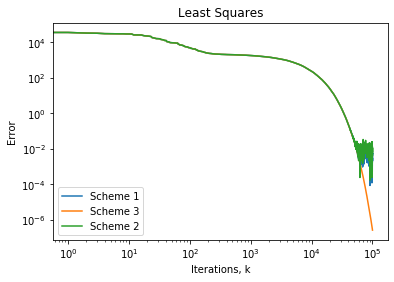
\includegraphics{tex_images/zerothorder_composite_LS}

Rosenbrock: scheme 1,2,3 \newline 

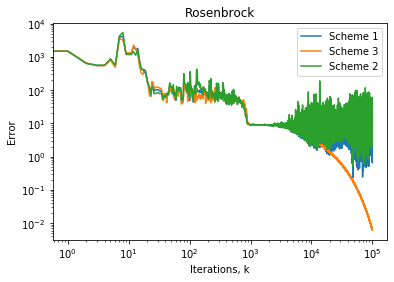
\includegraphics{tex_images/zerothorder_composite_Rosenbrock}

In the Rosenbrock simulations, we set $L_{\nabla f} = \|\nabla^2 f(x_0)\|_2$ where $x_0$ is an initial guess. 



\subsubsection{July 9:}  

By Lemma $3$ in \cite{Nesterov2015}, we claim 

\begin{align}
\|g(x) - \nabla f(x)\|_2 \leq 2\|F(x)\| \frac{\mu}{2}(n+3)^{3/2}\sqrt{\sum_{i=1}^pL_{\nabla F_i}^2}
\end{align}
where $g(x) := 2F(x)\nabla F_{\mu}(x)$. 
\begin{proof}
Let the correlation operator $B^{-1} = I$. Using lemma $3$ on the components of $F$,
\begin{align}
\|g(x) - \nabla f(x)\|^2 & = \| 2F(x)\nabla F(x) - 2F(x)\nabla F_{\mu}(x)\|^2 \notag \\ & \leq  4 \|F(x)\|^2 \| \nabla F(x) - \nabla F_{\mu}(x)\|^2 \notag \\ & \leq  4\|F(x)\|^2 \sum_{i=1}^p \|\nabla F_i(x) - \nabla F_{i,\mu}(x)\|^2  \notag \\ & \leq 4\|F(x)\|^2 \sum_{i=1}^p \frac{\mu^2}{4}L_{\nabla F_i}^2 (n+3)^3 \notag \\ & = 4 \|F(x) \|^2 \frac{\mu^2}{4}(n+3)^3 \sum_{i=1}^p L_{\nabla F_i}^2
\end{align}
\end{proof}

Assuming the components of $F$ are $C^1$ with gradient lipschitz, we have 

\begin{align}
\|F(x) - F_{\mu}(x)\| \leq \frac{\mu^2n}{2}\sqrt{\sum_{i=1}^p L_{\nabla F_i}^2}
\end{align}

\begin{proof}

Using $F_i \in C^1$ with gradient lipschitz and by Theorem $1$ in \cite{Nesterov2015}
\begin{align*}
\|F(x) - F_{\mu}(x)\|^2 & = \sum_{i=1}^p\|F_i(x) - F_{\mu,i}(x)\|^2 \\ & \leq \sum_{i=1}^p\left(\frac{\mu^2}{2}L_{\nabla F_i}n\right)^2 \\ & = \left(\frac{\mu^2}{2}n\right)^2 \sum_{i=1}^p L_{\nabla F_i}^2 
\end{align*}
\end{proof}

Recall equation \eqref{error_bound_approach_3}, the above two facts, and the components of $F$ are lipschitz together yield

\begin{align}
\| \nabla f(x) - \nabla (h \circ F_{\mu})(x)\| & \leq 2\|F(x)\| \underbrace{\|\nabla F(x) - \nabla F_{\mu}(x)\|}_{\text{Use Lemma } 3} + \|\nabla F_{\mu}(x)\| \underbrace{\|F(x) - F_{\mu}(x)\|}_{\text{Use Theorem } 1} \notag \\ & \leq 2\|F(x)\| \frac{\mu}{2}(n+3)^{3/2}\sqrt{\sum_{i=1}^p L_{\nabla F_i}^2} + \sqrt{\sum_{i=1}^pL_{\nabla F_i}^2} \frac{\mu^2n}{2}\sqrt{\sum_{i=1}^pL_{\nabla F_i}^2} \notag \\ & = \sqrt{\sum_{i=1}^pL_{\nabla F_i}^2}\left(2\|F(x)\|\frac{\mu}{2}(n+3)^{3/2} + \frac{\mu^2n}{2}\sqrt{\sum_{i=1}^pL_{\nabla F_i}^2}\right)
\end{align}

Suppose $L_{\nabla F_i} = L_{\nabla F_j}$ for all $i,j$. Then 
\begin{align}
\| \nabla f(x) - \nabla (h \circ F_{\mu})(x)\|  & \leq \sqrt{p}L_{\nabla F_1}\left(2\|F(x)\|\frac{\mu}{2}(n+3)^{3/2} + \frac{\mu^2n\sqrt{p}}{2}L_{\nabla F_1}\right)
\end{align}

\textcolor{red}{Remark:} At the moment, we haven't used any convexity assumptions. \newline 

\textcolor{red}{Derivations of the scheme:} Scheme $1$ in \ref{scheme_composite_struct} is taken from equation $(54)$ in \cite{Nesterov2015}. To justify scheme $2$, observe the following computation:

\begin{align}
\nabla (h \circ F_{\mu}) & = \nabla h(F_{\mu}(x)) \nabla F_{\mu}(x) \notag \\ & = 2F_{\mu}(x)\nabla F_{\mu}(x) \notag \\ & = 2\mathbb{E}_u[F(x+\mu u)] \mathbb{E}_u[\vec{g}_{\mu}(x)] \label{h_compose_F_mu_grad}
\end{align}

where 

\begin{align}
\vec{g}_{\mu}(x) = \begin{bmatrix}
\frac{F_1(x+\mu u) - F_1(x)}{\mu} \\ \vdots \\ \frac{F_p(x+\mu u) - F_p(x)}{\mu}
\end{bmatrix}Bu
\end{align}

$[\vec{g}_{\mu}(x)]_i = g_{i,\mu}(x)$ with $\mathbb{E}_u[g_{i,\mu}(x)] = \nabla F_{i,\mu}(x)$. In view of \eqref{h_compose_F_mu_grad}, we have Scheme $2$ as a result. \newline 

\subsection{July 10}
Scheme $3$ from \ref{scheme_composite_struct} is constructed from Scheme $2$ while ignoring any stochasticity from $F$.
\newpage
Scheme 3:

\begin{align}
x_{k+1} & = x_k - h_k 2F(x_k)\frac{F(x_k+\mu_k u) - F(x_k)}{\mu_k}u
\end{align}

\begin{equation}
g_{3} = 2F(x_k)\frac{F(x_k+\mu_k u) - F(x_k)}{\mu_k}u 
\end{equation}

\begin{equation}
E_{u}[g_{3}] = 2 F(x_k)E_{u}[\vec{g}_{\mu}(x)] 
\end{equation}

\begin{align}
\| \nabla f(x) - E_{u}[g_{3}])\| & \leq 2\|F(x)\| \underbrace{\|\nabla F(x) - \nabla F_{\mu}(x)\|}_{\text{Use Lemma } 3} \notag \\ & \leq 2\|F(x)\| \frac{\mu}{2}(n+3)^{3/2}\sqrt{\sum_{i=1}^p L_{\nabla F_i}^2}
\end{align}

\begin{align}
E_{u}[\|g_{3} - \nabla f(x)\|] &\leq E_{u}[\|g_{3} - E_{u}[g_{3}\|] + \|\nabla f(x) - E_{u}[g_{3}]\|\\
&\leq 2\|F(x_k)\|\left(E_{u}[\|\vec{g}_{\mu}(x )- E_{u}[\vec{g}_{\mu}(x)]\| ] + \frac{\mu}{2}(n+3)^{3/2}\sqrt{\sum_{i=1}^p L_{\nabla F_i}^2} \right)
\end{align}

\section{Week 5: July 13}


\subsection{July 13}

We consider another test problem (Ridge Regression):
\begin{align}
f(x) = \| Ax - b\|^2 + \lambda \|x\|^2
\end{align}
where $\lambda > 0$. Observe on average, $\min_xf(x) > 0$. The first and second derivatives:
\begin{align}
\nabla f(x) & = 2(Ax-b)^\top A + 2\lambda x  \label{ridge_solution}\\ \nabla^2f(x) & = 2(A^\top A + \lambda I)
\end{align}

In view of \eqref{ridge_solution}, the argmin of the ridge regression problem is $x^{\star} = (A^\top A + \lambda I)^{-1}A^\top b$. \newline 

We write $f = h \circ F$ where 
\begin{align}
F(x) = (F_1(x), \dots, F_p(x), G_1(x), \dots, G_n(x))
\end{align}
with
\begin{align}
F_i(x) & = a_i^\top x - b_i \quad \text{ for } 1 \leq i \leq p \\
G_j(x) & = \lambda^{1/2}x_j \quad \text{ for } 1 \leq j \leq n
\end{align}

Here's the simulation for the three schemes (see \ref{scheme_composite_struct}):

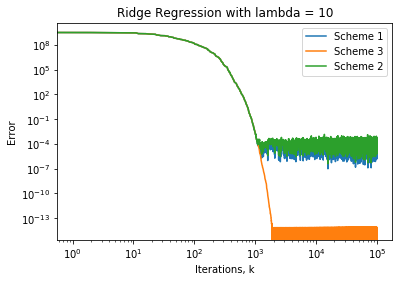
\includegraphics{tex_images/zerothorder_composite_Ridge}

Recall $g_{\mu}(x)= \frac{f(x+\mu u) - f(x)}{\mu}u$ and $g_{\mu,3}(x):= 2F(x)\frac{F(x+\mu u)-F(x)}{\mu}u$. By the triangle inequality and taking expectation,
\begin{align}
\mathbb{E}_u[\| g_{\mu}(x) - \nabla f(x)\|] & \leq \mathbb{E}_u[\|g_{\mu}(x) - \nabla f_{\mu}(x)\|] + \| \nabla f(x) - \nabla f_u(x)\| \notag \\ & \leq \mathbb{E}_u\| g_{\mu}(x) - \nabla f_{\mu}(x)\|] + \frac{\mu}{2}L_{\nabla f}(n+3)^{3/2}
\end{align}
assuming $f \in C^1(E)$ and $f$ has gradient Lipschitz. \newline 

Next, we prove the following.

\begin{theorem} \label{July_13_Theorem_grad_upper_bound}
\begin{align}
\|\nabla F_{\mu}(x) - \nabla F(x) \| \leq \frac{\mu}{2}(n+3)^{3/2}\sqrt{\sum_{i=1}^p L_{\nabla F_i}^2}
\end{align}
\begin{proof}
Assuming the components of $F$ is $C^1$ and has gradient Lipschitz and by Lemma $3$ in \cite{Nesterov2015},
\begin{align}
\|\nabla F_{\mu}(x) - \nabla F(x)\|_2^2 & \leq \|\nabla F_{\mu}(x) - \nabla F(x)\|_F^2 \notag \\ & = \sum_{i=1}^p \| \nabla F_{i,\mu}(x) - \nabla F_i(x)\|_2^2 \notag \\ & \leq \sum_{i=1}^p\left(\frac{\mu}{2}L_{\nabla F_i}(n+3)^{3/2}\right)^2 \notag \\ & = \left(\frac{\mu}{2}(n+3)^{3/2}\right)^2\sum_{i=1}^pL_{\nabla F_i}^2
\end{align}
\end{proof}
\end{theorem}

Using this fact and assuming that $L_{\nabla F_i} = L_{\nabla F_j}$ for all $i,j$,

\begin{align}
\mathbb{E}_u[\| g_{\mu,3}(x) - \nabla f(x)\|] & = \mathbb{E}_u\left[\|2F(x)\left\{\frac{F(x+\mu u) - F(x)}{\mu}u - \nabla F(x)\right\}\|\right] \notag \\ & \leq 2\|F(x)\| \mathbb{E}_u\left[\| \frac{F(x+\mu u) - F(x)}{\mu}u - \nabla F(x)\|\right] \notag \\ & \leq 2\| F(x)\|\mathbb{E}_u\left[\| \frac{F(x+\mu u) - F(x)}{\mu}u - \nabla F_{\mu}(x) \|\right] + 2\|F(x)\| \|\nabla F_{\mu}(x) - \nabla F(x)\| \notag \\ & \leq  2\| F(x)\|\mathbb{E}_u\left[\| \frac{F(x+\mu u) - F(x)}{\mu}u - \nabla F_{\mu}(x) \|\right] + 2\|F(x)\| \frac{\mu}{2}(n+3)^{3/2}\sqrt{p}L_{\nabla F_1} \label{sampling_error_2F_diff_quotient}
\end{align}

Question: How does one deal with $\mathbb{E}_u\|g_{\mu}(x) - \nabla f_{\mu}(x)\|$? If such an approach exists, then dealing $\mathbb{E}_u\left[\| \frac{F(x+\mu u)-F(x)}{\mu}u - \nabla F_{\mu}(x) \|\right]$ can be dealt with similarly. 

\subsection{July 14}

We prove

\begin{theorem} \label{July_14_Big_Theorem_1}


\begin{align}
\mathbb{E}_u[\| g_{\mu}(x) - \nabla f(x)\|] & \leq \mu L_{\nabla f}(n+6)^{3/2} + 2(\sqrt{n} + 3)\|\nabla f(x)\| \label{sampling_error_diff_quotient}
\end{align}
assuming that $f \in C^1(E)$ with lipschitz gradient and is convex. 
\begin{proof}
By Theorem $4$ in \cite{Nesterov2015} and Jensen's inequality, we arrive at 

\begin{align}
\mathbb{E}_u[\|g_{\mu}(x) - \nabla f(x)\|] & \leq \sqrt{\mathbb{E}_u\|g_{\mu}(x) - \nabla f(x)\|^2} \notag \\ & \leq \sqrt{2\mathbb{E}_u\{\|g_{\mu}(x)\|^2 + \|\nabla f(x)\|^2\}} \notag \\ & = \sqrt{2}\sqrt{\mathbb{E}_u\|g_{\mu}(x)\|^2 + \|\nabla f(x)\|^2}  \notag \\ & \leq \sqrt{2}\left(\sqrt{\mathbb{E}_u\|g_{\mu}\|^2} + \|\nabla f(x)\|\right) \notag \\ & \leq \sqrt{2}\left( \sqrt{\frac{\mu^2}{2}L_{\nabla f}^2(n+6)^3 + 2(n+4)\|\nabla f(x)\|^2} + \|\nabla f(x)\|\right) \notag \\ & \leq \sqrt{2}\left( \sqrt{\frac{\mu^2}{2}L_{\nabla f}^2(n+6)^3} + \sqrt{2(n+4)\|\nabla f(x)\|^2} + \|\nabla f(x)\| \right) \notag \\ & = \sqrt{2}\left(\frac{\mu}{\sqrt{2}}L_{\nabla f}(n+6)^{3/2} + \sqrt{2}\sqrt{n+4}\|\nabla f(x)\| + \| \nabla f(x)\|\right) \notag \\ & \leq \mu L_{\nabla f}(n+6)^{3/2} + 2(\sqrt{n} + 3)\|\nabla f(x)\|
\end{align}
\end{proof}

\end{theorem}

By Theorem $2$ and recycling the proof, we have 

\begin{theorem}
\begin{align}
\mathbb{E}_u[\| \hat{g}_{\mu}(x) - \nabla f(x)\|] \leq \frac{\mu}{2}L_{\nabla f}(n+6)^{3/2} + 2(\sqrt{n}+3)\|\nabla f(x)\| \label{central_diff_sampling_error}
\end{align}

\end{theorem}

Assume the components of $F$ are $C^1(E)$ with lipschitz gradient and is convex. \newline 

\begin{theorem}

We prove
\begin{align}
\mathbb{E}_u[\| g_{\mu,3}(x) - \nabla f(x)\|] & \leq 2\|F(x)\|\left\{\sum_{i=1}^p \mu L_{\nabla F_i}(n+6)^{3/2} + 2(\sqrt{n} + 3)\|\nabla F_i(x)\|\right\}
\end{align}
\begin{proof}
Using \eqref{sampling_error_2F_diff_quotient} and recycling the proof of the fact \eqref{sampling_error_diff_quotient}, we have 
\begin{align}
\mathbb{E}_u\| \frac{F(x+\mu u) - F(x)}{\mu}u - \nabla F(x) \|_2 & \leq \mathbb{E}_u\| \frac{F(x+\mu u) - F(x)}{\mu}u - \nabla F(x)\|_F \notag \\ & = \mathbb{E}_u\sqrt{\sum_{i=1}^p\| \frac{F_i(x+\mu u) - F_i(x)}{\mu}u - \nabla F_i(x) \|^2} \notag \\ & \leq \mathbb{E}_u \sum_{i=1}^p \| \frac{F_i(x+\mu u) - F_i(x)}{\mu}u - \nabla F_i(x)\| \notag \\ & = \sum_{i=1}^p \mathbb{E}_u\| \frac{F_i(x+\mu u) - F_i(x)}{\mu}u - \nabla F_i(x)\| \notag \\ & \leq \sum_{i=1}^p\left\{\mu L_{\nabla F_i}(n+6)^{3/2} + 2(\sqrt{n} + 3)\|\nabla F_i(x)\| \right\}
\end{align}
Therefore, the conclusion follows. Observe if we assume $L_{\nabla F_i} = L_{\nabla F_j}$ for all $i,j$, 
\begin{align}
\mathbb{E}_u\|g_{\mu,3}(x) - \nabla f(x)\| & \leq 2\|F(x)\|\left\{p\mu L_{\nabla F_1}(n+6)^{3/2} + 2p(\sqrt{n}+3)\max_{1 \leq i \leq p}\|\nabla F_i(x)\| \right\}
\end{align}
\end{proof}

\end{theorem}

Then using \eqref{central_diff_sampling_error}, we have


\begin{theorem}

\begin{align}
\mathbb{E}_u\left[\left\| \frac{F(x+\mu u) - F(x-\mu u)}{2\mu}u - \nabla F(x)\right\|\right] & \leq \sum_{i=1}^p\left\{\frac{\mu}{2}L_{\nabla F_i}(n+6)^{3/2} + 2(\sqrt{n} + 3)\|\nabla F_i(x)\|\right\}
\end{align}
Consequently, 
\begin{align}
\mathbb{E}_u[\| \hat{g}_{\mu,3}(x) - \nabla f(x) \|] \leq 2\|F(x)\|\sum_{i=1}^p\left\{\frac{\mu}{2}L_{\nabla F_i}(n+6)^{3/2} + 2(\sqrt{n} + 3)\|\nabla F_i(x)\|\right\}
\end{align}
Assume that $L_{\nabla F_i} = L_{\nabla F_j}$ for all $i,j$, we have 
\begin{align}
\mathbb{E}_u\left[\left\| \frac{F(x+\mu u) - F(x-\mu u)}{2\mu}u - \nabla F(x)\right\|\right] & \leq \frac{\mu}{2}pL_{\nabla F_1}(n+6)^{3/2} + 2p(\sqrt{n} + 3)\max_{1 \leq i \leq p}\|\nabla F_i(x)\| 
\end{align}
Consequently,
\begin{align}
\mathbb{E}_u[\| \hat{g}_{\mu,3}(x) - \nabla f(x) \|] & \leq 2\|F(x)\|\left[\frac{\mu}{2}pL_{\nabla F_1}(n+6)^{3/2} + 2p(\sqrt{n} + 3)\max_{1 \leq i \leq p}\|\nabla F_i(x)\| \right]
\end{align}

\end{theorem}

\subsection{July 15}

\begin{lemma} \label{July_15_Lemma}
\begin{align*}
\mathbb{E}_u\left[\left\| \frac{F(x+\mu u) - F(x)}{\mu}u - \nabla F(x) \right\|^2\right] & \leq \sum_{i=1}^p\left(\mu^2L_{\nabla F_i}^2(n+6)^3 + 4(n+5)\|\nabla F_i(x)\|^2\right)
\end{align*}
\begin{proof}
\begin{align*}
\mathbb{E}_u\left[\left\| \frac{F(x+\mu u)-F(x)}{\mu}u - \nabla F(x) \right\|^2\right] & \leq \mathbb{E}_u\left[\left\|\frac{F(x+\mu u)-F(x)}{\mu}u - \nabla F(x)\right\|_F^2\right] \\ & = \sum_{i=1}^p\mathbb{E}_u\left[\left\|\frac{F_i(x+\mu u)-F_i(x)}{\mu}u - \nabla F_i(x)  \right\|^2\right] \\ & \leq 2\sum_{i=1}^p\left( \mathbb{E}_u\left[\left\| \frac{F_i(x+\mu u) - F_i(x)}{\mu}u \right\|^2 \right] + \|\nabla F_i(x)\|^2\right) \\ & \leq 2\sum_{i=1}^p\left(\frac{\mu^2}{2}L_{\nabla F_i}^2(n+6)^3 + 2(n+4)\|\nabla F_i(x)\|^2 + \| \nabla F_i(x)\|^2\right) \\ & \leq 2\sum_{i=1}^p\left(\frac{\mu^2}{2}L_{\nabla F_i}^2(n+6)^3 + 2(n+5)\|\nabla F_i(x)\|^2\right)
\end{align*}
\end{proof}
\end{lemma}

\begin{lemma}
\begin{align*}
\mathbb{E}_u\left[\left\|\frac{F(x+\mu u)-F(x-\mu u)}{2\mu}u - \nabla F(x)\right\|^2\right] & \leq \sum_{i=1}^p\left(\frac{\mu^2}{4}L_{\nabla F_i}^2(n+6)^3 + 4(n+5)\|\nabla F_i(x)\|^2\right)
\end{align*}

\begin{proof}
\begin{align*}
\mathbb{E}_u\left[\left\| \frac{F(x+\mu u)-F(x-\mu u)}{2\mu}u - \nabla F(x) \right\|^2 \right] & \leq \mathbb{E}_u\left[\left\| \frac{F(x+\mu u)-F(x-\mu u)}{2\mu}u - \nabla F(x) \right\|_F^2\right] \\ & = \sum_{i=1}^p \mathbb{E}_u\left[\left\| \frac{F_i(x+\mu u) - F_i(x-\mu u)}{2\mu }u - \nabla F_i(x) \right\|^2\right] \\ & \leq 2\sum_{i=1}^p\left(\mathbb{E}_u\left[\left\|\frac{F_i(x+\mu u) - F_i(x-\mu u)}{2\mu}u\right\|^2\right] + \| \nabla F_i(x)\|^2\right) \\ & \leq 2\sum_{i=1}^p\left(\frac{\mu^2}{8}L_{\nabla F_i}^2 (n+6)^3 + 2(n+4)\|\nabla F_i(x)\|^2 + \|\nabla F_i(x)\|^2\right) \\ & \leq 2\sum_{i=1}^p\left(\frac{\mu^2}{8}L_{\nabla F_i}^2(n+6)^3 + 2(n+5)\|\nabla F_i(x)\|^2\right) \\ & = \sum_{i=1}^p\left(\frac{\mu^2}{4}L_{\nabla F_i}^2(n+6)^3 + 4(n+5)\|\nabla F_i(x)\|^2\right)
\end{align*}
\end{proof}
\end{lemma}

Define $g_{\mu,2}(x) = 2F(x+\mu u)\left[\frac{F(x+\mu u)-F(x)}{\mu}\right]u$. \newline 

We have the following fact:

\begin{theorem}


\begin{align}
\mathbb{E}_u\left\| g_{\mu,2}(x) - \nabla f(x) \right\| & \leq 2L_F\mu\left[n + \sum_{i=1}^p\left\{\mu^2L_{\nabla F_i}^2(n+6)^3 + 4(n+5)\|\nabla F_i(x)\|^2\right\}\right] \notag \\ & + 2\|F(x)\|\sum_{i=1}^p\left\{\mu L_{\nabla F_i}(n+6)^{3/2} + 2(\sqrt{n} + 3)\|\nabla F_i(x)\|\right\} + 2L_F^2\mu\sqrt{n}
\end{align}

Assuming $L_{\nabla F_i} = L_{\nabla F_j}$ for all $i,j$, we have 
\begin{align}
\mathbb{E}_u\left\| g_{\mu,2}(x) - \nabla f(x) \right\| & \leq 2L_F\mu\left[n + p\mu^2L_{\nabla F_1}^2(n+6)^3 + 4(n+5)\|\nabla F(x)\|_F^2\right] \notag \\ & + 2\|F(x)\|\left\{p\mu L_{\nabla F_1}(n+6)^{3/2} + 2p(\sqrt{n}+3)\max_{1 \leq i \leq p}\|\nabla F_i(x)\|\right\} + 2L_F^2\mu \sqrt{n}
\end{align}

\begin{proof}
\begin{align*}
\left\| g_{\mu,2}(x) - \nabla f(x) \right\| & \leq \left\| 2F(x+\mu u)\left[\frac{F(x+\mu u) - F(x)}{\mu}u - \nabla F(x)\right] \right\|  + \| [2F(x+\mu u) - 2F(x)] \nabla F(x) \| \\ & \leq 2\| F(x+\mu u)\|\left\| \frac{F(x+\mu u) - F(x)}{\mu}u - \nabla F(x) \right\| + 2\|\nabla F(x)\| \|F(x+\mu u) - F(x)\|
\end{align*}
Taking expectation of the above equation and using Jensen's inequality, we have 

\begin{align}
\mathbb{E}_u\left\| g_{\mu,2}(x) - \nabla f(x) \right\| & \leq 2\mathbb{E}_u\left[\| F(x+\
\mu u) - F(x) \| \left\| \frac{F(x+\mu u) - F(x)}{\mu}u - \nabla F(x) \right\|\right] \notag \\ & \leq 2\mathbb{E}_u\left[\|F(x)\| \left\| \frac{F(x+\mu u) - F(x)}{\mu}u - \nabla F(x) \right\|\right]  + 2L_F^2\mu\sqrt{n} \notag \\ & \leq 2L_F \mu \mathbb{E}_u\left[\|u\| \left\| \frac{F(x+\mu u) - F(x)}{\mu}u - \nabla F(x) \right\|\right] \notag \\ & + 2\mathbb{E}_u\left[\|F(x)\| \left\| \frac{F(x+\mu u) - F(x)}{\mu}u - \nabla F(x) \right\|\right] + 2L_F^2\mu \sqrt{n} \notag \\ & \leq 2L_F \mu \mathbb{E}_u\left[\|u\|^2 +  \left\| \frac{F(x+\mu u) - F(x)}{\mu}u - \nabla F(x) \right\|^2\right] \notag \\ & + 2\mathbb{E}_u\left[\|F(x)\| \left\| \frac{F(x+\mu u) - F(x)}{\mu}u - \nabla F(x) \right\|\right] + 2L_F^2\mu \sqrt{n} \notag \\ & \leq 2L_F\mu\left[n + \sum_{i=1}^p(\mu^2L_{\nabla F_i}^2(n+6)^3 + 4(n+5)\|\nabla F_i(x)\|^2)\right] \notag \\ & + 2\|F(x)\| \sum_{i=1}^p\left\{\mu L_{\nabla F_i}(n+6)^{3/2} + 2(\sqrt{n}+3)\|\nabla F_i(x)\|\right\} + 2L_F^2\mu\sqrt{n}
\end{align}

Assuming $L_{\nabla F_1} = L_{\nabla F_j}$ for all $j$, we have 

\begin{align}
\mathbb{E}_u\left\| g_{\mu,2}(x) - \nabla f(x) \right\| & \leq 2L_F\mu\left[n + p\mu^2 L_{\nabla F_1}^2(n+6)^3 + 4(n+5)\|\nabla F(x)\|_F^2\right] \notag \\ & + 2\|F(x)\|\left\{p\mu L_{\nabla F_1}(n+6)^{3/2} + 2p(\sqrt{n}+3)\max_{1 \leq i \leq p}\|\nabla F_i(x)\|\right\} + 2L_F^2\mu \sqrt{n}
\end{align}

\end{proof}

\end{theorem}


We have the following fact:

\begin{theorem}
\begin{align}
\mathbb{E}_u\left\| \hat{g}_{\mu,2}(x) - \nabla f(x) \right\| & \leq 2L_F\mu\left[n + \sum_{i=1}^p\left\{\frac{\mu^2}{4}L_{\nabla F_i}^2(n+6)^3 + 4(n+5)\|\nabla F_i(x)\|^2\right\}\right] \notag \\ & + 2\|F(x)\|\sum_{i=1}^p\left\{\frac{\mu}{2}L_{\nabla F_i}(n+6)^{3/2} + 2(\sqrt{n}+3)\|\nabla F_i(x)\|\right\} + 2L_F^2\mu\sqrt{n} 
\end{align}

Assuming $L_{\nabla F_i} = L_{\nabla F_j}$ for all $i,j$, we have 
\begin{align}
\mathbb{E}_u\left\| \hat{g}_{\mu,2}(x) - \nabla f(x) \right\| & \leq 2L_F\mu\left[n + \frac{p\mu^2}{4}L_{\nabla F_1}^2(n+6)^3 + 4(n+5)\|\nabla F(x)\|_F^2\right] \notag  \\ & + 2\|F(x)\|\left[\frac{p\mu}{2}L_{\nabla F_1}(n+6)^{3/2} + 2p(\sqrt{n} + 3)\max_{1 \leq i \leq p}\|\nabla F_i(x)\|\right] + 2L_F^2\mu\sqrt{n}
\end{align}

\begin{proof}
\begin{align*}
\left\| \hat{g}_{\mu,2}(x) - \nabla f(x) \right\| & \leq \left\|2F(x+\mu u)\left[\frac{F(x+\mu u)-F(x-\mu u)}{2\mu}u - \nabla F(x)\right]\right\| + \|[2F(x+\mu u)-2F(x)]\nabla F(x)\| \\ & \leq 2\|F(x+\mu u)\| \left\| \frac{F(x+\mu u)-F(x-\mu u)}{2\mu}u - \nabla F(x) \right\| + 2\|\nabla F(x)\| \|F(x+\mu u) - F(x)\| \\ & \leq  2[\|F(x+\mu u) - F(x)\|]\left\|\frac{F(x+\mu u) - F(x-\mu u)}{2\mu}u - \nabla F(x)\right\| \\ & + 2[\|F(x)\|]\left\|\frac{F(x+\mu u) - F(x-\mu u)}{2\mu}u - \nabla F(x)\right\| + 2L_F^2\mu \|u\| \\ & \leq 2L_F\mu\|u\|\left\|\frac{F(x+\mu u)-F(x-\mu u)}{2\mu}u - \nabla F(x)\right\| \\ & + 2\|F(x)\|\left\| \frac{F(x+\mu u)-F(x-\mu u)}{2\mu}u - \nabla F(x) \right\| + 2L_F^2\mu \|u\|
\end{align*}

Taking the expectation of both sides,

\begin{align*}
\mathbb{E}_u\left[\left\| \hat{g}_{\mu,2}(x) - \nabla f(x) \right\|\right] & \leq 2L_F\mu\mathbb{E}_u\left[\|u\|\left\| \frac{F(x+\mu u)-F(x-\mu u)}{2\mu}u - \nabla F(x) \right\| \right] \\ & + 2\|F(x)\|\mathbb{E}_u\left[\left\| \frac{F(x+\mu u) - F(x-\mu u)}{2\mu}u - \nabla F(x) \right\|\right] + 2L_F^2\mu \sqrt{n} \\ & \leq  2L_F\mu\mathbb{E}_u\|u\|^2 + 2L_F^2\mu\sqrt{n} + 2L_F\mu\mathbb{E}_u\left[\left\| \frac{F(x+\mu u)-F(x-\mu u)}{2\mu}u - \nabla F(x) \right\|^2 \right] \\ & + 2\|F(x)\|\mathbb{E}_u\left[\left\| \frac{F(x+\mu u)-F(x-\mu u)}{2\mu}u - \nabla F(x) \right\|\right] \\ & \leq 2L_F^2\mu\sqrt{n} + 2L_F\mu n  + 2L_F\mu \sum_{i=1}^p\left\{\frac{\mu^2}{4}L_{\nabla F_i}^2(n+6)^3 + 4(n+5)\|\nabla F_i(x)\|^2\right\} \\ & + 2\|F(x)\|\sum_{i=1}^p\left\{\frac{\mu}{2}L_{\nabla F_i}(n+6)^{3/2} + 2(\sqrt{n} + 3)\|\nabla F_i(x)\|\right\} 
\end{align*}

Assuming $L_{\nabla F_i} = L_{\nabla F_j}$ for all $i,j$, we have 

\begin{align*}
\mathbb{E}_u\left[\left\| \hat{g}_{\mu,2}(x) - \nabla f(x) \right\|\right] & \leq  2L_F\mu[n + \frac{p\mu^2}{4}L_{\nabla F_1}^2(n+6)^3 + 4(n+5)\|\nabla F(x)\|_F^2] \\ & + 2\|F(x)\|\left[\frac{p\mu}{2}L_{\nabla F_1}(n+6)^{3/2} + 2p(\sqrt{n}+3)\max_{1 \leq i \leq p}\|\nabla F_i(x)\|\right] + 2L_F^2\mu \sqrt{n}
\end{align*} 
\end{proof}
\end{theorem}

Recall the following: \newline 
\begin{align}
g_{\mu}(x) & = \frac{f(x+\mu u) - f(x)}{\mu}u \\ \hat{g}_{\mu}(x) & = \frac{f(x+\mu u) - f(x-\mu u)}{2\mu}u \\ g_{\mu,2}(x) & = 2F(x+\mu u)\left[\frac{F(x+\mu u) - F(x)}{\mu}\right]u \\ \hat{g}_{\mu,2}(x) & = 2F(x+\mu u)\left[\frac{F(x+\mu u) - F(x- \mu u)}{2\mu}\right]u \\ g_{\mu,3}(x) & = 2F(x)\left[\frac{F(x+\mu u) - F(x)}{\mu}\right]u \\ \hat{g}_{\mu,3}(x) & = 2F(x)\left[\frac{F(x+\mu u)-F(x-\mu u)}{2\mu}\right]u
\end{align}

Let $g$ be the gradient estimate above. We assume $L_{\nabla F_1} = L_{\nabla F_i}$ for all $1 \leq i \leq p$. \newline 

\label{sampling_error_table}
\begin{center}
\begin{tabular}{l | c  |}
\hline 
\textcolor{red}{error} & $\mathbb{E}_u[\| g - \nabla f(x) \|] \leq $ \textcolor{red}{error} \\ \hline
S1 FD & $\mu L_{\nabla f}(n+6)^{3/2} + 2(\sqrt{n}+3)\|\nabla f(x)\|$ \\ \hline 
 S1 CD & $\frac{\mu}{2}L_{\nabla f}(n+6)^{3/2} + 2(\sqrt{n}+3)\| \nabla f(x)\|$  \\ \hline
S2 FD & \tiny$2L_F\mu[n + p\mu^2 L_{\nabla F_1}^2(n+6)^3 + 4(n+5)\|\nabla F(x)\|_F^2] + 2\|F(x)\|\left\{p\mu L_{\nabla F_1}(n+6)^{3/2} + 2p(\sqrt{n}+3)\max_{1 \leq i \leq p}\|\nabla F_i(x)\|\right\} + 2L_F^2\mu \sqrt{n}$ \\ \hline 
S2 CD & \tiny $2L_F\mu \left[n + \frac{p\mu^2}{4}L_{\nabla F_1}^2 (n+6)^3 + 4(n+5)\|\nabla F(x)\|_F^2\right] + 2\|F(x)\|\left[\frac{p\mu}{2}L_{\nabla F_1}(n+6)^{3/2} + 2p(\sqrt{n}+3)\max_{1 \leq i \leq p}\|\nabla F_i(x)\|\right] + 2L_F^2\mu\sqrt{n}$ \\ \hline 
S3 FD & $2\|F(x)\|\left\{p\mu L_{\nabla F_1}(n+6)^{3/2} + 2p(\sqrt{n}+3)\max_{1 \leq i \leq p}\|\nabla F_i(x)\|\right\}$ \\ \hline
S3 CD & $2\|F(x)\|\left\{\frac{\mu}{2}p L_{\nabla F_1}(n+6)^{3/2} + 2p(\sqrt{n}+3)\max_{1 \leq i \leq p}\|\nabla F_i(x)\|\right\}$ \\ \hline
\hline 
\end{tabular}
\end{center}

\section{Week 6: July 20}

\subsection{July 20} \label{July_20}

For notational brevity, $g_{\mu}(x) = 2F(x)\left[\frac{F(x+\mu u)-F(x)}{\mu}\right]u$. \newline 

We try to mimc the convergence analysis in Theorem $8$ in \cite{Nesterov2015}. \newline 

Compute $\mathbb{E}_u\|g_{\mu}(x)\|^2$.

\begin{align}
g_{\mu}(x) = 2\sum_{i=1}^pF_i(x)g_{\mu,i}(x)u
\end{align}

\begin{align}
\|g_{\mu}(x)\|^2 & \leq 4\|F(x)\|^2\left\| \frac{F(x+\mu u)-F(x)}{\mu}u \right\|^2
\end{align}

\begin{align}
\mathbb{E}_u\|g_{\mu}(x)\|^2 & \leq 4\|F(x)\|^2 \mathbb{E}_u\left[\left\| \frac{F(x+\mu u)-F(x)}{\mu}u \right\|^2\right] \notag \\ & \leq 4\|F(x)\|^2\sum_{i=1}^p\frac{\mu^2}{2}L_{\nabla F_i}^2(n+6)^3 + 2(n+4)\|\nabla F_i(x)\|^2 \notag \\ & = 4\|F(x)\|^2\sum_{i=1}^p\frac{\mu^2}{2}L_{\nabla F_i}^2(n+6)^3 + 2(n+4)\|\nabla F_i(x)\|^2 \label{scheme_3_second_moment}
\end{align}

Define sequence $x_{k+1} = x_k - hg_{\mu}(x_k)$ and $r_k = \|x_k-x^*\|$ where $x^*$ is the optimal solution to minimizing $f(x)$. \newline 

\begin{align}
r_{k+1}^2 & = \|x_{k+1} - x^*\|^2\notag  \\ & = \|x_k - hg_{\mu}(x_k) - x^*\|^2 \notag \\ & = \|x_k - x^* - hg_{\mu}(x_k)\|^2 \notag \\ & = r_k^2 - 2h\langle g_{\mu}(x_k),x_k-x^*\rangle + h^2\| g_{\mu}(x_k)\|^2
\end{align}

Observe that
\begin{align}
\mathbb{E}_ug_{\mu}(x_k) & = 2\sum_{i=1}^pF_i(x_k)\nabla F_{\mu,i}(x_k)
\end{align}

\begin{align}
\mathbb{E}_{u_k}(r_{k+1}^2) & \leq r_k^2 - 2h\left\langle \sum_{i=1}^p 2F_i(x_k)\nabla F_{\mu,i}(x_k), x_k - x^*\right\rangle + 2\|F(x_k)\|^2h^2\sum_{i=1}^p\frac{\mu^2}{2}L_{\nabla F_i}^2(n+6)^3 + 2(n+4)\|\nabla F_i(x_k)\|^2 \notag \\ & = r_k^2 - 2h\sum_{i=1}^p\left\langle 2F_i(x_k)\nabla F_{\mu,i}(x_k), x_k - x^*\right\rangle + 2\|F(x_k)\|^2h^2\sum_{i=1}^p\frac{\mu^2}{2}L_{\nabla F_i}^2(n+6)^3 + 2(n+4)\|\nabla F_i(x_k)\|^2 \notag  \\ & = r_k^2 - 2h\sum_{i=1}^p2F_i(x_k)\langle \nabla F_{\mu,i}(x_k), x_k - x^*\rangle + 2\|F(x_k)\|^2h^2\sum_{i=1}^p\frac{\mu^2}{2}L_{\nabla F_i}^2(n+6)^3 + 2(n+4)\|\nabla F_i(x_k)\|^2 \notag \\ & \leq r_k^2 - 2h\sum_{i=1}^p2F_i(x_k)\left[F_i(x_k) - F_{i,\mu}(x^*)\right] + 2\|F(x_k)\|^2h^2\sum_{i=1}^p\frac{\mu^2}{2}L_{\nabla F_i}^2(n+6)^3 + 4(n+4)L_{\nabla F_i}(F_i(x_k) - F_i(x^*))
\end{align}

\begin{lemma} \label{Lipschitz_grad_f}
Assume $F_i, \nabla F_i$ are Lipschitz continuous for all $1 \leq i \leq p$. Then 
\begin{align}
\|\nabla f(x) - \nabla f(y)\| \leq L_{\nabla f}(x,y)\|x-y\| \quad \forall x,y \in \mathbb{R}^n
\end{align}


where $L_{\nabla f}(x,y) = L_{\nabla F}^2 + 2L_F^2 + \|F(x)\|^2$ with 
\begin{align}
L_F & = \sqrt{\sum_{i=1}^pL_{F_i}^2} \\ L_{\nabla F} & = \sqrt{\sum_{i=1}^pL_{\nabla F_i}^2}
\end{align}

\begin{proof}
Recall

\begin{align}
\nabla f(x) - \nabla f(y) = 2\sum_{i=1}^p\left\{ F_i(x)[\nabla F_i(x)-\nabla F_i(y)] + [F_i(x)-F_i(y)]\nabla F_i(y) \right\} 
\end{align}

By hypothesis,

\begin{align*}
\| \nabla f(x) - \nabla f(y)\| & = 2\left\| \sum_{i=1}^pF_i(x)[\nabla F_i(x)-\nabla F_i(y)] + [F_i(x) - F_i(y)]\nabla F_i(y) \right\| \\ & \leq 2\sum_{i=1}^p\| F_i(x)\| \|\nabla F_i(x) - \nabla F_i(y)\| + \|F_i(x)-F_i(y)\| \|\nabla F_i(y)\| \\ & \leq 2\sum_{i=1}^p\| F_i(x)\| L_{\nabla F_i}\|x-y\| + L_{F_i}^2\|x-y\| \\ & = \sum_{i=1}^p\left(2L_{\nabla F_i}\|F_i(x)\| + 2L_{F_i}^2\right)\|x-y\| \\ & = \|x-y\| \sum_{i=1}^p\left(2L_{\nabla F_i}\|F_i(x)\| + 2L_{F_i}^2\right) \\ & = \|x-y\|\left(\sum_{i=1}^p2L_{\nabla F_i}\|F_i(x)\| + \sum_{i=1}^p2L_{F_i}^2\right) \\ & \leq \|x-y\|\left(\sum_{i=1}^pL_{\nabla F_i}^2 + \|F_i(x)\|^2 + 2\sum_{i=1}^pL_{F_i}^2\right) \\ & \leq \|x-y\|\left(L_{\nabla F}^2 + \|F(x)\|^2 + 2L_F^2\right) \\ & = \|x-y\|L_{\nabla f}(x,y)
\end{align*}

\end{proof}
\end{lemma}

Unless stated otherwise, assume $g_{\mu}(x) = 2F(x)\left[\frac{F(x+\mu u)-F(x)}{\mu}\right]u$. In our setting, 

\begin{align} f(x) & = \|F(x)\|^2, \\ x_{k+1} & = x_k - hg_{\mu}(x_k). \end{align} 

Second approach to convergence analysis: \newline 

\begin{align*}
f(x_{k+1}) & \leq f(x_k) + \langle \nabla f(x_k), -hg_{\mu}(x_k)\rangle + \frac{L_{\nabla f}}{2}\|hg_{\mu}(x_k)\|^2 \\ & = f(x_k) -h \langle \nabla f(x_k),g_{\mu}(x_k)\rangle + \frac{L_{\nabla f}}{2}h^2\|g_{\mu}(x_k)\|^2
\end{align*}

By \eqref{scheme_3_second_moment}, 

\begin{align*}
\mathbb{E}_{u_k}f(x_{k+1}) & \leq f(x_k) - h\mathbb{E}_{u_k}\langle \nabla f(x_k), g_{\mu}(x_k)\rangle + \frac{L_{\nabla f}}{2}h^2\mathbb{E}_{u_k}\|g_{\mu}(x_k)\|^2 \\ & \leq f(x_k) - h\mathbb{E}_{u_k}\langle \nabla f(x_k), g_{\mu}(x_k)\rangle + \frac{L_{\nabla f}}{2}h^2\left[2\|F(x_k)\|^2\sum_{i=1}^p\frac{\mu^2}{2}L_{\nabla F_i}^2(n+6)^3 + 2(n+4)\| \nabla F_i(x_k)\|^2 \right]
\end{align*}

%\textcolor{red}{Question}: $L_{\nabla f}(x,y):= L_{\nabla F}^2 + \|F(x)\|^2 + 2L_F^2$ in Lemma \ref{Lipschitz_grad_f} and replacing this in the table \ref{sampling_error_table} doesn't exactly work. The results from this table utilize Theorem $4$ in \cite{Nesterov2015}, which makes use of the constant $L_{\nabla f}$. Replacing $L_{\nabla f}$ in this thoerem with $L_F^2 + \|F(x)\|^2 + 2L_F^2$ doesn't exactly work without modification. Is this worth pursuing? To circumvent this, I can assume that $F_i$'s are bounded for all $1 \leq i \leq p$ in the proof of Lemma \ref{Lipschitz_grad_f}, but should we make such assumption?

\subsection{July 21}

\begin{lemma} \label{July_21_quadratic_upperbound}
Assume $F_i, \nabla F_i$ are Lipschitz continuous for all $1 \leq i \leq p$. Then for all $x,y \in \mathbb{R}^n$,
\begin{align}
|f(x) - f(y) - \nabla f(y)(x-y)| \leq \frac{1}{2}(L_{\nabla F}^2 + 2L_F^2 + \|F(y)\|^2)\|x-y\|^2
\end{align}

\begin{proof}
By the following computation and lemma \ref{Lipschitz_grad_f},

\begin{align*}
|f(x) - f(y) - \nabla f(y)(x-y)| & = \left|\int_0^1[\nabla f(y+t(x-y)) - \nabla f(y)](x-y)dt\right| \\ & \leq \int_0^1\| \nabla f(y+t(x-y)) - \nabla f(y) \| \|x-y\| dt \\ & = \int_0^1(L_{\nabla F}^2 + 2L_F^2 + \|F(y)\|^2)\|x-y\|^2tdt \\ & = \frac{1}{2}(L_{\nabla F}^2 + 2L_F^2 + \|F(y)\|^2)\|x-y\|^2
\end{align*}
\end{proof}
\end{lemma}

\begin{theorem} \label{Theorem_July_21_second_moment}
Remark: We prove a result analogous to theorem $4$ in \cite{Nesterov2015}, which we state here. Recall that $g_{\mu}(x) = \frac{f(x+\mu u)-f(x)}{\mu}u$ and $\hat{g}_{\mu}(x) = \frac{f(x+\mu u)-f(x-\mu u)}{2\mu}u$. Then

\begin{align}
\mathbb{E}_u(\|g_{\mu}(x)\|^2) & \leq \frac{1}{2}(L_{\nabla F}^2 + 2L_F^2 + \|F(x)\|^2)^2\mu^2(n+6)^3 + 2(n+4)\|\nabla f(x)\|^2 \\ \mathbb{E}_u(\|\hat{g}_{\mu}(x)\|^2) & \leq \frac{\mu^2}{8}(L_{\nabla F}^2 + 2L_F^2 + \|F(x)\|^2)^2(n+6)^3 + 2(n+4)\|\nabla f(x)\|^2
\end{align}

\begin{proof}
By Young's inequality and lemma \ref{July_21_quadratic_upperbound}, we have 

\begin{align*}
[f(x+\mu u) - f(x)]^2 & = [f(x+\mu u) - f(x) - \langle \nabla f(x), \mu u\rangle + \langle \nabla f(x), \mu u\rangle ]^2 \\ & \leq 2(f(x+\mu u) - f(x) - \langle \nabla f(x), \mu u\rangle)^2 + 2\mu^2\langle \nabla f(x),\mu\rangle^2  \\ & \leq 2\left(\frac{1}{2}(L_{\nabla F}^2 + 2L_F^2 + \|F(x)\|^2)\mu^2 \|u\|^2\right)^2 + 2\mu^2 \langle \nabla f(x),u\rangle^2 \\ & = \frac{1}{2}(L_{\nabla F}^2 + 2L_F^2 + \|F(x)\|^2)^2\mu^4 \|u\|^4 + 2\mu^2 \langle \nabla f(x),u\rangle^2
\end{align*}

Dividing both sides by $\mu^2$, taking expectation, multiplying by $\|u\|^2$, and following the steps in Nesterov's proof $4.2$ equation $(35)$, we have 

\begin{align*}
\mathbb{E}_u(\|g_{\mu}(x)\|^2) & \leq \frac{1}{2}(L_{\nabla F}^2 + 2L_F^2 + \|F(x)\|^2)^2\mu^2\mathbb{E}_u(\|u\|^6) + 2\mathbb{E}_u[\langle  \nabla f(x),u \rangle^2\|u\|^2] \\ & \leq \frac{1}{2}(L_{\nabla F}^2 + 2L_F^2 + \|F(x)\|^2)^2 \mu^2 (n+6)^3 + 2(n+4)\|\nabla f(x)\|^2
\end{align*}

For the symmetric oracle $\hat{g}_{\mu}$, since $f$ is convex, we have 

\begin{align*}
f(x+\mu u) - f(x-\mu u) & = [f(x+\mu u) - f(x)] + [f(x) - f(x-\mu u)] \\ & \leq [\langle \nabla f(x),\mu u\rangle + \frac{\mu^2}{2}(L_{\nabla F}^2 + 2L_F^2 + \|F(x)\|^2)\|u\|^2] + \mu \langle \nabla f(x),u\rangle  \\ & = 2\mu\langle \nabla f(x),u\rangle + \frac{\mu^2}{2}(L_{\nabla F}^2 + 2L_F^2 + \|F(x)\|^2)\|u\|^2
\end{align*}

Similarly, we claim that $f(x+\mu u) - f(x-\mu u) \geq 2\mu\langle \nabla f(x),u\rangle - \frac{\mu^2}{2}(L_{\nabla F}^2 + 2L_F^2 + \|F(x)\|^2)\|u\|^2$. To see this, we have 

\begin{align*}
f(x+ \mu u) - f(x) \geq \langle \nabla f(x), \mu u\rangle
\end{align*}
by convexity. So it suffices to deduce 

\begin{align}
f(x)-f(x-\mu u) \geq \langle \nabla f(x),\mu u\rangle - \frac{\mu^2}{2}(L_{\nabla F}^2 + 2L_F^2 + \|F(x)\|^2)\|u\|^2 \label{July_21_lower_bound_quadratic}
\end{align}

By lemma \ref{July_21_quadratic_upperbound}, we have 

\begin{align*}
|f(x-\mu u) - f(x) - \langle \nabla f(x), -\mu u \rangle | & \leq \frac{\mu^2}{2}(L_{\nabla F}^2 + 2L_F^2 + \|F(x)\|^2)\|u\|^2
\end{align*}

This implies 

\begin{align*}
f(x) - f(x-\mu u) - \langle \nabla f(x),\mu u\rangle  & \geq -\frac{\mu^2}{2}(L_{\nabla F}^2 + 2L_F^2 + \|F(x)\|^2)\|u\|^2
\end{align*}

This implies \eqref{July_21_lower_bound_quadratic}. Therefore, by Young's inequality and following Nesterov's proof for theorem $4.2$ in \cite{Nesterov2015}, we have

\begin{align*}
\mathbb{E}_u(\| \hat{g}_{\mu}(x) \|^2) & =  \frac{1}{4\mu^2}\mathbb{E}_u([ f(x+\mu u) - f(x-\mu u) - 2\mu\langle \nabla f(x),u\rangle + 2\mu \langle \nabla f(x),u\rangle ]^2\|u\|^2) \\ & \leq \frac{1}{2\mu^2}\mathbb{E}_u([f(x+\mu u) - f(x-\mu u) - 2\mu\langle \nabla f(x),u\rangle]^2\|u\|^2 + 4\mu^2\langle \nabla f(x),u\rangle^2\|u\|^2) \\ & \leq \frac{1}{2\mu^2}\left[\mathbb{E}_u(\frac{\mu^4}{4}(L_{\nabla F}^2 + 2L_F^2 + \|F(x)\|^2)^2\|u\|^6) + 4\mu^2 \mathbb{E}_u\{\langle \nabla f(x),u\rangle^2 \|u\|^2\}\right] \\ & = \frac{\mu^2}{8}(L_{\nabla F}^2 + 2L_F^2 + \|F(x)\|^2)^2(n+6)^3 + 2(n+4)\|\nabla f(x)\|^2
\end{align*}

\end{proof}
\end{theorem}

\subsection{July 22}

\begin{theorem} \label{July_22_Theorem_1}

By Theorem \ref{Theorem_July_21_second_moment} and the proof of Theorem \ref{July_14_Big_Theorem_1}, we have the following results:


\begin{align}
\mathbb{E}_u\|g_{\mu}(x)-\nabla f(x)\| & \leq \mu(L_{\nabla F}^2 + 2L_F^2 + \|F(x)\|^2)(n+6)^{3/2} + 2(\sqrt{n}+3)\|\nabla f(x)\| \\ \mathbb{E}_u\|\hat{g}_{\mu}(x) - \nabla f(x)\| & \leq \frac{\mu}{2}(L_{\nabla F}^2 + 2L_F^2 + \|F(x)\|^2)(n+6)^{3/2} + 2(\sqrt{n}+3)\|\nabla f(x)\|
\end{align}
\end{theorem}

\begin{lemma} \label{July_22_Lemma_1}
\begin{align}
\|\nabla f(x)\| \leq 2\|F(x)\|\sum_{i=1}^p\|\nabla F_i(x)\|
\end{align}
\begin{proof}
\begin{align*}
 \| \nabla f(x) \| & = 2\|F(x)\nabla F(x)\| \leq 2\|F(x)\| \|\nabla F(x)\|_F \\ & = 2\|F(x)\| \sqrt{\sum_{i=1}^p\|\nabla F_i(x)\|^2} \\ & \leq 2\|F(x)\|\sum_{i=1}^p\|\nabla F_i(x)\| \end{align*}
\end{proof}
\end{lemma}

\begin{center} \textcolor{red}{Expected Error Sampling}  \end{center}

Recall from lemma \ref{Lipschitz_grad_f} that $L_F = \sqrt{\sum_{i=1}^pL_{F_i}^2}, L_{\nabla F} = \sqrt{\sum_{i=1}^pL_{\nabla F_i}^2}$. \newline 

By theorem \ref{July_22_Theorem_1} and lemma \ref{July_22_Lemma_1}, we have the expected error sampling from scheme $1$ with Forward and Central difference are \newline 
% See entry from July 14 and 15 for these error bounds.


\textcolor{red}{Scheme $1$ Forward Difference:}
\begin{align}
\mathbb{E}_u\|g_{\mu}(x) - \nabla f(x)\| & \leq \mu(L_{\nabla F}^2 + 2L_F^2 + \|F(x)\|^2)(n+6)^{3/2} + 4(\sqrt{n} + 3)\|F(x)\| \sum_{i=1}^p\| \nabla F_i(x)\|
\end{align}


\textcolor{red}{Scheme $1$ Central Difference:}
\begin{align}
\mathbb{E}_u\| \hat{g}_{\mu}(x) - \nabla f(x)\| & \leq \frac{\mu}{2}(L_{\nabla F}^2 + 2L_F^2 + \|F(x)\|^2)(n+6)^{3/2} + 4(\sqrt{n}+3)\|F(x)\| \sum_{i=1}^p\|\nabla F_i(x)\|
\end{align}

\textcolor{red}{Scheme $3$ Forward Difference:}
\begin{align}
\mathbb{E}_u\|g_{\mu,3}(x) - \nabla f(x)\| & \leq 2\|F(x)\| \sum_{i=1}^p\mu L_{\nabla F_i}(n+6)^{3/2} + 4(\sqrt{n}+3)\|F(x)\|\sum_{i=1}^p\|\nabla F_i(x)\|
\end{align}

\textcolor{red}{Scheme $3$ Central Difference:}
\begin{align}
\mathbb{E}_u\|\hat{g}_{\mu,3}(x) - \nabla f(x)\| & \leq \|F(x)\|\sum_{i=1}^p\mu L_{\nabla F_i}(n+6)^{3/2} + 4(\sqrt{n}+3)\|F(x)\|\sum_{i=1}^p\| \nabla F_i(x)\|
\end{align}

\textcolor{red}{Scheme $2$ Forward Difference:}
\begin{align}
\mathbb{E}_u\| g_{\mu,2}(x) - \nabla f(x)\| & \leq 2L_F\mu\left[n + \sum_{i=1}^p\left\{\mu^2 L_{\nabla F_i}^2(n+6)^3 + 4(n+5)\| \nabla F_i(x)\|^2\right\}\right] \notag  \\ & + 2\|F(x)\|\sum_{i=1}^p\left\{\mu L_{\nabla F_i}(n+6)^{3/2} + 2(\sqrt{n}+3)\|\nabla F_i(x)\|\right\} + 2L_F^2\mu\sqrt{n}
\end{align}

\textcolor{red}{Scheme $2$ Central Difference:}
\begin{align}
\mathbb{E}_u\| \hat{g}_{\mu,2}(x) - \nabla f(x)\| & \leq 2L_F\mu\left[n + \sum_{i=1}^p\left\{\frac{\mu^2}{4}L_{\nabla F_i}^2(n+6)^3 + 4(n+5)\|\nabla F_i(x)\|^2\right\}\right] \notag \\ & + 2\|F(x)\|\sum_{i=1}^p\left\{\frac{\mu}{2}L_{\nabla F_i}(n+6)^{3/2} + 2(\sqrt{n}+3)\| \nabla F_i(x)\|\right\} + 2L_F^2\mu\sqrt{n}
\end{align}


\subsection{July 23}

Tasks: \newline 

1. Work with equation \eqref{scheme_3_second_moment}; start with the term $\mathbb{E}_u\|g_{\mu}(x)\|^2$ and work out the algebra rather than proceeding with the first inequality). \newline 

2. Incorporate item $1$ in the convergence analysis. In addition, think about the two approaches for the convergence analysis. First, the $\mathbb{E}_{u_k}r_{k+1}^2$ and second, $\mathbb{E}_{u_k}f(x_{k+1})$. \newline  

\subsection{July 24}

\begin{lemma}
Given $v_1, \dots, v_n \in \mathbb{R}^n$, 
\begin{align}
\|v_1 + \cdots + v_n\|^2 & \leq n\sum_{i=1}^n\|v_i\|^2 \label{July_24_lemma_1}
\end{align}
\begin{proof}
Base case is immediate. By induction hypothesis, we assume equation                                   \eqref{July_24_lemma_1} holds for all $n \geq 1$. For the inductive step,
\begin{align*}
\|v_1 + \cdots + v_{n+1}\|^2 & = \|v_1 + \cdots + v_n\|^2 + \|v_{n+1}\|^2 + 2\langle v_{n+1}, v_1 + \cdots + v_n\rangle \\ & \leq n\sum_{i=1}^n\|v_i\|^2 + \|v_{n+1}\|^2 + 2\sum_{i=1}^n\langle v_{n+1},v_i\rangle \\ & \leq n\sum_{i=1}^n\|v_i\|^2 + \|v_{n+1}\|^2 + \sum_{i=1}^n(\|v_i\|^2 + \|v_{n+1}\|^2) \\  & = (n+1)\sum_{i=1}^{n+1}\|v_i\|^2
\end{align*}
where we used Cauchy Schwarz and Young's inequality.
\end{proof}
\end{lemma}

For notational convenience, $g_{\mu}(x)= 2F(x)\left[\frac{F(x+\mu u) - F(x)}{\mu}\right]u = 2 \sum_{i=1}^pF_i(x)\left[\frac{F_i(x+\mu u) - F_i(x)}{\mu}\right]u$. By lemma \ref{July_24_lemma_1} and Theorem $4$ in \cite{Nesterov2015}, we have

\begin{align}
\mathbb{E}_u\|g_{\mu}(x)\|^2 & \leq 4p\sum_{i=1}^p F_i(x)^2\mathbb{E}_u\left\| \frac{F_i(x+\mu u) - F_i(x)}{\mu}u \right\|^2 \notag \\ & \leq 4p\sum_{i=1}^pF_i(x)^2\left[\frac{\mu^2}{2}L_{\nabla F_i}^2(n+6)^3 + 2(n+4)\|\nabla F_i(x)\|^2\right] \label{July_24_second_power_upper_bound}
\end{align}

By a computation on July $20$ (see section \ref{July_20}), recall that $r_k := \|x_k-x^*\|$, $x_{k+1} = x_k - hg_{\mu}(x_k)$. Taking expectation with respect to $u_k$ and using equation \eqref{July_24_second_power_upper_bound}, we have 

\begin{align*}
\mathbb{E}_{u_k}(r_{k+1}^2) & = r_k^2 - 2h\mathbb{E}_{u_k}\langle g_{\mu}(x_k), x_k - x^*\rangle + h^2 \mathbb{E}_{u_k} \| g_{\mu}(x_k)\|^2 \\ & \leq r_k^2 - 2h\mathbb{E}_{u_k}\langle g_{\mu}(x_k) , x_k - x^* \rangle + 4h^2p\sum_{i=1}^pF_i(x_k)^2\left[\frac{\mu^2}{2}L_{\nabla F_i}^2(n+6)^3 + 2(n+4)\|\nabla F_i(x_k)\|^2\right]
\end{align*}

\begin{lemma} \label{July_24_lemma_2}
\begin{align*}
\mathbb{E}_{u_k}\langle g_{\mu}(x_k),x_k - x^*\rangle = \sum_{j=1}^p 2F_j(x_k)\langle \nabla F_{j,\mu}(x_k),x_k-x^*\rangle 
\end{align*}

\begin{proof}
\begin{align*}
\mathbb{E}_{u_k}\langle g_{\mu}(x_k), x_k - x^*\rangle & = \sum_{i=1}^n\mathbb{E}_{u_k}\sum_{j=1}^p 2F_j(x_k)\left[\frac{F_j(x_k+\mu u_k)-F_j(x_k)}{\mu}\right]u_i(x_{k,i}-x_i^*) \\ & = \sum_{i=1}^n\sum_{j=1}^p2F_j(x_k)\nabla F_{j,\mu}(x_k)_i (x_{k,i}-x_i^*) \\ & = \sum_{j=1}^p\sum_{i=1}^n2F_j(x_k)\nabla F_{j,\mu}(x_k)_i(x_{k,i} - x_i^*) \\ & = \sum_{j=1}^p2F_j(x_k)\langle \nabla F_{j,\mu}(x_k), x_k-x^*\rangle
\end{align*}
Equivalently, we have 

\begin{align*}
\mathbb{E}_{u_k}\langle g_{\mu}(x_k),x_k - x^*\rangle = 2\langle F(x_k), \nabla F_{\mu}(x_k)(x_k-x^*)\rangle 
\end{align*}
\end{proof}
\end{lemma}

Facts: A standard result on upper bounding the gradient squared shows

\begin{align}
\|\nabla F_i(x_k)\|^2 \leq 2L_{\nabla F_i}[F_i(x_k) - F_i(x_i^*)] \label{July_26_grad_upper_bound}
\end{align}
where $x_i^*$ minmizes $F_i$. For simplicity, denote $F_i^*:= F_i(x_i^*)$. 


\section{Week 7: July 27}

\subsection{July 27}


\begin{theorem}
\begin{align*}
\mathbb{E}_{u_k}[r_{k+1}^2] & \leq r_k^2 + 2h\|F(x_k)\|\|x_k-x^*\|\mu (n+3)^{3/2}L_{\nabla F} + 2h\nabla f(x_k)(x^* - x_k) \\ & + 4h^2p\sum_{i=1}^pF_i(x_k)^2\left[\frac{\mu^2}{2}L_{\nabla F_i}^2(n+6)^3 + 4(n+4)L_{\nabla F_i}(F_i(x_k)-F_i^*)\right] \end{align*}

\begin{proof}
\begin{align*}
\mathbb{E}_{u_k}[r_{k+1}^2] & \leq r_k^2 + 2h\mathbb{E}_{u_k}\langle g_{\mu}(x_k), x^* - x_k\rangle + h^2\mathbb{E}_{u_k}\|g_{\mu}(x_k)\|^2 \\ & = r_k^2 + 2h\langle 2F(x_k), \nabla F_{\mu}(x_k) (x^*-x_k)\rangle + h^2\mathbb{E}_{u_k}\|g_{\mu}(x_k)\|^2 \\ & = r_k^2 + 2h\langle 2F(x_k), [\nabla F_{\mu}(x_k)-\nabla F(x_k)](x^*-x_k)\rangle + 2h\langle 2F(x_k), \nabla F(x_k)(x^* - x_k)\rangle + h^2\mathbb{E}_{u_k}\|g_{\mu}(x_k)\|^2 \\ & = r_k^2 + 2h\langle 2F(x_k), [\nabla F_{\mu}(x_k) - \nabla F(x_k)](x^* - x_k)\rangle + 2h\nabla f(x_k)(x^*-x_k) + h^2\mathbb{E}_{u_k}\|g_{\mu}(x_k)\|^2 \\ & \leq r_k^2 + 4h\|F(x_k)\| \|\nabla F_{\mu}(x_k) - \nabla F(x_k)\| \|x^* - x_k\| + 2h\nabla f(x_k)(x^*-x_k) + h^2\mathbb{E}_{u_k}\|g_{\mu}(x_k)\|^2 \\ & \leq r_k^2 + 2h\|F(x_k)\| \|x_k-x^*\|\mu (n+3)^{3/2}L_{\nabla F} + 2h\nabla f(x_k)(x^*-x_k) \\ & + 4h^2p\sum_{i=1}^pF_i(x_k)^2\left[\frac{\mu^2}{2}L_{\nabla F_i}^2(n+6)^3 + 4(n+4)L_{\nabla F_i}[F_i(x_k) - F_i^*]\right] \end{align*}

where these inequalities follow from lemma \ref{July_24_lemma_2}, equation \eqref{July_24_second_power_upper_bound}, equation \eqref{July_26_grad_upper_bound}, and theorem \ref{July_13_Theorem_grad_upper_bound}.
\end{proof}
\end{theorem}

\textcolor{red}{Second approach} to convergence analysis from Week $6$: July $20$ 

\begin{align}
f(x_{k+1}) & \leq f(x_k) - h\langle \nabla f(x_k), g_{\mu}(x_k)\rangle + \frac{L_{\nabla f}}{2}h^2\|g_{\mu}(x_k)\|^2 \label{July_27_quadratic_upper_bound}
\end{align}

Taking the expectation of equation \eqref{July_27_quadratic_upper_bound}, we have 

\begin{align*}
\mathbb{E}_{u_k}f(x_{k+1}) & \leq f(x_k) - h\mathbb{E}_{u_k}\langle \nabla f(x_k), g_{\mu}(x_k)\rangle + \frac{L_{\nabla f}}{2}h^2\mathbb{E}_{u_k}\|g_{\mu}(x_k)\|^2 \\ & \leq f(x_k) -2h \nabla f(x_k)F(x_k)\nabla F_{\mu}(x_k) \\ & + \frac{4pL_{\nabla f}}{2}h^2\sum_{i=1}^pF_i(x_k)^2\left[\frac{\mu^2}{2}L_{\nabla F_i}^2(n+6)^3 + 4(n+4)L_{\nabla F_i}(F_i(x_k)-F_i^*)\right]
\end{align*}

where the inequality follows from a computation analogous to lemma \ref{July_24_lemma_2} and inequality \ref{July_24_second_power_upper_bound}. \newline 

\textcolor{red}{Computation based on \cite{BBN2018}}



\begin{lemma} \label{July_27_lemma}
Define $e(x) = g_{\mu}(x) - \nabla f(x)$, where $g_{\mu}(x) = 2F(x)\frac{F(x+\mu u) - F(x)}{\mu}u$ using iterative update $x_{k+1} = x_k - hg_{\mu}(x_k)$. \newline 

As done in \cite{Nesterov_2015}, define $\mathcal{U}_k = (u_0,\dots,u_k)$. Assume $f$ is strongly convex with parameter $\lambda > 0$. Assuming $h \leq \frac{1}{L_{\nabla f}}$, then

\begin{align}
\mathbb{E}_{\mathcal{U}_k}[f(x_{k+1}) - f^*] \leq \left[\sum_{\ell = 0}^k(1-\lambda h)^{k-\ell}\mathbb{E}_{\mathcal{U}_{\ell}}\|e(x_{\ell})\|^2\right] + (1-\lambda h)^{k+1}[f(x_0)-f(x^*)]
\end{align}

\begin{proof}
Ignore the previous equations. Don't need. 
\end{proof}
\end{lemma}


\subsection{July 28}

Let $x^+ = x - hg_{\mu}(x)$. Assume the setting in lemma \ref{July_27_lemma}. Then 

\begin{align*}
f(x^+) & \leq f(x) + \langle \nabla f(x), x^+-x\rangle + \frac{L_{\nabla f}}{2}\|x^+-x\|^2 \\ & = f(x) -h\langle \nabla f(x), g_{\mu}(x)\rangle  + \frac{L_{\nabla f}}{2}h^2\|g_{\mu}(x)\|^2 \\ & = f(x) - h\nabla f(x)^\top (\nabla f(x) + e(x)) + \frac{L_{\nabla f}}{2}h^2\|g_{\mu}(x)\|^2 \\ & = f(x) - h\|\nabla f(x)\|^2 - h\nabla f(x)^\top e(x) + \frac{L_{\nabla f}}{2}h^2\|\nabla f(x) + e(x)\|^2 \\ & = f(x) - h\|\nabla f(x)\|^2 -h\nabla f(x)^\top e(x) + \frac{L_{\nabla f}}{2}h^2\|\nabla f(x)\|^2 + \frac{L_{\nabla f}}{2}h^2\|e(x)\|^2 + L_{\nabla f}h^2\nabla f(x)^\top e(x) \\ & = f(x) -h(1 - \frac{hL_{\nabla f}}{2})\|\nabla f(x)\|^2 + \frac{L_{\nabla f}h^2}{2}\|e(x)\|^2 + h(hL_{\nabla f}-1)\nabla f(x)^\top e(x) \\ & \leq f(x) - h(1 - \frac{hL_{\nabla f}}{2})\|\nabla f(x)\|^2 + \frac{L_{\nabla f}h^2}{2}\|e(x)\|^2 + h(1-hL_{\nabla f})\|\nabla f(x)\| \|e(x)\| \\ & \leq f(x) - h(1 - \frac{hL_{\nabla f}}{2})\|\nabla f(x)\|^2 + \frac{L_{\nabla f}h^2}{2}\|e(x)\|^2 + h(1-hL_{\nabla f})\left[\frac{\|\nabla f(x)\|^2}{2} + \frac{\|e(x)\|^2}{2}\right]
\end{align*}
where we utilize $hL_{\nabla f} \leq 1$. Simplifying this expression, we have
\begin{align*}
f(x^+) & \leq f(x) -\frac{h}{2}\|\nabla f(x)\|^2 + \frac{h}{2}\|e(x)\|^2
\end{align*}

Since $f$ is $\lambda$-strongly convex, we have 
\begin{align*}
\|\nabla f(x)\|^2 & \geq 2\lambda (f(x) - f^*)
\end{align*}
Together, this yields
\begin{align*}
f(x^+) & \leq f(x) - h\lambda (f(x) - f^*) + \frac{h}{2}\|e(x)\|^2
\end{align*}
This implies that 
\begin{align}
f(x^+) - f^* & \leq (1-h\lambda)(f(x)-f^*) + \frac{h}{2}\|e(x)\|^2
\end{align}

Taking the expectation with respect to $u$, we have 
\begin{align}
\mathbb{E}_{u}[f(x^+) - f^*] & \leq (1-\lambda h)(f(x) - f^*) + \frac{h}{2}\mathbb{E}_u\|e(x)\|^2 \label{July_28_expectation_increment}
\end{align}

By lemma \ref{July_15_Lemma}, the above becomes 

\begin{align}
\mathbb{E}_u[f(x^+) - f^*] \leq (1-\lambda h)(f(x)-f^*) + 2hf(x)\sum_{i=1}^p(\mu^2L_{\nabla F_i}^2(n+6)^3 + 4(n+5)\|\nabla F_i(x)\|^2)
\end{align}

Using $\|\nabla F_i(x)\|^2 \leq 2L_{\nabla F_i}[F_i(x) - F_i^*]$, the above becomes 

\begin{align}
\mathbb{E}_u[f(x^+) - f^*] \leq (1-\lambda h)(f(x)-f^*) + 2hf(x)\sum_{i=1}^p(\mu^2L_{\nabla F_i}^2(n+6)^3 + 8(n+5)L_{\nabla F_i}[F_i(x)-F_i^*])
\end{align}

Using the scheme $x_{k+1} = x_k - hg_{\mu}(x_k)$ and inserting this in the previous equation, we have 

\begin{align}
\mathbb{E}_{\mathcal{U}_k}[f(x_{k+1}) - f^*] & \leq (1-\lambda h)\mathbb{E}_{\mathcal{U}_{k-1}}[(f(x_k)-f^*)] + 2hf(x_k)\sum_{i=1}^p(\mu^2L_{\nabla F_i}^2(n+6)^3 + 8(n+5)L_{\nabla F_i}[F_i(x_k)-F_i^*]) \notag \\ & \leq  (1-\lambda h)^{k+1}(f(x_0)-f^*) + 2h\sum_{\ell = 0}^k(1-\lambda h)^{k-\ell}f(x_{\ell})\sum_{i=1}^p(\mu^2L_{\nabla F_i}^2(n+6)^3 + 8(n+5)L_{\nabla F_i}[F_i(x_{\ell})-F_i^*]) \label{July_28_Convergence_rate}
\end{align}

\subsection{July 29}

By definition of $\mathcal{U}_k$ (see lemma \ref{July_27_lemma}) and equation \eqref{July_28_Convergence_rate}, we have 

\begin{align}
\mathbb{E}_{\mathcal{U}_k}[f(x_{k+1}) - f^*] & \leq  (1-\lambda h)^{k+1}(f(x_0)-f^*) \notag \\ & + 2h\sum_{\ell = 0}^k(1-\lambda h)^{k-\ell}\mathbb{E}_{\mathcal{U}_{\ell}}\left\{f(x_{\ell})\sum_{i=1}^p(\mu^2L_{\nabla F_i}^2(n+6)^3 + 8(n+5)L_{\nabla F_i}[F_i(x_{\ell})-F_i^*])\right\}
\end{align}

\textbf{Assumption} \label{Assumption_July_29}: Assume the scheme as stated in lemma \ref{July_27_lemma} is so that $F_i(x_k)$ is bounded for each $1 \leq i \leq p$. In other words, for each $1 \leq i \leq p$, there exists $M_i \geq 0$ such that 
\begin{align}
|F_i(x_k)| & \leq M_i \quad \text{ for all } k \geq 0
\end{align}

\begin{lemma} \label{July_29_lemma_1} From assumption \ref{Assumption_July_29}, it follows that 
\begin{align}
|F_i(x_k) - F_i^*| \leq M_i - F_i^*
\end{align}
\end{lemma}

where defintion of $\mathcal{U}_k$ is defined in see lemma \ref{July_27_lemma}.

\begin{lemma} \label{July_29_lemma_2}
Define $M:= \sqrt{\sum_{i=1}^pM_i^2}$. From assumption \ref{Assumption_July_29}, it follows that 
\begin{align}
\|F(x_k)\|^2 \leq M^2
\end{align}
\end{lemma}

\begin{theorem}
Recall the definition of $L_{\nabla F}$ (see Lemma \ref{Lipschitz_grad_f}), assuming $L_{\nabla F_i} = L_{\nabla F_j}$ for all $1 \leq i,j \leq p$, and by assumption \ref{Assumption_July_29}, we have 
\begin{align}
\mathbb{E}_{\mathcal{U}_k}[f(x_{k+1}) - f^*] & \leq (1-\lambda h)^{k+1}[f(x_0) - f^*] \notag \\ & + \frac{2M^2}{\lambda}[1-(1-\lambda h)^{k+1}]\left\{p\mu^2 L_{\nabla F}^2(n+6)^3 + 8p(n+5)L_{\nabla F}(M-\min_{1 \leq i \leq p}F_i^*)\right\}
\end{align}

\begin{proof}
The conclusion follows from lemma \ref{July_29_lemma_1}, \ref{July_29_lemma_2}, hypothesis, and the fact
\begin{align*}
\sum_{\ell = 0}^k(1-\lambda h)^{k-\ell} = \frac{1 - (1-\lambda h)^{k+1}}{\lambda h}
\end{align*}
\end{proof}
\end{theorem}

Recall that $e(x) = g_{\mu}(x) - \nabla f(x)$, we compute $\mathbb{E}_u\|e(x)\|^2$ in two different ways and in two different settings: Forward and central difference. Note that $g_{\mu}$ refers to scheme $3$ (see \ref{scheme_composite_struct}). 

\begin{theorem}
\begin{align}
\mathbb{E}_u\|g_{\mu}(x) - \nabla f(x)\|^2 \leq 8f(x)\sum_{i=1}^p\left(\frac{\mu^2}{2}L_{\nabla F_i}^2(n+6)^3 + 2(n+5)\|\nabla F_i(x)\|^2\right)
\end{align}
\begin{align}
\mathbb{E}_u\|\hat{g}_{\mu}(x) - \nabla f(x)\|^2 \leq 8f(x)\sum_{i=1}^p\left(\frac{\mu^2}{8}L_{\nabla F_i}^2(n+6)^3 + 2(n+5)\|\nabla F_i(x)\|^2\right)
\end{align}
\begin{proof}
By Theorem $4$ in \cite{Nesterov2015}, we have 
\begin{align*}
\mathbb{E}_u\|g_{\mu}(x) - \nabla f(x)\|^2 & \leq 4f(x)\mathbb{E}_u\left\| \frac{F(x+\mu u)-F(x)}{\mu}u - \nabla F(x) \right\|_F^2 \\ & = 4f(x) \sum_{i=1}^p\mathbb{E}_u\left\| \frac{F_i(x+\mu u)-F_i(x)}{\mu}u - \nabla F_i(x) \right\|_2^2 \\ & \leq 8 f(x)\sum_{i=1}^p\left(\mathbb{E}_u\left\| \frac{F_i(x+\mu u)-F_i(x)}{\mu}u \right\|^2 + \|\nabla F_i(x)\|^2 \right) \\ & \leq 8f(x)\sum_{i=1}^p\left(\frac{\mu^2}{2}L_{\nabla F_i}^2(n+6)^3 + 2(n+5)\|\nabla F_i(x)\|^2\right)
\end{align*}
The proof for the central difference $\hat{g}_{\mu}$ bound follows from the same argument. 
\end{proof}
\end{theorem}

\begin{theorem}
\begin{align}
\mathbb{E}_u\|g_{\mu}(x) - \nabla f(x)\|^2 \leq 8p\sum_{i=1}^pF_i(x)^2\left\{\frac{\mu^2}{2}L_{\nabla F_i}^2(n+6)^3 + 2(n+5)\|\nabla F_i(x)\|^2\right\}
\end{align}
\begin{align}
\mathbb{E}_u\|\hat{g}_{\mu}(x) - \nabla f(x)\|^2 \leq 8p\sum_{i=1}^pF_i(x)^2\left\{\frac{\mu^2}{8}L_{\nabla F_i}^2(n+6)^3 + 2(n+5)\|\nabla F_i(x)\|^2\right\}
\end{align}
\begin{proof}
By theorem $4$ in \cite{Nesterov2015} and lemma \ref{July_24_lemma_1}, we have 
\begin{align*}
\mathbb{E}_u\|g_{\mu}(x)-\nabla f(x)\|^2 & = 4\mathbb{E}_u\left\|F(x)\left[\frac{F(x+\mu u) - F(x)}{\mu}u-\nabla F(x)\right]\right\|^2 \\ & =   4\mathbb{E}_u\left\| \sum_{i=1}^pF_i(x)\left[ \frac{F_i(x+\mu u) - F_i(x)}{\mu}u-\nabla F_i(x)\right] \right\|^2 \\ & \leq 4p\sum_{i=1}^p\mathbb{E}_uF_i(x)^2\left\| \frac{F_i(x+\mu u) - F_i(x)}{\mu}u - \nabla F_i(x) \right\|^2 \\ & \leq 8p\sum_{i=1}^pF_i(x)^2\left\{\mathbb{E}_u\left\| \frac{F_i(x+\mu u) - F_i(x)}{\mu}u \right\|^2 + \|\nabla F_i(x)\|^2 \right\} \\ & \leq 8p\sum_{i=1}^pF_i(x)^2\left\{ \frac{\mu^2}{2}L_{\nabla F_i}^2(n+6)^3 + 2(n+5)\|\nabla F_i(x)\|^2 \right\}
\end{align*}
The proof for the central difference $\hat{g}_{\mu}$ bound follows from the same argument. 
\end{proof}
\end{theorem}

\subsection{July 30}

Thoughts for today: Still examining the two approaches for convergence rate: 1. $\mathbb{E}[f(x_k) - f^*]$ and 2. $\mathbb{E}\|x_k-x^*\|$.

\subsection{July 31}

Rough computation for $\mathbb{E}\|x_k-x^*\|$ approach. \newline 

\begin{align*}
\mathbb{E}_{u_k}r_{k+1}^2 & \leq r_k^2 + 2h\langle 2F(x_k), \nabla F_{\mu}(x_k)(x^*-x_k)\rangle + h^2\mathbb{E}_k\|g_{\mu}(x_k)\|^2 \\ & = r_k^2 + 2h\langle 2F(x_k), \nabla F(x_k)(x^*-x_k)\rangle + 2h\langle 2F(x_k),(\nabla F_{\mu}(x_k) - \nabla F(x_k))(x^*-x_k)\rangle  + h^2\mathbb{E}_{u_k}\|g_{\mu}(x_k)\|^2 \\ & = r_k^2 + 2h\nabla f(x_k)(x_k-x^*) + 2h\langle 2F(x_k), (\nabla F_{\mu}(x_k)-\nabla F(x_k))(x^*-x_k)\rangle + h^2\mathbb{E}_{u_k}\|g_{\mu}(x_k)\|^2 \\ & = r_k^2 + h\|\nabla f(x_k)\|^2 + hr_k^2 + h[4f(x_k) + \| F_{\mu}(x_k) - \nabla F(x_k)\|^2r_k^2] + h^2\mathbb{E}_{u_k}\|g_{\mu}(x_k)\|^2 \\ & \leq r_k^2 + h\|\nabla f(x_k)\|^2 + hr_k^2 + h[4f(x_k) + \frac{\mu^2}{4}(n+3)^3L_{\nabla F}^2r_k^2] + h^2\mathbb{E}_{u_k}\|g_{\mu}(x_k)\|^2
\end{align*}

\section{Week 8: August 3}

\subsection{August 3}

We revisit the computation of $\mathbb{E}_u\|g_{\mu}(x)\|^2$. First, we prove a lemma.

\begin{lemma} \label{August_3_lemma_1}
Assume $F$ has gradient Lipschitz. Then 
\begin{align}
\| F(y) - F(x) - \nabla F(x)(y-x) \| \leq \frac{L_{\nabla F}}{2}\|y-x\|^2
\end{align}
\begin{proof}
\begin{align*}
\| F(y) - F(x) - \nabla F(x)(y-x)\| & =  \left\| \int_0^1[\nabla F(x+t(y-x)) - F(x)](y-x)dt \right\| \\ & \leq \int_0^1\|\nabla F(x+t(y-x)) - \nabla F(x)\| \|x-y\|dt \\ & \leq \frac{L_{\nabla F}}{2}\|y-x\|^2
\end{align*}
\end{proof}
\end{lemma}

\begin{theorem} \label{August_3_Theorem_1}
\begin{align}
\mathbb{E}_u\|g_{\mu}(x)\|^2 & \leq 2\mu^2f(x)L_{\nabla F}^2(n+6)^3 + 2(n+4)\|\nabla f(x)\|^2
\end{align}
\begin{proof}
By lemma \ref{August_3_lemma_1}, we have
\begin{align*}
\left[2F(x)\left\{F(x+\mu u) - F(x)\right\}\right]^2 & = \left[2F(x)\left\{(F(x+\mu u) - F(x) - \mu\nabla F(x)u) + \mu\nabla F(x) u\right\}\right]^2 \\ & \leq 2(2F(x)\{F(x+\mu u - F(x) - \mu \nabla F(x)u\})^2 + 2(2F(x)\mu \nabla F(x)u)^2 \\ & \leq 2(2\|F(x)\|\| F(x+\mu u)- F(x) - \mu\nabla F(x)u \|)^2 + 2\mu^2\langle \nabla f(x),u\rangle^2 \\ & \leq 8f(x)\frac{L_{\nabla F}^2}{4}\mu^4\|u\|^4 + 2\mu^2\langle \nabla f(x),u\rangle^2 \\ & = 2f(x)L_{\nabla F}^2\mu^4\|u\|^4 + 2\mu^2\langle \nabla f(x),u\rangle^2
\end{align*}

By definition of $g_{\mu}(x)$, and following the proof of Theorem $4$ in \cite{Nesterov2015}, we have

\begin{align*}
\mathbb{E}\|g_{\mu}(x)\|^2 & \leq 2f(x)L_{\nabla F}^2\mu^2\mathbb{E}_u\|u\|^6 + 2\mathbb{E}_u[\langle\nabla f(x),u\rangle^2\|u\|^2] \\ & \leq 2\mu^2f(x)L_{\nabla F}^2(n+6)^3 + 2(n+4)\|\nabla f(x)\|^2
\end{align*} 


\end{proof}
\end{theorem} 

\begin{corollary}[Needs Revision. Bounds may not be tight.] \label{August_3_Corollary_1}
As a result to theorem \ref{August_3_Theorem_1}, we have
\begin{align}
\mathbb{E}_u\|g_{\mu}(x)-\nabla f(x)\|^2 \leq 4\mu^2f(x)L_{\nabla F}^2(n+6)^3 + 4(n+4.5)\|\nabla f(x)\|^2
\end{align}

Furthermore, if we assume that $f$ has gradient Lipschitz and is convex, we have 
\begin{align}
\mathbb{E}_u\|g_{\mu}(x)-\nabla f(x)\|^2 \leq 4\mu^2f(x)L_{\nabla F}^2(n+6)^3 + 8L_{\nabla f}(n+4.5)(f(x) - f^*)
\end{align}

\begin{proof}
By theorem \ref{August_3_Theorem_1} and Young's inequality,
\begin{align*}
\mathbb{E}_u\|g_{\mu}(x) - \nabla f(x)\|^2 & \leq 2\mathbb{E}_u\|g_{\mu}(x)\|^2 + 2\|\nabla f(x)\|^2 \\ & \leq 4\mu^2f(x)L_{\nabla F}^2(n+6)^3 + 4(n+4)\|\nabla f(x)\|^2 + 2\|\nabla f(x)\|^2 \\ & = 4\mu^2f(x)L_{\nabla F}^2(n+6)^3 + 4(n+4.5)\|\nabla f(x)\|^2
\end{align*}
Using this, the second equation follows from $\|\nabla f(x)\|^2 \leq 2L_{\nabla f}(f(x)-f^*)$
\end{proof}
\end{corollary}

\begin{theorem}
Recall the scheme $x_{k+1} = x_k - hg_{\mu}(x_k)$ where $g_{\mu}(x) = 2F(x)\frac{F(x+\mu u)-F(x)}{\mu}u$. Pick $x_0 \in \mathbb{R}^n$. Assume that $f^* = 0$ and $\lambda > 4L_{\nabla f}(n+4.5)$ (where $\lambda > 0$ is the strongly-convex parameter of $f$). Pick 
\begin{align}
\mu < \sqrt{\frac{\lambda - 4L_{\nabla f}(n+4.5)}{2L_{\nabla F}^2(n+6)^3}}
\end{align}
and 
\begin{align}
h < \min\left\{\frac{1}{\lambda},\frac{1}{L_{\nabla f}}\right\}
\end{align}
We have that 
\begin{align}
\mathbb{E}_{\mathcal{U}_k}[f(x_{k+1}) - f^*] & \leq (1 + h[2\mu^2L_{\nabla F}^2(n+6)^3 + 4L_{\nabla f}(n+4.5) - \lambda])^{k+1}[f(x_0) - f^*]
\end{align}
where the definition of $\mathcal{U}_k$ is stated in lemma \ref{July_27_lemma}. 
\begin{proof}
By equation \eqref{July_28_expectation_increment}, Corollary \ref{August_3_Corollary_1}, and hypothesis, we have 

\begin{align*}
\mathbb{E}_{u_k}[f(x_{k+1})-f^*] & \leq (1-\lambda h)(f(x_k)-f^*) + \frac{h}{2}\mathbb{E}_{u_k}\|g_{\mu}(x_k)-\nabla f(x_k)\|^2 \\ & \leq (1-\lambda h)(f(x_k)-f^*) + \frac{h}{2}[4\mu^2f(x_k)L_{\nabla F}^2(n+6)^3 + 8L_{\nabla f}(n+4.5)(f(x_k)-f^*)] \\ & = [(1-\lambda h) + 2h\mu^2 L_{\nabla F}^2(n+6)^3 + 4hL_{\nabla f}(n+4.5)](f(x_k)-f^*)
\end{align*}

Observe that the quantity $(1-\lambda h) + 2h\mu^2 L_{\nabla F}^2(n+6)^3 + 4hL_{\nabla f}(n+4.5) \in (0,1)$. Therefore by iteratively apply the above inequality and taking the expectation with respect to $\mathcal{U}_k$, we have our conclusion. 

\textcolor{red}{Problem}: $\lambda > 4L_{\nabla f}(n+4.5)$ can't happen since $L_{\nabla f} \geq \lambda$. \newline

Next step: Try adapt the proof of Theorem $8$ in \cite{Nesterov2015} using our bounds $\mathbb{E}_u\|g_{\mu}(x)\|^2$ established in theorem \ref{August_3_Theorem_1}.

\end{proof}
\end{theorem}

\subsection{August 4} \label{August_4_journal_entry}

We revisit corollary \ref{August_3_Corollary_1} and examine if we can make the bounds (more) tight. \newline 

An aspect to make this bound tight is to examine the following step in the proof:

\begin{align*}
\mathbb{E}_u\|g_{\mu}(x) - \nabla f(x)\|^2 & = \mathbb{E}_u\|g_{\mu}(x)\|^2 + \|\nabla f(x)\|^2 -2\mathbb{E}_u\langle g_{\mu}(x),\nabla f(x) \rangle \\ &  \leq 2\mathbb{E}_u\|g_{\mu}(x)\|^2 + 2 \|\nabla f(x)\|^2
\end{align*}

Before applying Cauchy Schwartz, we have the term
\begin{align*}
\langle g_{\mu}(x),\nabla f(x)\rangle 
\end{align*}

Recall that $\mathbb{E}_ug_{\mu}(x) = \nabla f_{\mu}(x)$ in the unstructured case (setting in \cite{Nesterov2015} and $g_{\mu}(x) = [f(x+\mu u)-f(x)]\frac{u}{\mu}$), we have

\begin{align}
\mathbb{E}_u\langle g_{\mu}(x),\nabla f(x)\rangle & = \langle \nabla f_{\mu}(x), \nabla f(x)\rangle = \|\nabla f(x)\|^2 + \langle \nabla f_{\mu}(x)-\nabla f(x),\nabla f(x)\rangle \notag \\ & = \|\nabla f(x)\|^2 + \|\nabla f(x)\|\|\nabla f_{\mu}(x) - \nabla f(x)\|\cos \theta(x) \notag \\ & \leq \|\nabla f(x)\|^2 + \|\nabla f(x)\|\frac{\mu}{2}L_{\nabla f}(n+3)^{3/2} \label{August_4_equation_1}
\end{align}
where $\theta(x)$ denotes the angle between $\nabla f_{\mu}(x)-\nabla f(x)$ and $\nabla f(x)$ and used Lemma $3$ in \cite{Nesterov2015}. \newline 

Returning to our structured setting with $g_{\mu}(x) = 2F(x)\frac{F(x+\mu u)-F(x)}{\mu}u$. \newline 

Observe that $\mathbb{E}_u\left[\frac{F(x+\mu u) - F(x)}{\mu}\right]u_i = \frac{\partial}{\partial x_i}F_{\mu}(x)$ where $u_i$ is the $i$-th component of $u$. Therefore, $\mathbb{E}_u[g_{\mu}(x)] = 2F(x)\nabla F_{\mu}(x)$. Using this, we arrive at 

\begin{align}
\mathbb{E}_u\langle \nabla f(x),g_{\mu}(x)\rangle & = \langle \nabla f(x), 2F(x)\nabla F_{\mu}(x)\rangle \notag \\ & = \langle \nabla f(x),2F(x)\nabla F(x)\rangle + \langle \nabla f(x), 2F(x)[\nabla F_{\mu}(x)-\nabla F(x)]\rangle + \langle \nabla f(x), 2F(x)[\nabla F_{\mu}(x)-\nabla F(x)]\rangle \notag \\ & = \| \nabla f(x)\|^2 + \langle \nabla f(x), 2F(x)[\nabla F_{\mu}(x)-\nabla F(x)]\rangle \notag \\ & = \| \nabla f(x)\|^2 + 2\|\nabla f(x) \| \|F(x)\| \|\nabla F_{\mu}(x)-\nabla F(x)\|\cos(\theta(x)) \notag \\ & \leq \|\nabla f(x)\|^2 + 2\|\nabla f(x)\| \sqrt{f(x)}\frac{\mu}{2}(n+3)^{3/2}L_{\nabla F} \label{August_4_equation_2}
\end{align}

where $\theta(x)$ is the angle betweeen $\nabla f(x)$ and $2F(x)[\nabla F_{\mu}(x)-\nabla F(x)]$ and where we used theorem \ref{July_13_Theorem_grad_upper_bound} to upperbound the quantity $\|\nabla F_{\mu}(x) - \nabla F(x)\|$. \newline 

Question: Is $\nabla f_{\mu}(x) = \mathbb{E}_ug_{\mu}(x)$? Computing, we have $\mathbb{E}_ug_{\mu}(x) = 2F(x)\nabla F_{\mu}(x)$.  \newline 

\begin{align*}
\mathbb{E}_u\|g_{\mu}(x) - \nabla f(x)\|^2 & = \mathbb{E}_u\|g_{\mu}(x) - \mathbb{E}_ug_{\mu}(x) + \mathbb{E}_ug_{\mu}(x) - \nabla f(x)\|^2 \\ & = \mathbb{E}_u\|g_{\mu}(x) - \mathbb{E}_ug_{\mu}(x)\|^2 + \mathbb{E}_u\|\mathbb{E}_ug_{\mu}(x) - \nabla f(x)\|^2 + 2\mathbb{E}_u\langle g_{\mu}(x) - \mathbb{E}_ug_{\mu}(x),\mathbb{E}_ug_{\mu}(x)-\nabla f(x)\rangle \\ & = \mathbb{E}_u\|g_{\mu}(x) - 2F(x)\nabla F_{\mu}(x)\|^2 + \mathbb{E}_u\|2F(x)[\nabla F_{\mu}(x) - \nabla f(x)]\|^2  \\ & = \mathbb{E}_u\|2F(x)\left[\frac{F(x+\mu u)-F(x)}{\mu}u - \nabla F_{\mu}(x)\right]\|^2 + \mathbb{E}_u\|2F(x)\left[\nabla F_{\mu}(x) - \nabla F(x)\right]\|^2 \\ & \leq 4f(x)\mathbb{E}_u\left\| \frac{F(x+\mu u) - F(x)}{\mu}u - \nabla F_{\mu}(x) \right\|^2 + 4f(x)\mathbb{E}_u\|\nabla F_{\mu}(x) - \nabla F(x)\|^2 \\ & \leq 4f(x)\mathbb{E}_u\left\| \frac{F(x+\mu u) - F(x)}{\mu}u - \nabla F_{\mu}(x) \right\|^2 + 4f(x)\frac{\mu^2}{4}(n+3)^3L_{\nabla F} \\ & = 4f(x)\left[\mathbb{E}_u\left\| \frac{F(x+\mu u) - F(x)}{\mu}u - \nabla F_{\mu}(x) \right\|^2 + \frac{\mu^2}{4}(n+3)^3L_{\nabla F}\right]
\end{align*}

where we used $\mathbb{E}_u[g_{\mu}(x) - \mathbb{E}_ug_{\mu}(x)] = 0$ and theorem \ref{July_13_Theorem_grad_upper_bound}. 


\subsection{August 5} \label{August_5_Journal_entry}

Following up on the question from August $4$ (see \ref{August_4_journal_entry}) on whether $\nabla f_{\mu}(x) = \mathbb{E}_ug_{\mu}(x)$ where $g_{\mu}(x) = 2F(x)\frac{F(x+\mu u)-F(x)}{\mu}u$, the answer when $F$ is linear, it is yes. But in general, it isn't true. Here's a counterexample. \newline 

Counterexample: Let $h(x) = x^2$ and $F(x) = x^2$. Recall $u \sim \mathcal{N}(0,1)$ and $\mathbb{E}[u^4] = 3$. Then \newline 

\begin{align*}
f_{\mu}(x) & = \mathbb{E}_u[f(x+\mu u)] \\ & = \mathbb{E}_u[(x+\mu u)^4] = \mathbb{E}_u\sum_{i=0}^4 {4 \choose i}x^i(\mu u)^{4-i} \\ & = 3\mu^4 + 6x^2\mu^2 + x^4
\end{align*}

Then $\nabla f_{\mu}(x) = 12x\mu^2 + 4x^3$. Next,

\begin{align*}
F_{\mu}(x) = \mathbb{E}_u[F(x+\mu u)] = \mathbb{E}_u[(x+\mu u)^2] = x^2 + \mu^2
\end{align*}

Hence, $\nabla F_{\mu}(x) = 2x$, so $\mathbb{E}_ug_{\mu}(x) = 2F(x)\nabla F_{\mu}(x) = 2F(x)\nabla F(x) = \nabla f(x) \neq \nabla f_{\mu}(x)$. \newline 

Now, we show that if $F$ is linear, then $\mathbb{E}_u[g_{\mu}(x)] = \nabla f_{\mu}(x)$. In other words, when $F(x) = Ax- b$, $\nabla f_{\mu}(x) = 2(Ax-b)^\top A$. \newline 

Now, 

\begin{align*}
f_{\mu}(x) & = \mathbb{E}_u[f(x+\mu u)] \\ & = \mathbb{E}_u[\|(Ax-b) + \mu Au\|^2] \\ & = \mathbb{E}_u\left[\| Ax-b\|^2 + \mu^2\|Au\|^2 + 2\langle Ax-b, \mu Au\rangle \right] \\ & = \mu^2\mathbb{E}_u\| Au\|^2 + \|Ax-b\|^2 \\ & = \mu^2 \langle A,A\rangle + \|Ax-b\|^2
\end{align*}

where $\mathbb{E}_u\|Au\|^2 = \mathbb{E}_uu^\top A^\top Au = \mathbb{E}_u\sum_{i,j}(A^\top A)_{ij}u_iu_j = \sum_{i=1}^n(A^\top A)_{ii} = \text{Trace}(A^\top A)=: \langle A,A\rangle $. Therefore, 

\begin{align*}
\nabla f_{\mu}(x) = 2(Ax-b)^\top A
\end{align*}

We compute $F_{\mu}(x)$: 

\begin{align*}
F_{\mu}(x) = \mathbb{E}_u[A(x+\mu u)-b] = Ax-b
\end{align*}

Therefore, $\nabla F_{\mu}(x) = A$. Hence, $2F(x)\nabla F_{\mu}(x) = 2(Ax-b)^\top A$. We conclude from these computation that $\mathbb{E}_u[g_{\mu}(x)] = \nabla f_{\mu}(x)$.  \newline 

Task: Try some computation and observe the bounds stated in corollary \ref{August_3_Corollary_1} using $F(x) = Ax-b$. 

\subsection{August 6}

We compute the first bound in Corollary \ref{August_3_Corollary_1} when $F(x) = Ax-b$. Observe that $\nabla F(x) = A$, so $L_{\nabla F} = 0$. Therefore, the bound from Corollary \ref{August_3_Corollary_1}
\begin{align*}
\mathbb{E}_u\|g_{\mu}(x) - \nabla f(x)\|^2  & \leq 4\mu^2f(x)L_{\nabla F}^2(n+6)^3 + 4(n+4.5)\|\nabla f(x)\|^2 \\ & = 4(n+4.5)\|\nabla f(x)\|^2
\end{align*}
Recall that $g_{\mu}(x) = 2F(x)\frac{F(x+\mu u) - F(x)}{\mu}u = 2(Ax-b)Auu^\top$ and $\nabla f(x) = 2F(x)\nabla F(x) = 2(Ax-b)^\top A$. Therefore, the bound above becomes

\begin{align*}
\mathbb{E}_u\|g_{\mu}(x) - \nabla f(x)\|^2 = \mathbb{E}_u \| 2(Ax-b)^\top A[uu^\top - I]\|^2 \leq 16(n+4.5)\|(Ax-b)^\top A\|^2
\end{align*}

Therefore, the above bound is equivalent to

\begin{align}
\mathbb{E}_u\| (Ax-b)^\top A[uu^\top - I]\|^2 & \leq 4(n+4.5)\| (Ax-b)^\top A\|^2 \label{August_6_bound_1}
\end{align}

See the python code zerothOrderBound.py which checks if the bound \eqref{August_6_bound_1} holds or not.

\subsection{August 7}

Recall from journal entry in subsection \ref{August_5_Journal_entry}, we asked if $\mathbb{E}_u[g_{\mu}(x)] = \nabla f_{\mu}(x)$ where $g_{\mu}(x) = 2F(x)^\top\left\{\frac{F(x+\mu u)-F(x)}{\mu}\right\}u$ and $f = h \circ F$. We provide a difference computation that answers this question. We claim that

\begin{theorem} \label{August_7_theorem_1}


\begin{align}
\mathbb{E}_u\left[\frac{\|F(x+\mu u)-F(x)\|^2}{\mu}u\right] = \nabla f_{\mu}(x) - \mathbb{E}_u[g_{\mu}(x)]
\end{align}

\begin{proof}
\begin{align*}
\mathbb{E}_u\left[\frac{\|F(x+\mu u) - F(x)\|^2}{\mu}u\right] & = \mathbb{E}_u\left[\frac{\|F(x+\mu u)\|^2 - 2\langle F(x+\mu u), F(x)\rangle + \|F(x)\|^2 }{\mu}u\right] \\ & = \mathbb{E}_u\left[\frac{\|F(x+\mu u)\|^2 - \|F(x)\|^2 + 2\|F(x)\|^2 - 2\langle F(x+\mu u), F(x)\rangle }{\mu}u\right] \\ & = \mathbb{E}_u\left[\frac{f(x+\mu u)-f(x) + 2F(x)^\top[F(x)-F(x+\mu u)]}{\mu}u\right] \\ & = \mathbb{E}_u\left[\frac{f(x+\mu u)-f(x)}{\mu}u - \frac{2F(x)^\top[F(x+\mu u)-F(x)]}{\mu}u\right] \\ & = \mathbb{E}_u\left[\frac{f(x+\mu u)-f(x)}{\mu}u\right] - \mathbb{E}_u\left[ \frac{2F(x)^\top[F(x+\mu u)-F(x)]}{\mu}u\right] \\ & = \nabla f_{\mu}(x) - \mathbb{E}_u[g_{\mu}(x)]
\end{align*}
\end{proof}

\end{theorem}

In view of theorem \ref{August_7_theorem_1}, we can observe that $g_{\mu}(x)$ is not an unbiased estimate of $\nabla f_{\mu}(x)$ in general. \newline 

Continuing from journal entry on August $4$ (see \ref{August_4_journal_entry}), we want to examine the quantity 

\begin{align*}
\mathbb{E}_u\|g_{\mu}(x)-\nabla f(x)\|^2 = \mathbb{E}_u\|g_{\mu}(x)\|^2 + \|\nabla f(x)\|^2 - 2\mathbb{E}_u\langle g_{\mu}(x),\nabla f(x)\rangle
\end{align*}

in two settings: Structured and unstructued setting. \newline 

In the unstructured case: $g_{\mu}(x) = \frac{f(x+\mu u)-f(x)}{\mu}u$, we want to upperbound the term $-2\mathbb{E}_u\langle g_{\mu}(x),\nabla f(x)\rangle$. From equation \eqref{August_4_equation_1}, we have 

\begin{align}
-2\mathbb{E}_u\langle g_{\mu}(x),\nabla f(x)\rangle = -2\|\nabla f(x)\|^2 - 2\|\nabla f(x)\|\|\nabla f_{\mu}(x) - \nabla f(x)\|\cos(\theta)
\end{align}

where $\theta(x)$ is the angle between $\nabla f(x)$ and $\nabla f_{\mu}(x) - \nabla f(x)$. \newline 

In the structured case: $g_{\mu}(x) = 2F(x)^\top\left\{\frac{F(x+\mu u)-F(x)}{\mu}\right\}u$, we want to upperbound the term $-2\mathbb{E}_u\langle g_{\mu}(x),\nabla f(x)\rangle$. From equation \eqref{August_4_equation_2}, we have 

\begin{align}
-2\mathbb{E}_u\langle \nabla f(x),g_{\mu}(x)\rangle = -2\|\nabla f(x)\|^2 -4\| \nabla f(x)\|\|F(x)\| \|\nabla F_{\mu}(x) - \nabla F(x)\| \cos \theta(x) \label{August10_inner_product_expectation}
\end{align}
where $\theta(x)$ is the angle between $\nabla f(x)$ and $2F(x)^\top[\nabla F_{\mu}(x)-\nabla F(x)]$. 




\section{Week 9: August 10}

\subsection{August 10}

We return to the convergence analysis done in Theorem $8$ done in \cite{Nesterov2015}. Recall that 

\begin{align*}
r_k := \|x_k - x^*\|
\end{align*} 

where $x_{k+1} = x_k - hg_{\mu}(x_k)$ with

\begin{align*}
g_{\mu}(x) = 2F(x)^\top\left\{\frac{F(x+\mu u)-F(x)}{\mu}\right\}u
\end{align*}

Following the proof in Theorem $8$, 

\begin{align}
r_{k+1}^2 & = r_k^2 - 2h\langle g_{\mu}(x_k), x_k - x^* \rangle + h^2\|g_{\mu}(x_k)\|^2 \label{August10_convergence_analysis_1}
\end{align}

Taking the expectation of \eqref{August10_convergence_analysis_1}, theorem \ref{August_3_Theorem_1}, and lemma \ref{July_24_lemma_2}, and adding and subtracting $\nabla f_{\mu}$, we have 

\begin{align}
\mathbb{E}_{u_k}r_{k+1}^2 & \leq r_k^2 - 2h\mathbb{E}_{u_k}\langle g_{\mu}(x_k), x_k - x^*\rangle + h^2\mathbb{E}_{u_k}\|g_{\mu}(x_k)\|^2 \notag \\ & = r_k^2 - 2h\langle 2F(x_k),\nabla F_{\mu}(x_k)(x_k - x^*)\rangle + h^2\mathbb{E}_{u_k}\|g_{\mu}(x_k)\|^2 \notag \\ & = r_k^2 - 2h\mathbb{E}_{u_k}[g_{\mu}(x_k)](x_k-x^*) + h^2\mathbb{E}_{u_k}\|g_{\mu}(x_k)\|^2 \notag \\ & = r_k^2 - 2h\nabla f_{\mu}(x_k)(x_k - x^*) -2h[\mathbb{E}_{u_k}[g_{\mu}(x_k)] - \nabla f_{\mu}(x_k)](x_k-x^*) + h^2\mathbb{E}_{u_k}\|g_{\mu}(x_k)\|^2 \notag \\ & \leq r_k^2 - 2h(f(x_k)-f_{\mu}(x^*)) + h^2\left[2\mu^2f(x_k)L_{\nabla F}^2(n+6)^3 + 2(n+4)\|\nabla f(x_k)\|^2\right] \notag \\ & - 2h[\mathbb{E}_{u_k}[g_{\mu}(x_k)] - \nabla f_{\mu}(x_k)](x_k-x^*) \notag \\ & \leq r_k^2 - 2h(f(x_k) - f_{\mu}(x^*)) + h^2\left[2\mu^2 f(x_k)L_{\nabla F}^2(n+6)^3 + 4(n+4)L_{\nabla f}(f(x_k)-f^*)\right] \notag \\ & - 2h[\mathbb{E}_{u_k}[g_{\mu}(x_k)] - \nabla f_{\mu}(x_k)](x_k-x^*) \notag \\ & \leq r_k^2 - 2h(f(x_k) - f^*) + \mu^2nhL_{\nabla f} + h^2\left[2\mu^2(f(x_k)-f^*) L_{\nabla F}^2(n+6)^3 + 4(n+4)L_{\nabla f}(f(x_k)-f^*)\right] \notag \\ & + h^2[2\mu^2 f^*L_{\nabla F}^2(n+6)^3] -2h[\mathbb{E}_{u_k}[g_{\mu}(x_k)]-\nabla f_{\mu}(x_k)](x_k-x^*) \label{August10_convergence_analysis_2}
\end{align} 

where we used that $f$ has gradient Lipschitz and Theorem $1$ in \cite{Nesterov2015}. \newline 

Observe that if $g_{\mu}(x_k)$ is an unbiased estimate of $\nabla f_{\mu}(x_k)$, the last term in previous equation vanishes. In this case, we should be able to proceed to prove convergence as done in \cite{Nesterov2015}. \newline 

Remark: In the linear least squares, we see convergence. \newline 

Question: How do we deal with $g_{\mu}(x)$ being a biased estimate of $\nabla f_{\mu}(x)$? \newline 


NOTE: Finish convergence analysis in the unbiased setting for convex and strongly convex. \newline 

Task 1: look at the quantity $g_{\mu}(x) - \nabla f_{\mu}(x)$ and write out and see if I can bound above. \newline 

Task 2: SaSSy presentation. \newline 

\begin{theorem} \label{August10_Theorem_ConvergenceAnalysis}
For notational convenicence, define $C(f):= \frac{4f^*L_{\nabla F}^2}{L_{\nabla f}^2}$. Assume $g_{\mu}(x) = 2F(x)^\top \left\{\frac{F(x+\mu u)-F(x)}{\mu}u\right\}$ is an unbiased estimator of $\nabla f_{\mu}(x)$. Suppose we pick 

\begin{align*}
h = \frac{1}{4\left(\frac{\mu^2}{2}L_{\nabla F}^2(n+6)^3 + (n+4)L_{\nabla f}\right)}
\end{align*}

Then the convergence rate is  

\begin{align}
\frac{1}{N+1}\sum_{k=0}^{N}(\phi_k-f^*) \leq \frac{4(n+4)L_{\nabla f}\|x_0 - x^*\|^2}{N+1} + \frac{11\mu^2(n+4)^2L_{\nabla f}\max(C(f),1)}{25} \label{August10_convergence_analysis_3}
\end{align}

where $\phi_k:= \mathbb{E}_{\mathcal{U}_{k-1}}(f(x_k))$ for $k \geq 1$ and $\phi_0:= f(x_0)$ and definition of $\mathcal{U}_{k-1}$ is in lemma \ref{July_27_lemma}. \newline 

In addition, if $f$ is $\lambda$-strongly convex and $\delta_{\mu}:= \frac{22\mu^2(n+4)^2L_{\nabla f}\max(C(f),1)}{25\lambda }$, then the rate becomes

\begin{align}
\phi_N - f^* & \leq \frac{L_{\nabla f}}{2}\left[\delta_{\mu} + \left(1 - \frac{\lambda}{8(n+4)L_{\nabla f}}\right)^N(\|x_0 - x^*\|^2 - \delta_{\mu})\right]
\end{align}

\begin{proof}
By hypothesis, equation \eqref{August10_convergence_analysis_2} becomes 

\begin{align}
\mathbb{E}_{u_k}r_{k+1}^2 & \leq r_k^2 -2h(f(x_k)-f^*)\left[1 - h\mu^2 L_{\nabla F}^2(n+6)^3 - 2h(n+4)L_{\nabla f}\right] + \mu^2 nhL_{\nabla f} + 2\mu^2h^2f^*L_{\nabla F}^2(n+6)^3 \notag \\ & = r_k^2 -2h(f(x_k)-f^*)\left[1 - 2h\left\{\frac{\mu^2}{2}L_{\nabla F}^2(n+6)^3 + (n+4)L_{\nabla f}\right\}\right] + \mu^2nhL_{\nabla f} + 2\mu^2h^2f^*L_{\nabla F}^2(n+6)^3 \notag \\ & = r_k^2 - \frac{f(x_k) - f^*}{4\left(\frac{\mu^2}{2}L_{\nabla F}^2(n+6)^3 + (n+4)L_{\nabla f}\right)} + \frac{\mu^2 n L_{\nabla f}}{4\left(\frac{\mu^2}{2}L_{\nabla F}^2(n+6)^3 + (n+4)L_{\nabla f}\right)} \notag  \\ & + \frac{\mu^2f^*L_{\nabla F}^2(n+6)^3}{8\left(\frac{\mu^2}{2}L_{\nabla F}^2(n+6)^3 + (n+4)L_{\nabla f}\right)^2} \notag \\ & = r_k^2 - \frac{f(x_k) - f^*}{4\left(\frac{\mu^2}{2}L_{\nabla F}^2(n+6)^3 + (n+4)L_{\nabla f}\right)} \notag \\ & + \frac{\mu^2}{4}\left[\frac{nL_{\nabla f}}{\frac{\mu^2}{2}L_{\nabla F}^2(n+6)^3 + (n+4)L_{\nabla f}} + \frac{f^*L_{\nabla F}^2(n+6)^3}{2\left(\frac{\mu^2}{2}L_{\nabla F}^2(n+6)^3 + (n+4)L_{\nabla f}\right)^2}\right] \notag \\ & \leq r_k^2 - \frac{f(x_k) - f^*}{4(n+4)L_{\nabla f}} + \frac{\mu^2}{4}\left[\frac{n}{n+4} + \frac{f^*L_{\nabla F}^2(n+6)^3}{2(n+4)^2L_{\nabla f}^2}\right] \notag \\ & = r_k^2 - \frac{f(x_k) - f^*}{4(n+4)L_{\nabla f}} + \frac{\mu^2}{4}\left[\frac{n}{n+4} + C(f)\frac{(n+6)^3}{8(n+4)^2}\right] \notag  \\ & \leq r_k^2 - \frac{f(x_k)-f^*}{4(n+4)L_{\nabla f}} + \frac{\mu^2\max(C(f),1)}{4}\left[\frac{n}{n+4} + \frac{(n+6)^3}{8(n+4)^2}\right] \notag \\ & \leq r_k^2 - \frac{f(x_k) - f^*}{4(n+4)L_{\nabla f}} + \frac{11\mu^2(n+4)\max(C(f),1)}{100} \label{August10_convergence_analysis_4}
\end{align}

where we used 

\begin{align*}
\frac{n}{n+4} + \frac{(n+6)^3}{8(n+4)^2} \leq \frac{11(n+4)}{25} \quad \text{ for } n \geq 1
\end{align*}

Taking the expectation in $\mathcal{U}_{k-1}$, we obtain

\begin{align*}
\rho_{k+1}:= \mathbb{E}_{\mathcal{U}_k}(r_{k+1}^2) \leq \rho_k - \frac{\phi_k - f^*}{4(n+4)L_{\nabla f}} + \frac{11\mu^2(n+4)\max(C(f),1)}{100}
\end{align*}


Summing up these inequalities for $k = 0, \dots, N$, we have 

\begin{align*}
0 \leq \rho_N  &  \leq \rho_0 - \sum_{k=0}^N \frac{\phi_k - f^*}{4(n+4)L_{\nabla f}} + (N+1)\frac{11\mu^2(n+4)\max(C(f),1)}{100} \\ & = \|x_0 - x^*\|^2 - \sum_{k=0}^{N}\frac{\phi_k - f^*}{4(n+4)L_{\nabla f}} + (N+1)\frac{11\mu^2(n+4)\max(C(f),1)}{100}
\end{align*}

rearranging yields

\begin{align*}
\sum_{k=0}^N\frac{\phi_k - f^*}{4(n+4)L_{\nabla f}} & \leq \|x_0 - x^*\|^2 + (N+1)\frac{11\mu^2(n+4)\max(C(f),1)}{100}
\end{align*}

dividing the result by $N+1$, and multiplying across by $4(n+4)L_{\nabla f}$,

\begin{align*}
\frac{1}{N+1}\sum_{k=0}^{N}(\phi_k-f^*) \leq \frac{4(n+4)L_{\nabla f}\|x_0 - x^*\|^2}{N+1} + \frac{11\mu^2(n+4)^2L_{\nabla f}\max(C(f),1)}{25}
\end{align*}

Assume now that $f$ is $\lambda$-strongly convex. As we have seen, 

\begin{align*}
\mathbb{E}_{u_k}r_{k+1}^2 & \leq r_k^2 - \frac{f(x_k)-f^*}{4(n+4)L_{\nabla f}} + \frac{11\mu^2(n+4)\max(C(f),1)}{100} \\ & \leq \left(1 - \frac{\lambda}{8(n+4)L_{\nabla f}}\right)r_k^2 + \frac{11\mu^2(n+4)\max(C(f),1)}{100}
\end{align*}
where we used $-\frac{\lambda}{2}r_k^2 \geq f^* - f(x_k)$ by strong convexity. \newline 

Taking the expectation in $\mathcal{U}_{k-1}$, we get

\begin{align*}
\rho_{k+1} \leq \left(1 - \frac{\lambda}{8(n+4)L_{\nabla f}}\right)\rho_k + \frac{11\mu^2(n+4)\max(C(f),1)}{100}
\end{align*}

this inequality is equivalent to the following one: 

\begin{align}
\rho_{k+1} - \delta_{\mu} \leq \left(1 - \frac{\lambda }{8(n+4)L_{\nabla f}}\right)(\rho_k - \delta_{\mu}) \leq \left(1 - \frac{\lambda}{8(n+4)L_{\nabla f}}\right)^{k+1}(\rho_0 - \delta_{\mu}) \label{August10_convergence_analysis_5}
\end{align}

Since $f$ has gradient Lipschitz, then $f(x_k) - f^* \leq \frac{L_{\nabla f}}{2}r_k^2$. Taking the expectation with respect to $\mathcal{U}_{k-1}$, we have $\phi_k - f^* \leq \frac{1}{2}L_{\nabla f}\rho_k$. Using this inequality and equation \eqref{August10_convergence_analysis_5}, we have 

\begin{align*}
\phi_N - f^* & \leq \frac{L_{\nabla f}}{2}\left[\delta_{\mu} + \left(1 - \frac{\lambda}{8(n+4)L_{\nabla f}}\right)^N(\|x_0 - x^*\|^2 - \delta_{\mu})\right]
\end{align*}

\end{proof}
\end{theorem}

\subsection{August 11}

Recall we use the gradient estimator $g_{\mu}(x) = 2F(x)^\top\left\{\frac{F(x+\mu u)-F(x)}{\mu}\right\}u$ for $\nabla f_{\mu}(x)$. \newline 

Next, we compute $\nabla f_{\mu}$:

\begin{align*}
\nabla f_{\mu}(x) & = \mathbb{E}_u\left[\frac{f(x+\mu u) - f(x)}{\mu}u\right] \\ & = \mathbb{E}_u\left[\frac{\|F(x+\mu u)\|^2 - \|F(x)\|^2}{\mu}u\right] \\ & = \mathbb{E}_u\left[\frac{F(x+\mu u)^\top F(x+ \mu u)}{\mu}u\right]
\end{align*}

In our meeting yesterday, Raghu mentioned 

\begin{align*}
\mathbb{E}_u[g_{\mu}(x) - \nabla f_{\mu}(x)] = \frac{1}{\mu}\mathbb{E}_u\left[2\sum_{i=1}^pF_i(x+\mu u)\left[\frac{F_i(x+\mu u)-F_i(x)}{\mu}\right]u\right]
\end{align*}

I don't see how this computation is correct. \newline 

The actual computation goes as follows: 

\begin{align*}
\mathbb{E}_u\left[g_{\mu}(x) - \nabla f_{\mu}(x)\right] & = \mathbb{E}_u\left[\frac{2F(x)^\top F(x+\mu u)u}{\mu}u - \frac{F(x+\mu u)^\top F(x+\mu u)}{\mu} u\right] \\ & = \mathbb{E}_u\left[\sum_{i=1}^p\frac{F_i(x+\mu u)[2F_i(x) - F_i(x+\mu u)]}{\mu}u\right]
\end{align*}

\subsection{August 12}

Brain storm about Sassy Slides and thinking about the biased estimator case: $\mathbb{E}_ug_{\mu}(x) \neq \nabla f_{\mu}(x)$. 

\subsection{August 13}

Finish up Sassy Slides and ponder more about the biased estimator case. 

\subsection{August 14}

Here's an attempt using Nocedal's approach; not sure if this is useful or not. Nevertheless, I'll document it here. \newline 

Recall the update scheme $x_{k+1} = x_k - g_{\mu}(x_k)$, using bound in theorem \ref{August_3_Theorem_1}, equation \eqref{August10_inner_product_expectation}, and equation \eqref{July_28_expectation_increment}, we have 

\begin{align}
\mathbb{E}_{u_k}[f(x_{k+1}) - f^*] & \leq (1-\lambda h)(f(x_k) - f^*) + \frac{h}{2}\mathbb{E}_{u_k}\|g_{\mu}(x_k) - \nabla f(x_k)\|^2 \notag \\ & = (1-\lambda h)(f(x_k)-f^*) + \frac{h}{2}\left[\mathbb{E}_{u_k}\|g_{\mu}(x_k)\|^2 - 2\mathbb{E}_{u_k}\langle g_{\mu}(x_k),\nabla f(x_k)\rangle + \|\nabla f(x_k)\|^2 \right] \notag \\ & = (1-\lambda h)(f(x_k) - f^*) \notag \\ & + \frac{h}{2}\left[\mathbb{E}_{u_k}\|g_{\mu}(x_k)\|^2 - \|\nabla f(x_k)\|^2 - 4\|\nabla f(x_k)\| \|F(x_k)\| \|\nabla F_{\mu}(x_k) - \nabla F(x_k)\|\cos \theta(x_k)\right] \notag \\ & \leq (1-\lambda h)(f(x_k)-f^*) \notag  \\ & + \mu^2hf(x_k)L_{\nabla F}^2(n+6)^3 + h(n+3.5)\|\nabla f(x_k)\|^2 \notag \\ & - 2h\|\nabla f(x_k)\| \|F(x_k)\|\|\nabla F_{\mu}(x_k) - \nabla F(x_k)\|\cos \theta(x_k) \label{August14_convergence_analysis}
\end{align}

where $\theta(x_k)$ denotes the angle between $\nabla f_{\mu}(x_k) - \nabla f(x_k), \nabla f(x_k)$. \newline 

\textcolor{red}{Thoughts on sufficient condition for $L_{\nabla f}$ to exist}: \newline 

In ``A Derivative-Free Gauss-Newton Method" by Coralia Cartis and Lindon Roberts, the authors mention a sufficient condition for $\nabla f$ to be lipschitz continuous (see Assumption 3.1, Remark 3.2, and Lemma 3.3). Not quite sure if this applies in our setting, but it requires the level set $\mathcal{L}:= \{x : f(x) \leq f(x_0)\}$ to be bounded. \newline   

Task: Transfer slides over to Argonne powerpoint template. May need further revision before I send to Matt/Raghu. 

\section{Week 10: August 17}


\subsection{August 17}

Return to the computation done on equation \eqref{August14_convergence_analysis}, we have 

\begin{align}
\mathbb{E}_{u_k}[f(x_{k+1})-f^*] & \leq [1-\lambda h + \mu^2h(n+6)^3 + 2L_{\nabla f}h(n+3.5)](f(x_k)-f^*) \notag \\ & + \mu^2h(n+6)^3f^* -2h\|\nabla f(x_k)\| \|F(x_k)\| \|\nabla F_{\mu}(x_k) - \nabla F(x_k)\| \cos \theta(x_k)
\end{align}

The term scaled by $(f(x_k)-f^*)$ is greater than $1$. This approach used by Nocedal doesn't seem helpful. \newline 

Going back to the approach by Nesterov (see \eqref{August10_convergence_analysis_2}), we need to deal with the term 

\begin{align*}
[\mathbb{E}_{u_k}g_{\mu}(x_k) - \nabla f_{\mu}(x_k)](x_k-x^*)
\end{align*}

Question: Can we use the identity 

\begin{align*}
\nabla f_{\mu}(x) - \mathbb{E}_u[g_{\mu}(x)] = \mathbb{E}_u\left[\frac{\| F(x+\mu u)-F(x) \|^2}{\mu}u\right]
\end{align*}

from Theorem \ref{August_7_theorem_1} to help advance the convergence analysis proof? \newline 


Necessary condition for existence of $L_{\nabla f}$: \newline 

Maybe: $L_{F}, L_{\nabla F}$ exist? We have seen that $F, f$ being bounded is not necessary. \newline 

\subsection{August 18}

\subsubsection{Quick Note from Matt}
Consider the following (three point!!!) estimator:
$$g_{\mu}(x) = 2F(x+\mu u_1)^\top \left[\displaystyle\frac{F(x+\mu u_2)-F(x))}{\mu}\right] u_2,$$
where $u_1,u_2$ are independent samples from whatever (Gaussian) distribution. 
Then, by independence,
$$\mathbb{E}_{u_1,u_2} \left[ g_{\mu}(x)\right] = 2\nabla F_{\mu}(x)F_{\mu}(x) = \nabla\displaystyle\sum_{i=1}^p F_i^2(x) = \nabla f_{\mu}(x). $$

Here's a simulation for test problems least squares and Rosenbrock: \newline 

\newpage 


\begin{figure}[h]
	\centering
	\begin{minipage}[b]{0.45\linewidth}
		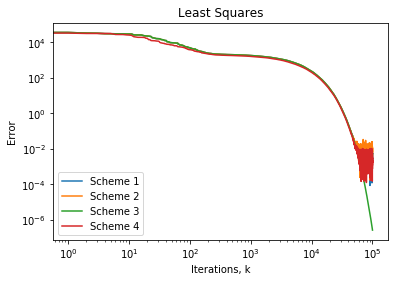
\includegraphics[scale=0.5]{tex_images/4thSchemeLS.png}
	\end{minipage}
	\quad
	\begin{minipage}[b]{0.45\linewidth}
		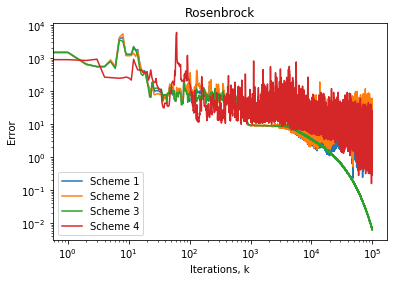
\includegraphics[scale=0.5]{tex_images/4thSchemeRosenbrock.png}
	\end{minipage}
	\end{figure}

We present a corollary to theorem \ref{August10_Theorem_ConvergenceAnalysis} when $f^* = 0$. \newline 


\textcolor{red}{Remark}: Looks like this method of drawing two independent random vectors (denoted by scheme $4$) is not any better than scheme $3$. 



\begin{corollary} \label{August18_Theorem_ConvergenceAnalysis}
Let $f^* = 0$. Assume $g_{\mu}(x) = 2F(x)^\top \left\{\frac{F(x+\mu u)-F(x)}{\mu}u\right\}$ is an unbiased estimator of $\nabla f_{\mu}(x)$. Suppose we pick 

\begin{align*}
h = \frac{1}{4\left(\frac{\mu^2}{2}L_{\nabla F}^2(n+6)^3 + (n+4)L_{\nabla f}\right)}
\end{align*}

Then the convergence rate is  

\begin{align}
\frac{1}{N+1}\sum_{k=0}^{N}(\phi_k-f^*) \leq \frac{4(n+4)L_{\nabla f}\|x_0 - x^*\|^2}{N+1} + \mu^2L_{\nabla f}n \label{August18_convergence_analysis_3}
\end{align}

where $\phi_k:= \mathbb{E}_{\mathcal{U}_{k-1}}(f(x_k))$ for $k \geq 1$ and $\phi_0:= f(x_0)$ and definition of $\mathcal{U}_{k-1}$ is in lemma \ref{July_27_lemma}. \newline 

In addition, if $f$ is $\lambda$-strongly convex and $\delta_{\mu}:= \frac{2\mu^2 nL_{\nabla f}}{\lambda}$, then the rate becomes

\begin{align}
\phi_N - f^* & \leq \frac{L_{\nabla f}}{2}\left[\delta_{\mu} + \left(1 - \frac{\lambda}{8(n+4)L_{\nabla f}}\right)^N(\|x_0 - x^*\|^2 - \delta_{\mu})\right]
\end{align}

\begin{proof}
Using $f^* = 0$ and the proof of theorem \ref{August10_Theorem_ConvergenceAnalysis}, we have 

\begin{align}
\mathbb{E}_{u_k}r_{k+1}^2 & \leq r_k^2 - \frac{f(x_k)-f^*}{4(n+4)L_{\nabla f}} + \frac{\mu^2}{4}\left[\frac{n}{n+4}\right] \label{August18_Corollary_inequality}
\end{align}

The rest follows from the proof of theorem \ref{August10_Theorem_ConvergenceAnalysis}. Next, using equation \eqref{August18_Corollary_inequality} and following the theorem \ref{August10_Theorem_ConvergenceAnalysis} analysis, we have the conclusion. 
\end{proof}

\end{corollary}

\subsection{August 19}

Recall from equation \eqref{August10_convergence_analysis_2} here:

\begin{align*}
\mathbb{E}_{u_k}r_{k+1}^2 & \leq r_k^2 - 2h[f(x_k)-f^*][1 - h\mu^2L_{\nabla F}^2(n+6)^3 - 2h(n+4)L_{\nabla f}] + \mu^2nhL_{\nabla f} + h^2[2\mu^2f^*L_{\nabla F}^2(n+6)^3] \\ & - 2h[\mathbb{E}_{u_k}g_{\mu}(x_k)-\nabla f_{\mu}(x_k)](x_k-x^*)
\end{align*}

We can proceed in proving the convergence analysis (pretty sure it works...but will finalize details later) when $f$ is strongly convex, $g_{\mu}(x_k)$ is not necesarily an unbiased estimator of $\nabla f_{\mu}(x_k)$, $F$ is not necessarily bounded, and using the fact: 

\begin{align}
|-2h[\mathbb{E}_{u_k}g_{\mu}(x_k)-\nabla f_{\mu}(x_k)](x_k-x^*) | & \leq \frac{4hL_F}{\lambda}\mu(n+3)^{3/2}L_{\nabla F}(f(x_k) - f^*) \notag \\ & + h\mu\left[\sqrt{f^*}(n+3)^{3/2}L_{\nabla F} + \frac{L_{\nabla f}}{2}(n+3)^{3/2}\right] \notag  \\ & + 2h(f(x_k) - f^*)\frac{\mu}{\lambda}\left[\sqrt{f^*}(n+3)^{3/2}L_{\nabla F} + \frac{L_{\nabla f}}{2}(n+3)^{3/2}\right] \label{August19_Result1}
\end{align}

An additional parameter we need to control in addition to Nesterov's line of reasoning is $\mu$. One remark to add: If we relax strongly convexity of $f$ to convexity, I don't see how we can use Nesterov's approach to prove convergence.  Proof to be added... \newline 

\subsection{August 20}

We continue with \eqref{August19_Result1}. First, we prove a lemma

\begin{lemma} \label{Aug20Lemma1}
Let $g_{\mu}(x) = 2F(x)^\top\left\{\frac{F(x+\mu u)-F(x)}{\mu}\right\}u$. By theorem \ref{July_13_Theorem_grad_upper_bound} and lemma $3$ in \cite{Nesterov2015}, we have 
\begin{align}
\| \mathbb{E}_ug_{\mu}(x) - \nabla f_{\mu}(x)\| \leq \mu(n+3)^{3/2}L_{\nabla F}\|F(x)\| + \frac{\mu}{2}L_{\nabla f}(n+3)^{3/2}
\end{align}

\begin{proof}
\begin{align*}
\| \mathbb{E}_ug_{\mu}(x) - \nabla f_{\mu}(x)\| & = \| 2F(x)\nabla F_{\mu}(x) - 2F(x)\nabla F(x) + \nabla f(x) - \nabla f_{\mu}(x) \| \\ & \leq \|2F(x)[\nabla F_{\mu}(x) - \nabla F(x)]\| + \| \nabla f(x) - \nabla f_{\mu}(x)\| \\ & \leq 2\|F(x)\| \|\nabla F_{\mu}(x) - \nabla F(x)\| + \|\nabla f(x) - \nabla f_{\mu}(x)\| \\ & \leq \mu(n+3)^{3/2}L_{\nabla F}\|F(x)\| + \frac{\mu}{2}L_{\nabla f}(n+3)^{3/2}
\end{align*}
\end{proof}
\end{lemma}

Using lemma \ref{Aug20Lemma1}, we prove equation \eqref{August19_Result1}. 

\begin{lemma} \label{Aug20Lemma2}
Suppose $F$ is lipschitz continuous and $f$ is $\lambda$-strongly convex. Using lemma \ref{Aug20Lemma1}, we have 

\begin{align*}
|-2h[\mathbb{E}_{u_k}g_{\mu}(x_k)-\nabla f_{\mu}(x_k)](x_k-x^*) | & \leq \frac{4hL_F}{\lambda}\mu(n+3)^{3/2}L_{\nabla F}(f(x_k) - f^*) \notag \\ & + h\mu\left[\sqrt{f^*}(n+3)^{3/2}L_{\nabla F} + \frac{L_{\nabla f}}{2}(n+3)^{3/2}\right] \notag  \\ & + 2h(f(x_k) - f^*)\frac{\mu}{\lambda}\left[\sqrt{f^*}(n+3)^{3/2}L_{\nabla F} + \frac{L_{\nabla f}}{2}(n+3)^{3/2}\right] 
\end{align*}

\begin{proof}

Since $F$ is lipschitz continuous, we have 

\begin{align*}
\|F(x) \| & \leq \|F(x) - F(x^*)\| + \|F(x^*)\| \\ & \leq L_F\|x-x^*\| + \|F(x^*)\| 
\end{align*}

By strong convexity of $f$ and Young's inequality, we have 

\begin{align*}
\|x_k-x^*\|^2 & \leq \frac{2}{\lambda}(f(x_k)-f^*) \\ \|x_k-x^*\| &  \leq \frac{1}{2} + \frac{f(x_k)-f^*}{\lambda}
\end{align*}

Continuing with the left hand side,

\begin{align*}
|-2h[\mathbb{E}_{u_k}g_{\mu}(x_k)-\nabla f_{\mu}(x_k)](x_k-x^*) | & \leq 2h \| \mathbb{E}_{u_k}g_{\mu}(x_k) - \nabla f_{\mu}(x_k)\| \|x_k-x^*\| \\ & \leq 2h[\mu(n+3)^{3/2}L_{\nabla F}\|F(x_k)\| + \frac{\mu}{2}L_{\nabla f}(n+3)^{3/2}]\|x_k-x^*\| \\ & \leq 2h[L_F\|x_k-x^*\| \mu (n+3)^{3/2}L_{\nabla F} + \|F(x^*)\|\mu (n+3)^{3/2}L_{\nabla F}]\|x_k - x^*\| \\ & +  2h[\frac{\mu}{2}L_{\nabla f}(n+3)^{3/2}]\|x_k-x^*\| \\ & = 2hL_F\|x_k-x^*\|^2\mu (n+3)^{3/2}L_{\nabla F} \\ & + 2h[\|F(x^*)\|\mu (n+3)^{3/2}L_{\nabla F} + \frac{\mu}{2}L_{\nabla f}(n+3)^{3/2}]\|x_k-x^*\| \\ & \leq \frac{4hL_F}{\lambda}(f(x_k) -f^*)\mu (n+3)^{3/2}L_{\nabla F} \\ & + 2h[\|F(x^*)\| \mu (n+3)^{3/2}L_{\nabla F} + \frac{\mu}{2}L_{\nabla f}(n+3)^{3/2}]\|x_k-x^*\| \\ & \leq \frac{4hL_F}{\lambda}(f(x_k)-f^*)\mu(n+3)^{3/2}L_{\nabla F} \\ & + h[\|F(x^*)\|\mu (n+3)^{3/2}L_{\nabla F} + \frac{\mu}{2}L_{\nabla f}(n+3)^{3/2}] \\ & + 2h\left[\frac{f(x_k)-f^*}{\lambda}\right][\|F(x^*)\|\mu (n+3)^{3/2}L_{\nabla F} + \frac{\mu}{2}L_{\nabla f}(n+3)^{3/2}]
\end{align*}
Finally, factoring $\mu$ in the second and third term and writing $\sqrt{f^*} = \|F(x^*)\|$, we have our conclusion. 
\end{proof}
\end{lemma}

Task: Using equation \eqref{August10_convergence_analysis_2},  we need to pick $h, \mu > 0$ appropriately to advance the convergence analysis. \newline 

Continuing with the convergence analysis in equation \eqref{August10_convergence_analysis_2} and using lemma \ref{Aug20Lemma2}, we have 

\begin{align}
\mathbb{E}_{u_k}r_{k+1}^2 & \leq r_k^2 - 2h[f(x_k)-f^*][\star_1] + \star_2 \label{Aug21ConvergenceAnalysis1}
\end{align}
where 
\begin{align*}
\star_1 & := 1 - h\mu^2L_{\nabla F}^2(n+6)^3 - 2h(n+4)L_{\nabla f} - \frac{2L_F}{\lambda}\mu(n+3)^{3/2}L_{\nabla F} -\frac{\mu}{\lambda}\left[\sqrt{f^*}(n+3)^{3/2}L_{\nabla F} + \frac{L_{\nabla f}}{2}(n+3)^{3/2}\right] \\ \star_2 & := h\left[\mu^2nL_{\nabla f} + \mu\left[\sqrt{f^*}(n+3)^{3/2}L_{\nabla F} + \frac{L_{\nabla f}}{2}(n+3)^{3/2}\right]\right] + h^2[2\mu^2f^*L_{\nabla F}^2(n+6)^3]
\end{align*}

Taking the expectation with respect to $\mathcal{U}_{k-1}$ (see lemma \ref{July_27_lemma}), 

\begin{align}
\rho_{k+1} & \leq \rho_k - 2h[\phi_k - f^*][\star_1] + \star_2
\end{align}

where $\rho_k$ is defined in \cite{Nesterov2015}. Applying this inequality recursively, 

\begin{align}
2h\sum_{k=0}^N(\phi_k-f^*)[\star_1] & \leq \|x_0 - x^*\|^2 + (N+1)[\star_2]
\end{align}

Rearranging yields

\begin{align}
\frac{1}{N+1}\sum_{k=0}^N(\phi_k - f^*) \leq \frac{1}{2h}\left[\frac{\|x_0 - x^*\|^2}{N+1} + [\star_2]\right]\frac{1}{[\star_1]}
\end{align}

We show a different convergence analysis result. By strong convexity of $f$, we have

\begin{align}
-(f(x_k) - f^*) & \leq -\frac{\lambda}{2}\|x_k-x^*\|^2
\end{align}

Using this and equation \eqref{Aug21ConvergenceAnalysis1}, we have 

\begin{align}
\mathbb{E}_{u_k}r_{k+1}^2 & \leq r_k^2 - \lambda hr_k^2[\star_1] + [\star_2] \notag \\ & = (1-\lambda h[\star_1])r_k^2 + [\star_2]
\end{align}

where we pick $h, \mu > 0$ appropriately so $\star_1 \in [0,1]$. \newline

Taking the expectation with respect to $\mathcal{U}_{k-1}$ yields 

\begin{align}
\rho_{k+1} & \leq (1- \lambda h [\star_1])\rho_k + \star_2
\end{align}

Using this and picking $\delta_{\mu}$ such that $\lambda h[\star_1]\delta_{\mu} = [\star_2]$ and we have 

\begin{align}
\rho_{k+1} - \delta_{\mu} & \leq (1 - \lambda h [\star_1])(\rho_k - \delta_{\mu}) \notag \\ & \leq (1 - \lambda h [\star_1])^{k+1}(\rho_0 - \delta_{\mu})
\end{align}

Since $f$ has gradient lipschitz, taking expectation and the previous equation, we have 

\begin{align}
\phi_N - f^* & \leq \frac{L_{\nabla f}}{2}\rho_N \notag  \\ & \leq \frac{L_{\nabla f}}{2}\left[\delta_{\mu} + (1 - \lambda h [\star_1])^N(\|x_0 - x^*\|^2 - \delta_{\mu})\right] \label{August24_ConvergenceRate_Bound1}
\end{align}

% \subsection{August 21}

\section{Week 11: August 24}

\subsection{August 24}

Unbiased, $f^* = 0$, see theorem \ref{August18_Theorem_ConvergenceAnalysis}: 
Convex: 

\begin{align*}
\frac{1}{N+1}\sum_{k=0}^N(\phi_k - f^*) \leq \frac{4(n+4)L_{\nabla f}\|x_0-x^*\|^2}{N+1} + \mu^2L_{\nabla f}n
\end{align*}

$f$ is $\lambda$-strongly convex: 

\begin{align*}
\phi_N - f^* & \leq \frac{L_{\nabla f}}{2}\left[\delta_{\mu} + \left(1- \frac{\lambda}{8(n+4)L_{\nabla f}}\right)^N(\|x_0 - x^*\|^2 - \delta_{\mu})\right]
\end{align*}

where $\delta_{\mu} = \frac{2\mu^2 n L_{\nabla f}}{\lambda}$. \newline 

\textcolor{red}{Nesterov's convergence rates}: \newline 

$f$ is convex: 

\begin{align*}
\frac{1}{N+1}\sum_{k=0}^{N}(\phi_k - f^*) & \leq \frac{4(n+4)L_{\nabla f}\|x_0 - x^*\|^2}{N+1} + \frac{9\mu^2 (n+4)^2 L_{\nabla f}}{25}
\end{align*}

$f$ is $\lambda$-strongly convex: 

\begin{align*}
\phi_N - f^* \leq \frac{L_{\nabla f}}{2}\left[\delta_{\mu} + \left(1 - \frac{\lambda}{8(n+4)L_{\nabla f}}\right)^N(\|x_0-x^*\|^2 - \delta_{\mu})\right]
\end{align*}
where $\delta_{\mu} = \frac{18\mu^2(n+4)^2L_{\nabla f}}{25 \lambda}$. \newline 

\textcolor{red}{Biased estimator $g_{\mu}$ of $\nabla F_{\mu}$}: \newline 

$f$ is $\lambda$-strongly convex: 

\begin{align*}
\frac{1}{N+1}\sum_{k=0}^N (\phi_k - f^*) & \leq \frac{1}{2h}\left[\frac{\|x_0 - x^*\|^2}{N+1} + \star_2\right] + \frac{1}{\star_1}
\end{align*}

\begin{align*}
\phi_N - f^* & \leq \frac{L_{\nabla f}}{2}[\delta_{\mu} + (1-\lambda h \star_1)^N(\|x_0 - x^*\|^2 - \delta_{\mu})]
\end{align*}

where $\delta_{\mu} = \frac{\star_2}{\lambda h \star_1}$ \newline 

\begin{align*}
\star_1 & := 1 - h\mu^2L_{\nabla F}^2(n+6)^3 - 2h(n+4)L_{\nabla f} - \frac{2L_F}{\lambda}\mu(n+3)^{3/2}L_{\nabla F} -\frac{\mu}{\lambda}\left[\sqrt{f^*}(n+3)^{3/2}L_{\nabla F} + \frac{L_{\nabla f}}{2}(n+3)^{3/2}\right] \\ \star_2 & := h\left[\mu^2nL_{\nabla f} + \mu\left[\sqrt{f^*}(n+3)^{3/2}L_{\nabla F} + \frac{L_{\nabla f}}{2}(n+3)^{3/2}\right]\right] + h^2[2\mu^2f^*L_{\nabla F}^2(n+6)^3] 
\end{align*}

\subsection{August 25:}

On August $5$ (see \ref{August_5_Journal_entry}), under scheme $3$, we have shown $g_{\mu}$ is an unbiased estimator of $\nabla f_{\mu}$. \newline 

Now, consider the least squares setting where $F(x) = Ax-b$. Here are the Lipschitz constants:

\begin{align*}
L_{\nabla F} & = \|A\|_2 \\ L_{\nabla F} & = 0 \\ L_{\nabla f} & = 2\|A^\top A\|_2 \\ f^* & = 0
\end{align*}

where we assumed $b \in \text{range}(A)$. We compute $\star_1, \star_2$, and $\frac{\star_2}{h\star_1}$ using these constants:

\begin{align*}
\star_1 & = 1 - 4h(n+4)\|A^\top A\|_2 - \frac{\mu}{\lambda}\left[\|A^\top A\|_2 (n+3)^{3/2}\right] \\ \star_2 & = h\left[2\mu^2 n\| A^\top A\|_2 + \mu \|A^\top A\|_2 (n+3)^{3/2} \right] \\ \frac{\star_2}{h\star_1} & = \frac{2\mu^2 n\| A^\top A\|_2 + \mu \|A^\top A\|_2 (n+3)^{3/2}}{1 - 4h(n+4)\|A^\top A\|_2 - \frac{\mu}{\lambda}\|A^\top A\|_2 (n+3)^{3/2}}
\end{align*}

\textcolor{red}{Remark}: This bound in equation \eqref{August24_ConvergenceRate_Bound1} and the previous equation yields that the error scales like $\mathcal{O}\left(\mu^2 n + \mu n^{3/2}\right)$ which is much worse than what we originally got for the unbiased estimator case where the error scales as $\mathcal{O}(\mu^2 n)$. 

\subsection{A Note from Matt}

Let's analyze things a bit differently for a new perspective on how biased estimators are screwing up our analysis. 

I'll use $g_{\mu}(x;u)$ to denote the "Scheme 3" estimator that we know and love by now. 
I'm not sure how well this jives with the notation established so far, but I've been interpreting 
$F(x):\mathbb{R}^n\to\mathbb{R}^p$ to be defined by the vector $\left[F_1(x),\dots,F_p(x)\right]$ 
and $F_{\mu}(x):\mathbb{R}^n\to\mathbb{R}^p$ to be defined by the vector $\left[F_{\mu,1}(x),\dots,F_{\mu,p}(x)\right]$,
where $F_{\mu,i}$ denotes the Gaussian (or whatever distribution) smoothed version of the function $F_{i}(x)$. 
We assume that when computing $g_{\mu}(x;u)$, a single sample $u$ from the distribution is used, i.e., a common $u$ is used
in the estimation of each entry of $F_{\mu}$. 

Let's use the classical descent lemma, and unlike Nesterov, let's look at decrease in $f$, instead of $f_{\mu}$:

$$f(x_{k+1})\leq f(x_k) - h\langle \nabla f(x_k), g_{\mu}(x_k;u)\rangle + \frac{1}{2}h^2L_{\nabla f}\|g_{\mu}(x_k;u)\|^2.$$ 

Taking expectations of both sides with respect to $u$,
$$\mathbb{E}_{u} \left[f(x_{k+1})\right] \leq f(x_k) - h\langle\nabla f(x_k), \mathbb{E}_u \left[g_{\mu}(x_k;u)\right]\rangle + \frac{1}{2}h^2 L_{\nabla f}\mathbb{E}_u\left[\|g_{\mu}(x_k;u)\|^2\right].$$%\section*{References}

Using Theorem~\ref{August_3_Theorem_1}, 
$$\mathbb{E}_{u} \left[f(x_{k+1})\right] \leq f(x_k) - h\langle\nabla f(x_k), \mathbb{E}_u \left[g_{\mu}(x_k;u)\right]\rangle + \frac{1}{2}h^2 L_{\nabla f}\left(2\mu^2f(x)L_{\nabla F}^2(n+6)^3 + 2(n+4)\|\nabla f(x)\|^2\right).$$

Now let's work on that inner product. 
We seek to \emph{lower bound} the inner product, since we intend to upper bound its negative to get anything useful. 
Reexpressing (and denoting $\nabla F_{\mu}, \nabla F$ as the Jacobians of the respective functions in $\mathbb{R}^{p\times n}$). 

$$\begin{array}{c}\vspace{1pc}
\langle\nabla f(x_k), \mathbb{E}_u \left[g_{\mu}(x_k;u)\right]\rangle = 
\langle \nabla f(x_k), 2\nabla F_{\mu}(x_k)^\top  F(x_k)\rangle =
\langle 2\nabla F(x_k)^\top F(x_k), 2\nabla F_{\mu}(x_k)^\top F(x_k)\rangle =\\
\vspace{1pc}

4F(x_k)^\top \left[\nabla F(x_k)\nabla F_{\mu}(x_k)^\top\right] F(x_k) =
4F(x_k)^\top \left[\displaystyle\sum_{i=1}^p \nabla F_{i}(x)\nabla F_{\mu,i}(x_k)^\top \right]F(x_k)
\end{array}$$

Trivially, then, since the quadratic function is a sum of outer products, 
$$\langle\nabla f(x_k), \mathbb{E}_u \left[g_{\mu}(x_k;u)\right]\rangle
\geq 4\|F(x_k)\|^2 \displaystyle\min_{i=1,\dots,p} \left[\nabla F_{\mu,i}(x_k)^\top \nabla F_i(x_k)\right]$$

So, the only way this bound is useful is if the minimum eigenvalue is bounded below by zero, i.e.,
if \emph{all} the inner products between the true gradient and the smoothed gradient are nonnegative!
I'm not totally sure how you can guarantee this algorithmically (e.g., by adaptively driving $\mu$) , but \textbf{it's an intuitive and reasonable geometric condition}. The other thing that's odd here is that we're getting a term that's effectively
$-C\|F(x)\|^2$ for $C>0$ provided the geometric condition is satisfied, when in SGD methods, one often expects to see $-C\|\nabla f(x)\|^2.$ This actually makes the analysis look more like Gauss-Newton analysis. The problem is, however, that our current bound from Theorem~\ref{August_3_Theorem_1} is giving us a SGD-type bound on the first-order Taylor remainder. 


\subsection{Closing Remarks:}

In the case $g_{\mu}(x) = 2F(x)^\top \left\{\frac{F(x+ \mu u) - F(x)}{\mu}\right\}u$ is a biased estimator of $f_{\mu}(x)$, we didn't see any theoretical improvements in the convergence rate in contrast to Nesterov's algorithms for the unstructured case; we saw a speed up on convergence empirically. My question (which may have been answered) is how common is this? \newline 

\textcolor{red}{Things I would like to have done}: I am pausing research (in general) until late December 2020 or early January 2021 to secure a full time industry position upon graduation. When research resumes, I would like to incorporate it in my PhD disseration, whatever direction we take it. If an opportunity to continue this research with Stefan exists, I would like to involve my PhD advisor in this (currently we haven't discussed about this summer project). By then, I believe I'll have enough time away from research to be recharged and make some contribution (hopefully a publication). As a reference, I am planning to graduate at the end of July 2021, so hopefully this is realistic. 

\bibliography{../bibs/smw-bigrefs,../bibs/project}
\bibliographystyle{abbrvnat} 

\end{document}

